%----------
%	Context-Aware Multi-Agent Orchestration via MCP
%	Bachelor Thesis — Universidad Carlos III de Madrid
%	Based on the official UC3M TFG LaTeX template (Biblioteca UC3M, 2019)
%----------

%----------
%	CONFIGURACIÓN DEL DOCUMENTO
%----------

\documentclass[12pt]{report}

% MÁRGENES: 2,5 cm sup. e inf.; 3 cm izdo. y dcho.
\usepackage[
a4paper,
vmargin=2.5cm,
hmargin=3cm
]{geometry}

% INTERLINEADO
\renewcommand{\baselinestretch}{1.15}
\parskip=6pt

% DEFINICIÓN DE COLORES
\usepackage[table]{xcolor}
\definecolor{azulUC3M}{RGB}{0,0,102}
\definecolor{gray97}{gray}{.97}
\definecolor{gray75}{gray}{.75}
\definecolor{gray45}{gray}{.45}

% PDF/A
\usepackage[a-1b]{pdfx}

% ENLACES
\usepackage{hyperref}
\hypersetup{colorlinks=true,
	linkcolor=black,
	urlcolor=blue}

% EXPRESIONES MATEMATICAS
\usepackage{amsmath,amssymb,amsfonts,amsthm}

\usepackage{txfonts}
\usepackage[T1]{fontenc}
\usepackage[utf8]{inputenc}

\usepackage[english]{babel}
\usepackage[babel, english=american]{csquotes}
\AtBeginEnvironment{quote}{\small}

% PIE DE PÁGINA
\usepackage{fancyhdr}
\pagestyle{fancy}
\fancyhf{}
\renewcommand{\headrulewidth}{0pt}
\rfoot{\thepage}
\fancypagestyle{plain}{\pagestyle{fancy}}

% TÍTULOS
\usepackage{titlesec}
\usepackage{titletoc}
\titleformat{\chapter}[block]
{\large\bfseries\filcenter}
{\thechapter.}
{5pt}
{\MakeUppercase}
{}
\titlespacing{\chapter}{0pt}{0pt}{*3}
\titlecontents{chapter}
[0pt]
{}
{\contentsmargin{0pt}\thecontentslabel.\enspace\uppercase}
{\contentsmargin{0pt}\uppercase}
{\titlerule*[.7pc]{.}\contentspage}

\titleformat{\section}
{\bfseries}
{\thesection.}
{5pt}
{}
\titlecontents{section}
[5pt]
{}
{\contentsmargin{0pt}\thecontentslabel.\enspace}
{\contentsmargin{0pt}}
{\titlerule*[.7pc]{.}\contentspage}

\titleformat{\subsection}
{\normalsize\bfseries}
{\thesubsection.}
{5pt}
{}
\titlecontents{subsection}
[10pt]
{}
{\contentsmargin{0pt}
	\thecontentslabel.\enspace}
{\contentsmargin{0pt}}
{\titlerule*[.7pc]{.}\contentspage}

% TABLAS (estilo ingeniería)
\usepackage{multirow}
\usepackage{caption}
\usepackage{floatrow}
\usepackage{array}
\newcolumntype{P}[1]{>{\centering\arraybackslash}p{#1}}
\DeclareCaptionFormat{upper}{#1#2\uppercase{#3}\par}
\usepackage{booktabs}
\usepackage[htt]{hyphenat}
\usepackage{makecell}

\captionsetup[table]{
	format=upper,
	justification=centering,
	labelsep=period,
	width=.75\linewidth,
	labelfont=small,
	font=small,
}

% FIGURAS (estilo ingeniería)
\usepackage{graphicx}
\graphicspath{{imagenes/}{figures/}}

\captionsetup[figure]{
	format=hang,
	name=Fig.,
	singlelinecheck=off,
	labelsep=period,
	labelfont=small,
	font=small
}

% NOTAS AL PIE
\usepackage{chngcntr}
\counterwithout{footnote}{chapter}

% LISTADOS DE CÓDIGO
\usepackage{listings}

\lstdefinestyle{estilo}{ frame=Ltb,
	framerule=0pt,
	aboveskip=0.5cm,
	framextopmargin=3pt,
	framexbottommargin=3pt,
	framexleftmargin=0.4cm,
	framesep=0pt,
	rulesep=.4pt,
	backgroundcolor=\color{gray97},
	rulesepcolor=\color{black},
	%
	basicstyle=\ttfamily\footnotesize,
	keywordstyle=\bfseries,
	stringstyle=\ttfamily,
	showstringspaces = false,
	commentstyle=\color{gray45},
	%
	numbers=left,
	numbersep=15pt,
	numberstyle=\tiny,
	numberfirstline = false,
	breaklines=true,
	xleftmargin=\parindent
}

% Style for shell/CLI sessions: no line numbers, keeps output readable
\lstdefinestyle{cli}{
	frame=Ltb,
	framerule=0pt,
	aboveskip=0.5cm,
	framextopmargin=3pt,
	framexbottommargin=3pt,
	framexleftmargin=0.4cm,
	framesep=0pt,
	rulesep=.4pt,
	backgroundcolor=\color{gray97},
	rulesepcolor=\color{black},
	basicstyle=\ttfamily\footnotesize,
	numbers=none,
	breaklines=true,
	xleftmargin=0.4cm
}

% JSON language
\lstdefinelanguage{json}{
	morestring=[b]",
	morecomment=[l]{//},
	sensitive=true
}

\captionsetup[lstlisting]{font=small, labelsep=period}
\lstset{style=estilo}
\renewcommand{\lstlistingname}{\uppercase{Code}}

% DIAGRAMAS
\usepackage{tikz}
\usetikzlibrary{shapes.geometric, arrows.meta, positioning, fit, calc}
\usepackage{pgfplots}
\pgfplotsset{compat=1.18}

% TODO markers and result placeholders
\newcommand{\fillme}[1]{\textcolor{red}{\textbf{[TODO: #1]}}}
\newcommand{\resultslot}[2][5.5cm]{%
	\begin{center}
	\fbox{\parbox[c][#1][c]{0.88\linewidth}{\centering\small\itshape --- Results slot pending ---\\[2pt]#2}}
	\end{center}}

% BIBLIOGRAFÍA (IEEE)
\usepackage[backend=biber, style=ieee, isbn=false,sortcites, maxbibnames=5, minbibnames=1]{biblatex}
\addbibresource{bibliografia/bibliografia.bib}

% APÉNDICES
\usepackage{appendix}

%-------------
%	DOCUMENTO
%-------------

\begin{document}
\pagenumbering{roman}

%----------
%	PORTADA
%----------
\begin{titlepage}
	\begin{sffamily}
	\color{azulUC3M}
	\begin{center}
		\begin{figure}[H]
			\makebox[\textwidth][c]{
\includegraphics[width=16cm]{Portada_Logo.png}}
		\end{figure}
		\vspace{2.5cm}
		\begin{Large}
			Bachelor's Degree in Data Science and Engineering\\
			Academic Year 2025--2026\\
			\vspace{2cm}
			\textsl{Bachelor Thesis}
			\bigskip

		\end{Large}
		 	{\Huge ``Context-Aware Multi-Agent Orchestration: A Standardized Architecture via MCP for Autonomous Agentic Systems''}\\
		 	\vspace*{0.5cm}
	 		\rule{10.5cm}{0.1mm}\\
			\vspace*{0.9cm}
			{\LARGE Arturo Javier Kolster Borges}\\
			\vspace*{1cm}
		\begin{Large}
			Boni García Gutiérrez\\
			Legan\'es, September 2026\\
		\end{Large}
	\end{center}
	\vfill
	\color{black}
	
\includegraphics[width=4.2cm]{imagenes/creativecommons.png}\\
	This work is licensed under Creative Commons \textbf{Attribution -- Non Commercial -- Non Derivatives}
	\end{sffamily}
\end{titlepage}

\newpage
\thispagestyle{empty}
\mbox{}

%----------
%	RESUMEN
%----------
\renewcommand\abstractname{\large\uppercase{Summary}}
\begin{abstract}
\thispagestyle{plain}
\setcounter{page}{3}


This thesis presents \emph{thelab-mcp}, a local-first, multi-agent orchestration architecture built on the Model Context Protocol (MCP), a standardized communication protocol between LLM-based agents and local or external data environments. The architecture presented is an autonomous machine learning (ML) factory that converts a local tabular dataset into a versioned, validated, locally served ML model, with a single human approval gate and no mandatory cloud dependency.

The system is designed around the separation of responsibilities. Large language models decide \emph{what} to run, while a deterministic Python pipeline executes \emph{how} it runs. Typed contracts (Pydantic), a SQLite+FTS5 context store, seven MCP servers, an AST-restricted code sandbox, and a single human approval gate connect the agentic layer to the deterministic core. Agents (an analyst, a feature engineer, and a model selector, coordinated through an orchestrator) can only propose and compute inside bounded, sandboxed rounds. Every execution is recorded as evidence in run manifests, every claim an agent makes must resolve to recorded metrics, and a rejected proposal can never be executed. The design principle is \emph{grounded autonomy}. The deterministic factory provides the grounding evidence, and the agents operate on top of it as an additional layer.

The evaluation answers six research questions in two groups. The \emph{system group} is verified by an automated evaluator that runs inside a disposable temporary workspace. (RQ1) A model-training run is reproducible from its dataset, configuration, and seed. (RQ2) An independent MCP client can discover and use a registered model without any knowledge of the training internals. (RQ3) Local context retrieval recovers past evidence without modifying the store. The \emph{agentic group} measures what the agent layer adds on top of that grounding. (RQ4) Context-grounded agents produce more verifiable proposals than ungrounded agents. (RQ5) Sandboxed agent-generated code trains valid, competitive models beyond the fixed deterministic grid. (RQ6) Role-specialized agents coordinated via MCP outperform a single shared-prompt agent.

Different experiments complemented the automated checks. A three-ways-in comparison (CLI, HTTP, MCP) showed identical results across the interfaces. A real-dataset validation demonstrated correct and traceable exploratory data analysis and cleaning policies. Grounded and ungrounded agentic rounds showed that context produces actual verifiable claims instead of guesses. Sandboxed agent code managed to train valid and competitive models beyond the fixed grid. Role-specialized coordination outperformed single shared prompts. Multi-domain stress validation across ten datasets, from genomics and health to crypto, energy, and finance, surpassed the baseline models and generated an absorption loop to improve the deterministic pipeline. A fully-offline execution with a local 3B model demonstrated the architecture's independence from any cloud provider.

The results support the hypothesis. The architecture executes reproducible data-to-model workflows and exposes their artifacts to independent agents without being limited to any specific LLM provider. Its limitations (sandbox filesystem confinement, stdio-only transport, dataset-specific agentic findings) are documented as concrete, traceable findings rather than omitted.

\textbf{Keywords:} Multi-agent systems, Model Context Protocol, reproducibility, machine learning pipelines, interoperability, context engineering, local-first software.


	\vfill
\end{abstract}
	\newpage
	\thispagestyle{empty}
	\mbox{}

%----------
%	DEDICATORIA
%----------
\chapter*{Dedication}

\setcounter{page}{5}

	To my family, especially to my parents, for their unconditional support through these years. To my friends, and to everyone I have met during the bachelor's degree, for making the journey worth it far beyond the classroom. To Universidad Carlos III de Madrid, for being an amazing institution and a great place to learn. And to the open source community, whose tools and generosity have made this work possible.


	\vfill

	\newpage
	\thispagestyle{empty}
	\mbox{}

%----------
%	ÍNDICES
%----------
\tableofcontents
\thispagestyle{fancy}

\newpage
\thispagestyle{empty}
\mbox{}

\listoffigures
\thispagestyle{fancy}

\newpage
\thispagestyle{empty}
\mbox{}

\listoftables
\thispagestyle{fancy}

\newpage
\thispagestyle{empty}
\mbox{}

%----------
%	ABBREVIATIONS
%----------
\chapter*{List of Abbreviations}
\addcontentsline{toc}{chapter}{List of Abbreviations}
\thispagestyle{fancy}

\begin{table}[H]
\begin{tabular}{p{2.8cm}p{11.5cm}}
\textbf{AC} & Acceptance Criterion \\
\textbf{AI} & Artificial Intelligence \\
\textbf{ANSI} & American National Standards Institute \\
\textbf{API} & Application Programming Interface \\
\textbf{AST} & Abstract Syntax Tree \\
\textbf{CC} & Creative Commons (license family) \\
\textbf{CLI} & Command-Line Interface \\
\textbf{CSV} & Comma-Separated Values \\
\textbf{DTO} & Data Transfer Object \\
\textbf{EDA} & Exploratory Data Analysis \\
\textbf{FTS5} & Full-Text Search engine, version 5 (SQLite module) \\
\textbf{GDPR} & General Data Protection Regulation (EU) 2016/679 \\
\textbf{HTTP} & HyperText Transfer Protocol \\
\textbf{IDE} & Integrated Development Environment \\
\textbf{JSON} & JavaScript Object Notation \\
\textbf{JSONL} & Line-delimited JSON \\
\textbf{LLM} & Large Language Model \\
\textbf{LOC} & Lines Of Code \\
\textbf{MCP} & Model Context Protocol \\
\textbf{ML} & Machine Learning \\
\textbf{MLOps} & Machine Learning Operations \\
\textbf{PII} & Personally Identifiable Information \\
\textbf{PoC} & Proof of Concept \\
\textbf{PRD} & Product Requirements Document \\
\textbf{RAG} & Retrieval-Augmented Generation \\
\textbf{RLIMIT} & Resource limit (POSIX \texttt{setrlimit}) \\
\textbf{RQ} & Research Question \\
\textbf{S\&P} & Standard \& Poor's (financial data provider) \\
\textbf{SSE} & Server-Sent Events \\
\textbf{STDIO} & Standard Input/Output (transport) \\
\textbf{SVM} & Support Vector Machine \\
\textbf{TS} & TypeScript \\
\textbf{UC3M} & Universidad Carlos III de Madrid \\
\textbf{UI} & User Interface \\
\textbf{XSS} & Cross-Site Scripting \\
\end{tabular}
\end{table}


%----------
%	TRABAJO
%----------
\clearpage
\pagenumbering{arabic}

\chapter{Introduction}
\label{ch:introduction}

\section{Motivation}
\label{sec:motivation}

Machine learning (ML) work has traditionally been organized around notebooks, scripts, and interactive experimentation. The arrival of large language models (LLMs) capable of using tools and reasoning over several steps opened a new possibility in this landscape: software in which LLM-based agents read data, propose experiments, run code, and interpret results with some degree of autonomy. The most common commercial platforms for this new wave of \emph{agentic} ML share three traits: they are mostly cloud-first, they keep context, prompts and data on external infrastructures, and reproducibility is a best-effort property rather than a guarantee. Familiar examples are OpenAI's ChatGPT data-analysis mode, Anthropic's Claude Code, and the agent tooling of cloud ML suites such as Google Vertex AI and Databricks.

The Lab defends three design positions: produce local context that both humans and agents can use; execute through a deterministic pipeline instead of letting agents decide all the steps; and use the Model Context Protocol (MCP) as the standard way to share that context, so the base stays open to any provider. Cloud and local models are supported, making the architecture model agnostic.

The concrete result is \href{https://github.com/ArturoJKB/the-lab-mcp-tfg/tree/main}{\emph{thelab-mcp}}: a multi-agent orchestration system built with the MCP protocol that ingests and converts data into versioned, validated and locally served ML models, recording every intermediate step as inspectable evidence. We can summarize the product with a metaphor that also names it: the infrastructure is \emph{the lab}, and the models, agents, and applications it produces are \emph{the experiments} run inside it.

One design rule was present through the whole development of the project, from the first prototypes to the current version: \emph{LLMs decide what to run; deterministic code executes it}. The idea behind it was to create an agentic layer on top of a deterministic pipeline. In this case, for machine learning model generation, it provides LLM agents a set of predefined deterministic tools to choose from. These range from data ingestion, exploration and cleaning to model training, evaluation, validation and hosting.

Agents can propose experiments, interpret results, write sandboxed code, and answer questions. Training and metric computation are reserved for the deterministic Python pipeline, and everything an agent starts sits behind one human approval gate. This rule is what makes reproducibility and auditability possible.

\section{Problem statement}
\label{sec:problem}

The problem addressed by this thesis can be stated as follows: \emph{design, implement, and evaluate an orchestration architecture that allows LLM-based agents to participate in a data-to-model ML workflow while keeping the workflow reproducible and auditable}.

Three sub-problems can be decomposed from the statement:

\begin{itemize}
	\item \textbf{Reproducibility.} A model-training run must be exactly reproducible from its dataset, configuration, and random seed. The context needed to reproduce the run is then stored in machine-readable form.
	\item \textbf{Interoperability.} An independent agent (one that does not share code with the system) must be able to discover and use the produced models through a standard protocol, without being granted access to the training pipeline internals.
	\item \textbf{Useful context.} The system must record what has happened during sessions (runs, decisions, errors, agent sessions) without leaking any secrets and without corrupting records.
\end{itemize}

Agentic behavior is non-deterministic by nature. The answer this thesis explores is not to make agents deterministic, but to bound them. Agents work on typed contracts. Agent-initiated execution needs human approval. Generated code runs only inside a restricted sandbox, and its output is validated deterministically before it can reach training. And every claim an agent makes is checked against recorded evidence.

\section{Objectives}
\label{sec:objectives}

The four registered objectives are the following:

\begin{itemize}
	\item (1) a \emph{state-of-the-art analysis} of context engineering and standardized communication protocols for AI agents;
	\item (2) an \emph{architectural framework}: a scalable, MCP-based architecture that splits agent logic from data sources;
	\item (3) \emph{experimental validation} through a proof of concept in a real-world technical scenario;
	\item (4) a \emph{performance evaluation} analyzing the impact of the orchestration on context optimization, token efficiency, success rates and costs.
\end{itemize}

The general objective of this thesis is to fulfill these objectives through an autonomous ML factory, autonomous in its data-to-model execution and human-gated at every agentic boundary, used as the architecture's demonstrator.

More specific objectives can be derived from the ones above:

\begin{enumerate}
	\item \textbf{O1, Deterministic factory (reg.\ objective 2, 3).} Implementation of a deterministic, local data-to-model pipeline (validation, profiling, contract generation, training, re-validation, registration) that produces a complete, self-describing artifact set per run.
	\item \textbf{O2, Typed contracts (reg.\ objective 2).} Defined typed contracts (\texttt{TaskSpec}, \texttt{RunManifest}, \texttt{ArtifactRef}, \texttt{DatasetSpec}, \texttt{ModelSpec}, \texttt{LogEntry}) that every component, human or agent, has to use to exchange information (decoupling agent logic from data sources).
	\item \textbf{O3, MCP surface (reg.\ objective 2).} Expose the factory through Model Context Protocol servers so independent agents can discover and interact with datasets, models, artifacts, and context without importing pipeline code.
	\item \textbf{O4, Context store (reg.\ objective 2, 4).} Implementation of a local, redacted, searchable evidence store (SQLite + FTS5) with read-only retrieval. Every entry is stored with a fingerprint, so the same event is never duplicated or overwritten. This store is the context-management layer of the architecture.
	\item \textbf{O5, Agentic layer with human oversight (reg.\ objective 2, 3).} Implementation of a provider-agnostic agent layer (role-specialized analyst, feature-engineer, and model-selector agents coordinated by an orchestrator, plus a grounded chat agent) that proposes experiments, computes in a sandbox, and records its activity.
	\item \textbf{O6, Evaluation (reg.\ objective 1, 3, 4).} Execute the state-of-the-art analysis (Chapter~\ref{ch:background}); formulate the six research questions; verify them with an automated evaluator; complement them with experiments on real and public datasets at increasing scale; and characterize agent reliability with task success rates and token-efficiency measurements (Section~\ref{sec:agentmetrics}).
\end{enumerate}

\section{Hypothesis and research questions}
\label{sec:hypothesis}

The working hypothesis of this thesis is:

\begin{quote}
	A local multi-agent orchestration architecture based on typed contracts and MCP capabilities that can execute reproducible data-to-model workflows and expose the resulting artifacts to independent agents without being coupled to a specific LLM provider.
\end{quote}

The hypothesis can be operationalized as six research questions in two groups. The \textbf{system group} verifies the properties any agentic layer depends on:

\begin{description}
	\item[RQ1 (Reproducible run).] Can a model-training run be reproduced using the same dataset version, configuration, dependency versions, and random seed?
	\item[RQ2 (MCP interoperability).] Can an independent MCP client discover and use a registered model without knowing the internal training-pipeline implementation?
	\item[RQ3 (Context retrieval).] Can local structured context retrieval recover useful information about previous runs, decisions, errors, snippets, and artifacts?
\end{description}

The \textbf{agentic group} measures the value the agent layer adds on top of that grounding:

\begin{description}
	\item[RQ4 (Grounding).] Do agents grounded in the local context store produce more verifiable proposals than ungrounded agents?
	\item[RQ5 (Agentic capability).] Can sandboxed agent-generated code train valid, competitive models beyond the fixed deterministic grid?
	\item[RQ6 (Orchestration value).] Do role-specialized agents coordinated via MCP outperform a single shared-prompt agent?
\end{description}


\section{Scope}
\label{sec:scope}

The system works on \emph{tabular} machine learning on a single machine: classification and regression over CSV datasets, with nine scikit-learn model families, ingestion of Kaggle datasets with automatic context packs, a local context store, and a web workspace. On top of that deterministic core sits the agentic layer (Chapter~\ref{ch:design}): agents explore data inside a code sandbox while training, metric computation and validation remain deterministic.

Deep learning and GPU training, trading and order execution, multi-user deployments, public cloud hosting, and language-model fine-tuning are out of scope for this project. However, one boundary stays open on purpose: the sandbox limits the time, memory, and libraries of the generated code, but it does not isolate that code from the files of the machine. Real file isolation needs operating-system support, and it is documented as future work. The decision and its risks are documented in the limitations (Section~\ref{sec:limitations}).


\section{Contributions}
\label{sec:contributions}

The contributions of this thesis are:

\begin{enumerate}
	\item \textbf{An architecture} for auditable agentic ML. LLMs make the decisions and a deterministic pipeline executes them, connected through typed contracts and a single human approval gate. On top of it, a grounded autonomy round lets role-specialized agents explore beyond the deterministic grid. The agents start from the pipeline's artifacts, and their output is validated deterministically.
	\item \textbf{A working implementation} of approximately 16{,}900 lines of Python plus a React/TypeScript workspace. It includes the deterministic factory, seven MCP servers, a redacted context store, a provider-agnostic agent layer with per-role prompt contracts, and an AST-restricted code sandbox. It is verified by 546 automated tests.
	\item \textbf{An automated evaluation protocol} (\texttt{evaluate\_thesis.py}). Every check runs inside a disposable temporary workspace. RQ1--RQ3 run on every demand, and the agentic questions (RQ4--RQ6) use comparison runs that measure what grounding, generated code, and role specialization each add. Four recorded experiments complement it on fixture, real and public (Kaggle) data, comparing different LLM providers.
	\item \textbf{An honest record of limitations}. It includes an adversarial audit of the full system, more than 500 checks across the CLI, HTTP service, MCP surface, and sandbox, plus an internal review of the project's agentic performance, which found five defects (an SSE serialization crash, hyperparameter-grid misapplication, a fixtures-cleaning restriction, a phantom approval principal, and a feature-name mismatch), all fixed and regression-tested. The findings, both fixed and open, are documented as evidence.
\end{enumerate}


\section{Document structure}
\label{sec:structure}

The rest of this document follows the IMRAD convention.

\textbf{Chapter~\ref{ch:background}} reviews the technical background (LLM agents, MCP, context engineering, MLOps) and related work (multi-agent frameworks, agent benchmarks, experiment-tracking platforms), closing with the gap this thesis addresses. \textbf{Chapter~\ref{ch:design}} presents the design of {\emph{thelab-mcp}}: principles, architecture, contracts, deterministic pipeline, context store, MCP surface, agent layer with its approval gate and agentic round, and safety model. \textbf{Chapter~\ref{ch:implementation}} describes the implementation: the three usage surfaces, reproducibility engineering, and the development process itself. \textbf{Chapter~\ref{ch:methodology}} defines the evaluation methodology: the six research questions, pass criteria, the automated evaluator, and the four experiments. \textbf{Chapter~\ref{ch:results}} reports the results, deterministic (RQ1--RQ3) and agentic (RQ4--RQ6). \textbf{Chapter~\ref{ch:discussion}} discusses the findings, the limitations and threats, the regulatory framework (Section~\ref{sec:regulatory}), and the socio-economic environment (Section~\ref{sec:socioeconomic}). \textbf{Chapter~\ref{ch:conclusions}} concludes and outlines future work. The annexes also contain a reproduction guide and a real run manifest.

\chapter{Background and State of the Art}
\label{ch:background}

This chapter reviews the concepts on which \emph{thelab-mcp} is built and the prior work it relates to. Sections~\ref{sec:bg-llm}--\ref{sec:bg-mcp} cover large language models, tool-using agents, and the Model Context Protocol. Section~\ref{sec:bg-context} discusses context engineering and why a local, verifiable context store is used. Section~\ref{sec:bg-mlops} reviews reproducibility and experiment tracking in MLOps. Section~\ref{sec:bg-frameworks} compares multi-agent frameworks, and Section~\ref{sec:bg-gap} states the gap this thesis addresses.

\section{Large language models and agents}
\label{sec:bg-llm}

\subsection{From transformers to instruction-following assistants}

The story of modern large language models begins in 2017, when the Transformer architecture \cite{vaswani2017attention} replaced the older recurrent designs with a mechanism based on attention. It turned out to work and scale surprisingly well, setting the base architecture for future work in the artificial intelligence field. The next chapter was size: GPT-3 \cite{brown2020gpt3} showed that training even larger Transformers on more text produced few-shot learning, meaning the model could attempt tasks it was never explicitly trained for. But a big model that only completes text is not an assistant, so the following step was behaviour: instruction tuning \cite{ouyang2022instructgpt} aligned raw models to follow user instructions, producing the assistant-style systems that agentic applications are built on. The last piece was reasoning. Chain-of-thought prompting \cite{wei2022cot} showed that asking the model to write out intermediate steps highly improved multi-step tasks, and multi-step reasoning is exactly what an agent does when it plans an experiment.

\subsection{Tool use and the agent loop}

Talking was only the first capability, and on its own it was not very useful: a model that writes perfect instructions cannot read your data or run your code. The fix was giving the models access to tools. ReAct \cite{yao2023react} showed in 2022 that the strongest pattern interleaved reasoning with action: the model thinks, calls a tool, reads the result, and thinks again. Toolformer \cite{schick2023toolformer} went one step earlier in the pipeline and showed that models could even learn \emph{when} a tool call is needed, from self-supervised data. From these results the standard agent design was created. So from it, we can define an agent as a system composed of an LLM, a harness that mediates its execution, and the set of tools it may call \cite{sutton2019bitter}. The model receives a conversation history and a list of tool specifications, it either writes text or emits structured tool calls, the harness executes them and appends the results, and the cycle repeats until a final answer or a step budget is reached. Reflexion \cite{shinn2023reflexion} closed the loop by showing that failures fed back to the models as context improved the next attempts. For this thesis the takeaway of the whole line of work is simple: what an agent \emph{knows} is decided by what its harness supplies, the set of tools and the specific context.

\subsection{Multi-agent systems}

Once single agents worked, the natural next idea was to give them roles. MetaGPT \cite{hong2023metagpt} assigned software-company positions to agents and reported more coherent output, and generative-agent simulations \cite{park2023generative} showed that memory and reflection produce believable behaviour with fewer errors. With role specialization each agent narrows its prompt, tools, and grounding to one responsibility. The problem with more agents working together is the coordination complexity it adds to the equation as well as a larger surface through which errors can spread out. \emph{thelab-mcp} takes a middle position: each agent has a role, a distinct prompt and an allowed tool list, generated code runs only in the sandbox and is validated deterministically, and training itself always stays in the deterministic factory (Section~\ref{sec:bg-frameworks} compares this with heavier frameworks).

\section{The Model Context Protocol}
\label{sec:bg-mcp}

By 2024 agents were multiplying, and so was a practical problem: every integration between an application and a model was custom work. In November 2024 Anthropic published the Model Context Protocol (MCP) \cite{mcp2024spec,mcp2024announce}, an open protocol that standardized the way applications communicate with LLMs and provide context and tools. It follows a client--server model: a host application (an agent, an IDE extension, a CLI) embeds an MCP client that connects to one or more MCP \emph{servers}, each exposing three primitives: \emph{tools} (model-invoked functions with JSON schemas), \emph{resources} (application-driven data), and \emph{prompts} (user-selected templates). Messages are JSON-RPC 2.0, and the reference transports are \texttt{stdio} (local servers spawned as subprocesses) and HTTP with server-sent events (remote servers).

MCP matters for this thesis for three reasons. The first is interoperability, which is actually the base of the protocol: "Any client that speaks MCP can use an MCP server", without sharing code with it and without knowing how it works inside. A model registry exposed over MCP can therefore be consumed by an agent that knows nothing else about the system. The second is typed tools. Every tool declares an input schema, so the requests of the model become validated as structured calls. In \emph{thelab-mcp} the schemas also set the boundaries and reject unknown fields, via the typed-contract philosophy of Chapter~\ref{ch:design}. The third is local deployment. The \texttt{stdio} transport runs each server as a small program on the user's machine, so the shared context stays local.


\section{Context engineering and local memory}
\label{sec:bg-context}

Once agents started doing more and more real work, people realized that one of the main issues was deciding what information goes into the model's context window. This practice
was named context engineering \cite{horthy2025twelvefactor,bonigarcia2025context}, and its central question is memory: what happened before, and how can an agent recover it?

The mainstream answer is retrieval-augmented generation (RAG): embed documents into a vector database, retrieve by semantic similarity, and inject the results into the prompt. RAG is a powerful solution that works really well with LLM-based agents, but for this project it brought costs that did not fit the scope. As it usually adds a cloud or heavyweight local dependency, its retrieval quality is hard to verify, and its results are not easy for a human to audit by inspecting the store.

So the decision was to use a simpler solution: a local, structured, full-text context store. Evidence (run manifests, decisions, errors, agent session summaries) is written to SQLite with an FTS5 full-text index \cite{sqlite2024fts5}, redacted at write time, fingerprinted with SHA-256 so the same event is never duplicated or overwritten, and retrieved read-only. Search is keyword-based with structured filters (run id, tags, event type, time range). Every stored entry is inspectable, every search is reproducible, and the store's bytes are unchanged by reads, a property that RQ3 asserts. Semantic hybrid search is part of future work (Section~\ref{sec:futurework}).

\section{MLOps, reproducibility, and provenance}
\label{sec:bg-mlops}

In Machine Learning reproducibility is a foundational requirement of experimental work, and is a well-documented field. For example, the JMLR reproducibility program \cite{pineau2021jmlr} turned the problems that appear in practice into concrete checks for published papers. The industry answer was experiment tracking: platforms such as MLflow \cite{zaharia2018mlflow} and DVC \cite{dvc2024} persist parameters, metrics, and artifacts per run.

These three practices were part of the inspiration of the project. The run is the unit of record: every training execution produces a run directory with a manifest (inputs hash, configuration, seed, dependency versions, statuses), metrics, and artifact references, the same mental model as MLflow's runs but implemented with local files and JSON instead of a server. The seed is the mandatory, recorded argument of every run. It is injected into every estimator, and the evaluator verifies that two identical seeded runs reproduce identical metrics. Finally, validation works as a gate: a model is only registered and servable after its run is validated and approved.

Additionally, real-world tabular data adds one more problem: \emph{leakage}, features that encode information not available at prediction time, which inflate metrics and degrade production performance \cite{kaufman2012leakage}. The cleaning policy of Chapter~\ref{ch:design} and the leakage study in Chapter~\ref{ch:results} deal with this problem concretely.

\section{Multi-agent and agent frameworks}
\label{sec:bg-frameworks}

The frameworks in Table~\ref{tab:frameworks} arrived from the orchestration side of the story, and they solve real problems: AutoGen \cite{wu2023autogen} made LLM-to-LLM conversation programmable, LangGraph \cite{langgraph2024} turned agent flows into stateful graphs, CrewAI \cite{crewai2024} packaged role-based crews, PydanticAI \cite{pydanticai2024} added typed tool layers, and Semantic Kernel \cite{semantickernel2024} connected the Microsoft plugin ecosystem.

\begin{table}[H]
\centering
\caption{Multi-agent frameworks compared with \emph{thelab-mcp}'s approach.}
\label{tab:frameworks}
\small
\begin{tabular}{p{2.6cm}p{3.3cm}p{2.6cm}p{2.6cm}p{2.6cm}}
\toprule
\textbf{System} & \textbf{Model} & \textbf{Local-first} & \textbf{Provider} & \textbf{Auditability} \\
\midrule
AutoGen \cite{wu2023autogen} & Conversable agents; LLM-to-LLM chat & Partial (cloud LLMs typical) & OpenAI-style & Conversation logs \\
LangGraph \cite{langgraph2024} & Stateful graphs of agent nodes & Partial & Agnostic via LangChain & Graph state/checkpoints \\
CrewAI \cite{crewai2024} & Role-based crews & Partial & Agnostic & Task outputs \\
PydanticAI \cite{pydanticai2024} & Typed agent + tool layer & Partial & Agnostic & Typed results \\
Semantic Kernel \cite{semantickernel2024} & Planners + plugins & Partial & Microsoft-centric & Plugin traces \\
\midrule
\textbf{\emph{thelab-mcp}} & Contracts + deterministic factory; bounded agent round & Context and evidence local & Agnostic (4 adapters) & Manifests + redacted store \\
\bottomrule
\end{tabular}
\end{table}

Most frameworks orchestrate \emph{LLM calls} and assume cloud LLM access as the default deployment. However, \emph{thelab-mcp} orchestrates \emph{work}, of which LLM calls are one part of it, alongside the deterministic pipeline, context store, and MCP servers. It also allows local LLM wiring and even works without any LLM provider. The deterministic pipeline can run without agents: agents are a layer on top of the pipeline, not the whole pipeline.


\subsection{Benchmarks for ML and data-science agents}
\label{sec:bg-benchmarks}

Another line of work tests agents as \emph{machine-learning practitioners}. MLE-bench puts them on Kaggle-style ML engineering tasks \cite{chan2024mlebench}, DS-1000
tests data-science code generation \cite{lai2023ds1000}, DSBench and TML-Bench measure end-to-end data-science and tabular-ML work \cite{jing2024dsbench,zhao2026tmlbench}, and AstaBench covers the scientific workflow \cite{matthews2025astabench}. With this project the aim was slightly different. The question was not so much whether the agent can win the task, but whether it can win and the system can prove what happened. Do runs reproduce, can an independent client consume the results, and does the evidence survive retrieval intact? The two approaches complement each other, and a capability benchmark is the natural next evaluation move (Section~\ref{sec:futurework}). Additionally, the Kaggle-style task formats directly inspired the Experiment 4 design.

\section{Gap analysis}
\label{sec:bg-gap}

The reviewed landscape exhibits a clear gap. Experiment trackers (MLflow, DVC) provide provenance but no agentic participation. Agent frameworks provide orchestration but treat the ML workflow as conversation, with weak provenance and cloud-first defaults. Commercial agentic-ML products combine both but restrict the user to external infrastructure and opaque execution. What is missing, and what this thesis tries to contribute, is a system that is simultaneously:

\begin{itemize}
	\item \textbf{complete} end-to-end (dataset $\rightarrow$ validated model $\rightarrow$ served inference), not a component library;
	\item \textbf{evidence-local} (datasets, run evidence, and context stay on the user's machine; every LLM provider is optional and swappable);
	\item \textbf{auditable by construction} (typed contracts, manifests, redaction, approval records, rejection-as-evidence); and
	\item \textbf{interoperable} through a standard protocol (MCP), so independent agents can consume the factory safely.
\end{itemize}

\emph{thelab-mcp} is designed to occupy exactly this intersection, and its behavior has been empirically validated during development across recorded runs on real data --- including failed rounds and honest refusals.

\chapter{System Design: \emph{thelab-mcp}}
\label{ch:design}

This chapter presents the design of \emph{thelab-mcp}. Section~\ref{sec:principles} states the design principles; Section~\ref{sec:arch} gives the architecture overview; Sections~\ref{sec:contracts}--\ref{sec:mcp} describe the typed contracts, the deterministic pipeline, the context store, and the MCP surface; Section~\ref{sec:agents} details the agent layer; Section~\ref{sec:lifecycle} covers the experiment lifecycle; Section~\ref{sec:ui} describes the workspace UI; and Section~\ref{sec:safety} consolidates the safety model.

\section{Design principles}
\label{sec:principles}

Five principles were established at the start of the project before any code was written and have been preserved throughout the development:

\begin{enumerate}
	\item \textbf{Deterministic core first.} ``The first usable milestone must work without a UI, an LLM, or network access.'' The factory must be complete and useful before any intelligence is layered on; agents amplify the factory but do not substitute it.
	\item \textbf{LLMs decide; deterministic code executes.} Language models propose experiments, interpret results, and answer questions. The training pipeline, cleaning, and inference are preserved to run through the same deterministic Python path. This is the invariant that makes RQ1 possible at all: an LLM that trains models itself would inject non-determinism into the very thing being measured.
	\item \textbf{Agents autonomy.} Agent-initiated execution requires explicit human approval through a single gate and generated code always passes the sandbox and a deterministic validator. Nothing an agent writes is ever executed directly, and a rejected proposal can never be executed at all.
	\item \textbf{Rejection as a first-class outcome.} A run that fails validation is a valid, traceable result (complete with manifest, validation report, and reason) not an error to swallow or a crash to retry. The system converts its own refusals into queryable evidence.
	\item \textbf{Local-first and provider-agnostic.} All execution, data, and evidence stay on the local machine; every LLM provider (Ollama, OpenAI-compatible endpoints, OpenRouter, or a deterministic mock) is an optional adapter behind one typed protocol, never a structural dependency.
\end{enumerate}


\section{Architecture overview}
\label{sec:arch}

\emph{thelab-mcp} offers three ways to interact with it: a command-line interface (CLI) for scripting, an HTTP service with a browser workspace for interactive use, and seven MCP servers for independent agents. All three surfaces resolve to the same deterministic pipeline and produce identical artifacts for identical inputs (verified experimentally in Chapter~\ref{ch:results}). The reason for three interfaces is the audience: humans exploring data, scripts automating it, and external agents consuming it, all reading the same evidence, so no single surface can drift from the truth. Figure~\ref{fig:architecture} shows the architecture.

\begin{figure}[H]
\centering
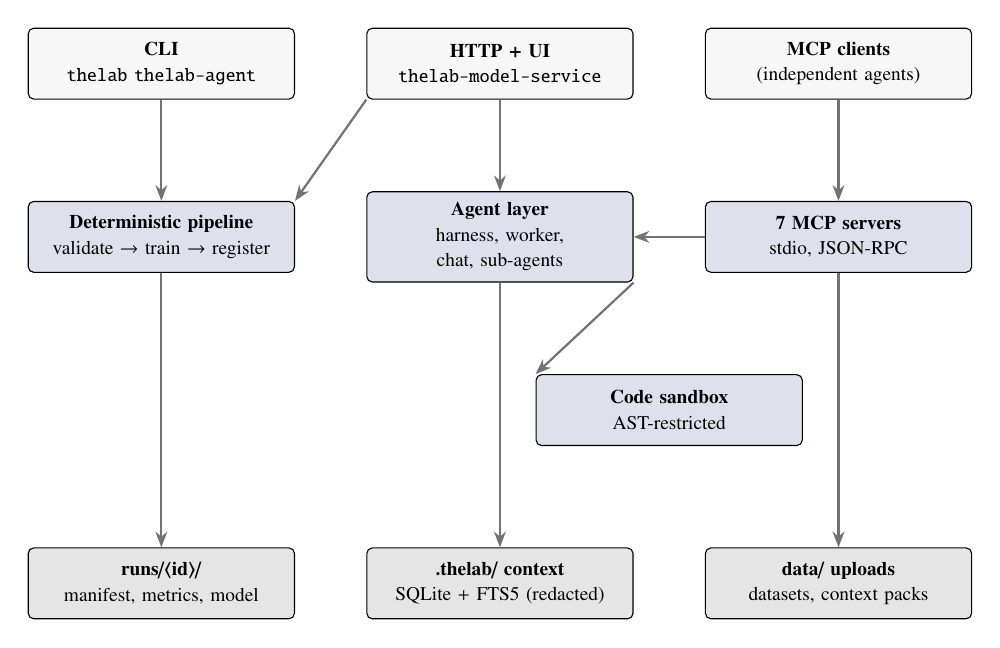
\begin{tikzpicture}[
	font=\scriptsize,
	box/.style={draw=black, rounded corners=2pt, align=center, inner sep=4pt, text width=3.1cm, minimum height=9mm},
	iface/.style={box, fill=gray97},
	core/.style={box, fill=azulUC3M!12},
	store/.style={box, fill=gray75!40},
	arr/.style={-{Stealth[length=2mm]}, thick, draw=gray45}
]
% Interfaces (row 1)
\node[iface] (cli)    at (0,4.4)    {\textbf{CLI}\\\texttt{thelab} \texttt{thelab-agent}};
\node[iface] (http)   at (4.3,4.4)  {\textbf{HTTP + UI}\\\texttt{thelab-model-service}};
\node[iface] (mcp)    at (8.6,4.4)  {\textbf{MCP clients}\\(independent agents)};
% Core (row 2)
\node[core] (pipe)    at (0,2.2)    {\textbf{Deterministic pipeline}\\validate $\rightarrow$ train $\rightarrow$ register};
\node[core] (agents)  at (4.3,2.2)  {\textbf{Agent layer}\\harness, worker, chat, sub-agents};
\node[core] (mcpsrv)  at (8.6,2.2)  {\textbf{7 MCP servers}\\stdio, JSON-RPC};
% Sandbox (row 3, col 2-3 gap)
\node[core] (sandbox) at (6.45,0)   {\textbf{Code sandbox}\\AST-restricted};
% Stores (row 4)
\node[store] (runs)   at (0,-2.2)   {\textbf{runs/\textlangle id\textrangle/}\\manifest, metrics, model};
\node[store] (ctx)    at (4.3,-2.2) {\textbf{.thelab/ context}\\SQLite + FTS5 (redacted)};
\node[store] (data)   at (8.6,-2.2) {\textbf{data/ uploads}\\datasets, context packs};
% Arrows
\draw[arr] (cli.south) -- (pipe.north);
\draw[arr] (http.south west) -- (pipe.north east);
\draw[arr] (http.south) -- (agents.north);
\draw[arr] (mcp.south) -- (mcpsrv.north);
\draw[arr] (mcpsrv.west) -- (agents.east);
\draw[arr] (mcpsrv.south) -- (data.north);
\draw[arr] (pipe.south) -- (runs.north);
\draw[arr] (agents.south) -- (ctx.north);
\draw[arr] (agents.south east) -- (sandbox.north west);
\end{tikzpicture}
\caption{\emph{thelab-mcp} architecture: three ways in (CLI, HTTP/UI, MCP) over one deterministic core; agents and the sandbox mediate non-deterministic decisions; all state lands in local, inspectable stores.}
\label{fig:architecture}
\end{figure}

The implementation is organized into ten Python packages, summarized in Table~\ref{tab:modules}; approximately 16{,}900 lines of code in total, excluding the workspace front end.

\begin{table}[H]
\centering
\caption{Module map of the \texttt{thelab} package.}
\label{tab:modules}
\small
\begin{tabular}{p{3.2cm}p{11.2cm}}
\toprule
\textbf{Package} & \textbf{Responsibility} \\
\midrule
\texttt{contracts} & Six canonical Pydantic typed contracts imported by every other package \\
\texttt{run} & Deterministic factory: validation, profiling, training, artifacts, batch, comparison, notebooks \\
\texttt{context} & SQLite + FTS5 evidence store: repository, redaction, read-only reader, indexer \\
\texttt{agents} & Provider protocol and adapters, harness, worker agent, global agents, chat agent \\
\texttt{ide} & Agentic ML IDE backend: jobs (SSE), orchestrator, datasets, cleaning, experiments, Kaggle \\
\texttt{mcp} & Seven stdio MCP servers, shared path-safety helpers, demo client \\
\texttt{sandbox} & AST-restricted subprocess for LLM-generated code \\
\texttt{model\_service} & FastAPI service and dashboard serving the three API surfaces \\
\texttt{eda} & Deterministic exploratory data analysis skill pack (six pure functions) \\
\texttt{workspace} & Path containment and SHA-256 hashing utilities \\
\bottomrule
\end{tabular}
\end{table}

\section{Typed contracts}
\label{sec:contracts}

All information exchanged between components (human, deterministic, or agentic) travels in six canonical contracts built with Pydantic \cite{pydantic2024} in strict mode (\texttt{strict=True, extra="forbid"}), so that unknown fields and automatic type conversions are rejected rather than silently accepted. This choice is the whole motive of the architecture: agents can only communicate through types the whole system already understands, which removes an entire class of integration errors.

The central contract is the run manifest, shown in Code~\ref{lst:manifest}. It records the input hash, the complete training configuration, the random seed, and the resolved dependency versions: the minimum provenance needed to reproduce and to audit a run.

\begin{lstlisting}[language=json, caption={The \texttt{RunManifest} contract (\texttt{thelab/contracts/run\_manifest.py}).}, label={lst:manifest}, style=estilo]
class RunManifest(BaseModel):
    model_config = ConfigDict(strict=True, extra="forbid")

    run_id: str
    input_hash: str                      # SHA-256 of the dataset
    training_config: dict[str, Any]
    random_seed: int
    dependency_versions: dict[str, str]
    started_at: datetime
    finished_at: datetime | None
    final_status: RunStatus              # pending|running|completed|failed|rejected
    validation_status: ValidationStatus  # pending|approved|rejected
    artifact_refs: list[ArtifactRef]
    error_summary: str | None
    task_type: Literal["classification", "regression"] | None
\end{lstlisting}

Artifact references deserve special mention. Every artifact is addressed by a \emph{relative} path and a content hash; a validator rejects absolute paths and any path containing \texttt{..} parts (Code~\ref{lst:artifactref}), making traversal attacks unrepresentable in the type system rather than just forbidden by a convention.

\begin{lstlisting}[language=json, caption={The \texttt{ArtifactRef} contract: relative paths enforced by validation.}, label={lst:artifactref}, style=estilo]
class ArtifactRef(BaseModel):
    model_config = ConfigDict(strict=True, extra="forbid")

    artifact_id: str
    artifact_type: str
    relative_path: Path    # validator rejects absolute paths and ".."
    content_hash: str      # SHA-256
    origin: str
    parent_run_id: str
\end{lstlisting}

The remaining contracts complete the vocabulary:

\begin{itemize}
	\item \texttt{TaskSpec} (an orchestrator's unit of work, with \texttt{objective}, \texttt{input\_refs}, \texttt{constraints}, and \texttt{task\_state}),
	\item \texttt{DatasetSpec} (source, expected schema, target, quality rules, privacy classification),
	\item \texttt{ModelSpec} (algorithm, hyperparameters, target metric, seed, version), and \texttt{LogEntry} (event type, tags, redacted summary, artifact references, privacy level).
	\item \texttt{ExperimentProposal} (the shape an agent's suggestion must take) extends this vocabulary with a goal, a model grid validated against the model registry, seeds, and a rationale grounded in EDA and prior runs.
\end{itemize}

\section{The deterministic pipeline}
\label{sec:pipeline}

The pipeline converts a local CSV into a registered model through a fixed sequence: \emph{validate $\rightarrow$ profile $\rightarrow$ contract $\rightarrow$ train $\rightarrow$ re-validate $\rightarrow$ register}. Each stage is a pure, testable transformation and the composition is deterministic given (dataset, model, seed). The order matters: profiling runs before training so that a dataset with silent problems (wrong types, a missing target, constant columns) fails early with a reason, instead of failing mid-training without one.

\subsection{Validation as a gate}

Input validation is needed for the pipeline to work seamlessly without errors. It checks schema conformance, data types, missing values, duplicates, target validity, and split feasibility. It is also useful when the pipeline fails, when a run is rejected (\texttt{final\_status=rejected}), all the evidence is stored in the same format as successful runs, letting agents have context about failed runs to avoid similar mistakes in the future.

\subsection{Task-type inference and the model registry}

The task type (classification or regression) is inferred from the target column (at most 20 distinct values $\Rightarrow$ classification) or can be forced explicitly. Nine model families are registered (Table~\ref{tab:models}); each entry carries its estimator class, default parameters, probability support, task type, and an optional \emph{scale guard} \texttt{max\_train\_rows}. When a configuration violates a guard (for example, \texttt{svc} on 113{,}769 rows), the run is rejected \emph{in milliseconds} instead of running for hours and exhausting memory.


\begin{table}[H]
\centering
\caption{Registered model families and their guards.}
\label{tab:models}
\small
\begin{tabular}{llll}
\toprule
\textbf{Name} & \textbf{Task} & \textbf{Estimator} & \textbf{Guard} \\
\midrule
\texttt{logistic\_regression} & classification & \texttt{LogisticRegression} & \\
\texttt{random\_forest} & classification & \texttt{RandomForestClassifier} & \\
\texttt{svc} & classification & \texttt{SVC} & $\leq$ 50{,}000 train rows \\
\texttt{sgd\_classifier} & classification & \texttt{SGDClassifier} & \\
\texttt{hist\_gradient\_boosting} & classification & \texttt{HistGradientBoosting...} & \\
\texttt{linear\_regression} & regression & \texttt{LinearRegression} & \\
\texttt{ridge} & regression & \texttt{Ridge} & \\
\texttt{random\_forest\_regressor} & regression & \texttt{RandomForestRegressor} & \\
\texttt{hist\_gradient\_boosting\_regressor} & regression & \texttt{HistGradientBoosting...} & \\
\bottomrule
\end{tabular}
\end{table}

The seed is injected into every estimator (\texttt{random\_state=seed}) and into the train/test split. Preprocessing is a fixed \texttt{StandardScaler} pipeline and metrics are computed consistently throughout runs: accuracy and macro-F1 for classification, RMSE, MAE, and $R^2$ for regression, on both train and test partitions.

\subsection{The cleaning policy}

One of the first problems was that real datasets almost never arrive clean. To make it work, the deterministic cleaning policy turns raw uploads into trainable tables while remaining fully auditable: rows with a missing target are dropped; datetime columns are parsed into numeric calendar features; categorical columns with at most 20 distinct values are one-hot encoded, while high-cardinality categoricals (e.g., 500 ticker symbols) are frequency-encoded; missing numeric values are imputed and constant columns are dropped. Every action is recorded per column in a \texttt{cleaning\_report}. The importance of the cardinality rule is quantified in Chapter~\ref{ch:results}: for example on a real 164{,}231-row financial dataset, naive one-hot encoding produced a 22~GB intermediate file, while the final cleaning policy produced 16--21~MB with the same raw data.

\subsection{Run artifacts}

Each completed (or rejected) run generates eleven artifacts in \texttt{runs/<run\_id>/}: \texttt{manifest.json}, \texttt{task\_spec.json}, \texttt{events.jsonl}, \texttt{inputs.json}, \texttt{data\_profile.json}, \texttt{dataset\_contract.json}, \texttt{training\_config.json}, \texttt{metrics.json}, \texttt{validation\_report.json}, \texttt{model.joblib}, and \texttt{model\_card.md}. This directory is the unit of evidence for the whole system: MCP servers, the registry, the UI, and the context indexer all read from it, and Annex~B reproduces a real manifest.

\section{The context store}
\label{sec:contextstore}

The context store is \emph{thelab-mcp}'s memory: a local SQLite database with an FTS5 full-text index, designed around four properties.

\begin{enumerate}
	\item \textbf{Redaction at write time.} To avoid possible sensitive information leakage, twelve ordered regular-expression families strip private key blocks, bearer tokens, GitHub personal access tokens, Google/AWS/Slack API keys, \texttt{sk-} keys, passwords, and secret-valued environment variables, replacing matches with \texttt{[REDACTED]} before anything is persisted.
	\item \textbf{Content-addressed idempotence.} Every entry carries a SHA-256 \texttt{content\_hash} over its canonical JSON content; re-indexing the same event has no effect, and a mismatched hash on the same event id raises an error rather than corrupting the store.
	\item \textbf{Privacy levels.} Entries are classified \texttt{public}/\texttt{internal}/\texttt{restricted}/\texttt{secret}; readers default to the first two, and the restricted tiers require explicit override.
	\item \textbf{Read-only retrieval.} The reader opens the database with \texttt{mode=ro} and \texttt{PRAGMA query\_only=ON}, so retrieval cannot mutate evidence, a property RQ3 asserts byte-for-byte.
\end{enumerate}

Search is keyword-based (SQLite FTS5, results ranked by relevance) over the redacted summaries, with structured filters for run id, tags, event type, and time range. Entries arrive from three sources: the JSONL event log of runs, agent session summaries sent through the \texttt{context\_write} MCP server (redacted on arrival), and the Kaggle ingestion, which adds one context pack
per dataset.


\section{The MCP surface}
\label{sec:mcp}

Seven MCP servers expose the factory to independent clients over \emph{stdio} --- chosen deliberately for a local-first system: servers run as plain child processes with no network surface, no ports, and no authentication layer to configure, and the single-job split lets a client connect only to what it needs:

\begin{itemize}
	\item \texttt{data\_catalog}: what datasets exist, with their profiles and contracts.
	\item \texttt{model\_registry}: the approved models, and inference with them. This is the RQ2 surface.
	\item \texttt{workspace}: the runs, their manifests, and their artifacts.
	\item \texttt{context}: search over the evidence store (read-only).
	\item \texttt{context\_write}: one tool to append agent session summaries, redacted on arrival.
	\item \texttt{eda}: the six deterministic EDA skills (missing values, correlations, class balance, outliers, leakage suspects, feature types).
	\item \texttt{agent}: orchestration, spawning sub-agents, and training jobs, always behind the approval gate.
\end{itemize}

Table~\ref{tab:mcpservers} lists the complete tool set (32 tools). All seven servers share the same safety basics: run ids are checked against traversal and dot-entries, every answer uses the same \texttt{\{ok, data\}} / \texttt{\{ok, error\}} format, and every tool declares a bounded schema (for example, queries of at most 200 characters) that rejects malformed calls before they run.

\begin{table}[H]
\centering
\caption{The seven MCP servers and their tools.}
\label{tab:mcpservers}
\small
\begin{tabular}{p{3.2cm}p{10.3cm}}
\toprule
\textbf{Server} & \textbf{Tools} \\
\midrule
\texttt{data\_catalog} & \texttt{list\_datasets}, \texttt{get\_data\_profile}, \texttt{get\_dataset\_contract} \\
\texttt{model\_registry} & \texttt{list\_models}, \texttt{get\_model\_manifest}, \texttt{get\_model\_card}, \texttt{get\_model\_metrics}, \texttt{predict} \\
\texttt{workspace} & \texttt{list\_runs}, \texttt{get\_run\_manifest}, \texttt{list\_run\_artifacts}, \texttt{get\_artifact}, \texttt{read\_model\_card} \\
\texttt{context} (read-only) & \texttt{get\_context\_status}, \texttt{get\_context\_entry}, \texttt{search\_context} \\
\texttt{context\_write} & \texttt{append\_session\_summary} (server-side redaction) \\
\texttt{eda} & \texttt{missing\_profile}, \texttt{correlation\_hints}, \texttt{class\_balance}, \texttt{outlier\_scan}, \texttt{leakage\_suspects}, \texttt{feature\_types} \\
\texttt{agent} & \texttt{orchestrate\_experiment}, \texttt{run\_full\_journey}, \texttt{continue\_journey}, \texttt{get\_journey\_status}, \texttt{spawn\_subagent}, \texttt{run\_deterministic\_skill}, \texttt{run\_training\_job}, \texttt{get\_job\_status}, \texttt{log\_agent\_activity} \\
\bottomrule
\end{tabular}
\end{table}

The main separation of powers is carried out by three of the servers. The idea behind it is simple: the ability to read evidence is separated from the
ability to change it, and the ability to use a model is separated from the ability to train one. An external agent can therefore look at everything the system recorded, but it can only modify the record through guarded doors.

The read-only \texttt{context} server is the first half. It gives any client search over the evidence, with no write path at all: whatever an agent learns from it, it cannot rewrite or delete. The \texttt{context\_write} server is the guarded door in the other direction. It accepts session summaries only after the same redaction pipeline the store itself uses, so an agent can add to the record but cannot bypass the redaction. Finally, the \texttt{model\_registry} server is the RQ2 surface: \texttt{list\_models} and \texttt{predict} expose approved models with no reference to the training code that produced them, so inference can be done by an agent that has no idea how the model was built. And because serving is gated by validated state, a model that never passed validation simply does not exist for this server.

\section{The agent layer}
\label{sec:agents}

\subsection{Provider abstraction}

Every LLM interaction goes through one small interface. The system asks a provider to complete a conversation, and the provider answers with either text or a tool call. Four providers implement this interface: a scriptable \texttt{MockProvider} (used by the entire test suite, so the system is fully testable with zero network access), \texttt{OllamaProvider} for local models \cite{ollama2024}, \texttt{OpenAICompatProvider} for the de-facto \texttt{/v1/chat/completions} standard, and \texttt{OpenRouterProvider}. Switching providers is configuration, not code, so the abstraction layer follows the industry-standard protocol itself. This abstraction is what makes the provider experiments of Chapter~\ref{ch:results} possible: the same pipeline runs against a reasoning cloud model, a non-reasoning cloud model, or a fully offline local one, without a single code change.

\subsection{The harness and grounding}

The \texttt{AgentHarness} runs a bounded tool loop (8 steps by default) over the MCP server connections. It discovers the tools, pins a read-only
allowlist, and \emph{grounds} every answer, checking each statement against the saved run files before accepting it. Grounding lives in one shared module (\texttt{thelab/agents/grounding.py}), so the rules are the same for the harness, the chat agent, and the global agents. A claim counts as grounded only when the run ids it cites really exist and the metrics it quotes match the recorded \texttt{metrics.json} values (within a tolerance of $10^{-3}$, across ten metric keys). If a check fails, the harness returns a structured refusal (\texttt{grounding\_failure}) instead of a plausible-looking answer. Without this check, a confident answer citing a metric that does not exist would be indistinguishable from a correct one. With it, overconfidence becomes a refusal the record shows.

\subsection{Worker agent and proposals}

The \texttt{WorkerAgent} turns goals into \texttt{ExperimentProposal} objects: it feeds the provider a prompt seeded with deterministic EDA results (missing values, class balance, feature types, inferred task type) and the metrics of the last three completed runs on the same dataset and target, so that proposals are grounded in evidence by construction. To make things work and avoid problems at runtime, the LLM provider's output passes through a conservative JSON-repair ladder (markdown-fence stripping, Python triple-quoted-string conversion, trailing-comma and single-quote fixes, unquoted-key quoting) that maintains the required format. If it fails, a deterministic fallback proposal is carried out instead. The worker \emph{never} executes. Proposals are persisted by a \texttt{ProposalStore}, and every path that turns a proposal into training must pass the approval gate (Section~\ref{sec:approvalgate}).

\subsection{The approval gate}
\label{sec:approvalgate}

Approval is enforced and carried out in exactly one place, the module \texttt{approval.py} in \texttt{thelab/agents/}. No other piece of agentic code can approve anything, so there is only one door to check.

\begin{itemize}
	\item \textbf{Agent-initiated flows} (an MCP client asking for orchestration) return \texttt{awaiting\_approval} by default. An agent cannot silently execute training. Auto-approval exists only behind an explicit environment flag, and even then it is recorded as \texttt{auto:\textlangle principal\textrangle}, so the record shows it was not a human decision.
	\item \textbf{User-initiated flows} (a CLI or UI experiment run) carry the initiator's recorded mandate. The deterministic stages are approved automatically as \texttt{auto:}\allowbreak{}\texttt{experiment:}\allowbreak{}\texttt{\textlangle id\textrangle}, so the audit trail shows who started the experiment and that no human reviewed that specific proposal.
	\item \textbf{Rejection is final.} A rejected proposal can never be executed. The gate refuses it outright, closing a loophole in which an approval action could overwrite a rejection.
\end{itemize}

\subsection{Role agents and the orchestrator}

Three role-specialized agents (\texttt{EDAAnalyst}, \texttt{FeatureEngineer}, \texttt{ModelSelector}) participate in an orchestrated experiment, each with a \emph{distinct system-prompt contract} (\texttt{ROLE\_SYSTEM\_PROMPTS}) that fixes its identity, scope, and output format for the stage. The \texttt{ExperimentOrchestrator} sequences the stages (EDA $\rightarrow$ feature engineering $\rightarrow$ model selection $\rightarrow$ approved batch training). Aditionally it applies user feedback to all three stage interpretations and to the proposal goal, emits stage events, and when a real provider is configured, it adds LLM interpretations per stage over its deterministic output. The interpretations are persisted alongside the results as searchable context, that can be used by the \emph{sub-agents} spawned by the \texttt{ExperimentOrchestrator} . If the provider fails, the pipeline continues deterministically, so interpretation never blocks execution.  (Section~\ref{sec:agentmetrics}).

\subsection{The agentic round}
\label{sec:agenticround}

The agentic round is the system's \emph{grounded autonomy} mechanism and the multi-orquestration claims. It is an additional exploration stage that runs \emph{after} the deterministic batch, starts from the artifacts that batch produced, and validates everything deterministically before it can affect training. A context pack (EDA brief, baseline metrics, prior-run evidence, and user feedback, assembled without any LLM) grounds three sequential roles: Each role can be assigned its own LLM provider (per-stage model assignment): the round's configuration accepts a role-to-provider mapping, so a mixed team --- for example, a fast analyst, a reasoning feature-engineer, and a cheap selector --- runs through the same gated pipeline. Every stage records its assigned model and, where the provider reports them, per-stage token counts and cost, making the role-to-model assignment a measured rather than assumed choice. The loop that wraps these rounds is recorded as a typed evidence artifact: a per-dataset generation ledger storing the deterministic baseline, every round (validity, mode, entries, the exact prompts sent to each stage, and per-stage token counts and cost), the absorption decision with its replay proof, and the champion configuration (model, seed, hyperparameters). The ledger is what makes the loop auditable after the fact: every claim about an absorption resolves to a recorded entry.

\begin{enumerate}
	\item \textbf{Analyst}: reads the context store and EDA evidence through read-only MCP tools to explain \emph{why} the baseline performs as it does and what to try next; output is a typed findings brief (findings, opportunities, risks) with deterministic fallback.
	\item \textbf{FeatureEngineer}: generates one pandas transform that executes \emph{only} inside the sandbox; the transformed artifact is then checked by a deterministic post-validator (shape and schema, target intactness, constant-feature rejection, the at-decision-time leakage policy) before it may reach training, and metrics are always recomputed by the deterministic factory: sandbox output is never trusted.
	\item \textbf{ModelSelector}: proposes training configurations beyond the fixed deterministic grid, validated against the model registry and persisted through the proposal store behind the human-default approval gate.
\end{enumerate}

Execution of an approved round runs as a tracked background job (stage events surfaced in the UI, cooperative cancellation), and the round ends with a comparison record (best agentic versus best deterministic, with signed metric deltas, validity rates, and rejections) persisted alongside the run artifacts and indexed into the context store. The round is the instrument of RQ4--RQ6 (Section~\ref{sec:exp-agentic}).

\subsection{The chat agent}

The grounded chat agent (\texttt{POST /agent/chat}, and the UI chat drawer) is the user-facing intelligence of the workspace. It runs a bounded loop (12 steps) over eight tools: \texttt{search\_context}, \texttt{list\_recent\_runs}, \texttt{get\_run\_summary}, \texttt{dataset\_eda}, \texttt{get\_dataset\_context}, \texttt{clean\_dataset}, \texttt{run\_python} (sandboxed; dataset exposed read-only as \texttt{dataset.csv}), and \texttt{propose\_experiment}. Every turn is persisted to the context store as a redacted session summary. The agent's self-description is worth quoting because it states the design in first person: it reads context packs, runs deterministic EDA, explores data hands-on in the sandbox, \emph{proposes} experiments (``I never train models myself''), and searches memory: the human approves and the factory executes.

\subsection{Global agents}

Two additional agents complete the layer: a \texttt{Researcher} that answers questions strictly from allowlisted artifacts with claim-id citations, and a \texttt{DiagnosisAgent} that triages failed runs into approved or rejected follow-ups. Both run over the same harness and provider abstraction.

\section{Experiment lifecycle}
\label{sec:lifecycle}

Orchestrated experiments are first-class state machines, persisted as JSON by an \texttt{ExperimentStore}. Persistence is what makes the machine trustworthy: a crash or restart does not lose the experiment, any state can be inspected later like any other evidence, and the JSON file itself is stored in the same evidence format as everything else. Figure~\ref{fig:lifecycle} shows the states. Two transitions deserve note: \texttt{completed} may cycle back through \texttt{iterating} when the user sends feedback (``focus on tree models''), producing a new planning phase informed by the previous results; and \texttt{cancelled} is reachable from \texttt{training} through cooperative cancellation: jobs check a flag between stages and between models, so a cancel request takes effect promptly without orphaning partial runs.

\begin{figure}[H]
\centering
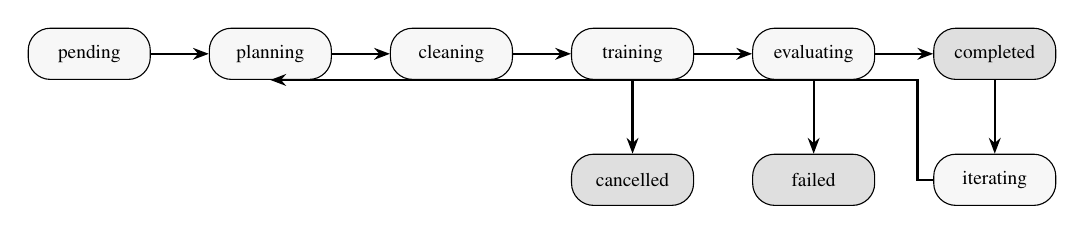
\begin{tikzpicture}[
	font=\scriptsize,
	state/.style={draw=black, rounded corners=8pt, align=center, inner sep=3pt, minimum height=6.5mm, minimum width=15.5mm, fill=gray97},
	terminal/.style={state, fill=gray75!50},
	arr/.style={-{Stealth[length=2mm]}, thick}
]
\node[state] (pending) at (0,0) {pending};
\node[state] (planning) at (2.3,0) {planning};
\node[state] (cleaning) at (4.6,0) {cleaning};
\node[state] (training) at (6.9,0) {training};
\node[state] (evaluating) at (9.2,0) {evaluating};
\node[terminal] (completed) at (11.5,0) {completed};
\node[terminal] (cancelled) at (6.9,-1.6) {cancelled};
\node[terminal] (failed) at (9.2,-1.6) {failed};
\node[state] (iterating) at (11.5,-1.6) {iterating};
\draw[arr] (pending) -- (planning);
\draw[arr] (planning) -- (cleaning);
\draw[arr] (cleaning) -- (training);
\draw[arr] (training) -- (evaluating);
\draw[arr] (evaluating) -- (completed);
\draw[arr] (training) -- (cancelled);
\draw[arr] (evaluating) -- (failed);
\draw[arr] (completed.south) -- (iterating.north);
\draw[arr] (iterating.west) -- ++(-2mm,0) |- (planning.south);
\end{tikzpicture}
\caption{Experiment lifecycle state machine (persisted per experiment).}
\label{fig:lifecycle}
\end{figure}

Execution runs through a background \texttt{JobManager} with server-sent events (SSE) streaming per-stage and per-model progress to the UI; every event is also appended to the run's \texttt{events.jsonl}, so the live view and the post-hoc evidence are the same data. Approved agentic rounds (Section~\ref{sec:agenticround}) execute as a further tracked job stage after the deterministic batch, streaming per-agent events through the same channel.

\section{The workspace UI}
\label{sec:ui}

The web workspace (React 18 + TypeScript + Vite, hand-rolled CSS token set, Recharts for charts) is organized as a five-view experiment-centric layout with a deliberate visual grammar: blue for the deterministic side, purple for the agentic side. Two folders structure the sidebar. \emph{Deterministic} holds the Data view (upload of CSV and parquet files, Kaggle import with automatic context-pack build, sortable preview with horizontal scroll, EDA card grid, cleaning with audit report) and Model Lab (deterministic try-all job with per-model SSE and comparison bars). \emph{Agentic} holds the Experiments view (plan, run with live sub-agent stage pipeline, history with feedback; proposals live inside the Experiments flow, where approving one launches a first-class tracked experiment with the full stage pipeline and best-run summary). A mini-dock hosts the Global Agent chat drawer and the Admin views (model registry with metrics/artifacts/predict/evidence tabs, context search with sessions, sandbox playground, an MCP server inventory panel, and the generated-notebook viewer). The chat drawer streams per-tool progress, renders markdown, exposes usage/token/time telemetry per exchange, accepts style and role directives, supports inline proposal approval, and persists the conversation across open/close, with every exchange indexed into the context store. Dataset context is shared across views, so the dataset being explored in Data is the one proposed upon in Experiments. The design goal is stated as one sentence in the project notes: \emph{a workspace a human actually wants to use}, with the pipeline visible rather than hidden, a glass box and not a black box.

A note on provenance of this decision: the first UI was deliberately dependency-free vanilla JavaScript; the rework to React+Vite was an explicit, documented break of that constraint in exchange for maintainability and charting ergonomics: recorded here as an example of the project's willingness to revise its own rules when evidence favored it.

\begin{figure}[H]
\centering
\resultslot[5.5cm]{Screenshot slot A: Data view: upload, preview, EDA modules (missing values, distributions, correlations) and the cleaning report, in the deterministic (blue) folder.}
\caption{Workspace UI: the deterministic Data view (screenshot pending).}
\label{fig:ui-data}
\end{figure}

\begin{figure}[H]
\centering
\resultslot[5.5cm]{Screenshot slot B: Experiments view: live stage pipeline (Plan $\rightarrow$ Clean $\rightarrow$ Train $\rightarrow$ Evaluate, plus the agentic round stage), per-agent cards with LLM interpretations, per-model SSE progress, and History with feedback.}
\caption{Workspace UI: the agentic Experiments view (screenshot pending).}
\label{fig:ui-experiments}
\end{figure}

\section{Safety and security model}
\label{sec:safety}

Three mechanisms define the safety model; Table~\ref{tab:safety} summarizes their guarantees and their honest limits.

\begin{table}[H]
\centering
\caption{Safety mechanisms: guarantees and limits.}
\label{tab:safety}
\small
\begin{tabular}{p{3.1cm}p{6.2cm}p{5.1cm}}
\toprule
\textbf{Mechanism} & \textbf{Guarantee} & \textbf{Documented limit} \\
\midrule
Path containment & Workspace-relative paths only; \texttt{resolve()+relative\_to} blocks traversal and symlinks; \texttt{ArtifactRef} validates relativity & Absolute paths may leak in some library error strings (MAJ-01, open) \\
Code sandbox & Import whitelist (22 modules), 14 blocked builtins, 13 blocked AST node types (lambdas deliberately allowed for pandas idioms), dunder guard, 2~GB RLIMIT, 30~s timeout, output caps & Compute isolation only; no OS-level filesystem confinement (BLK-01, open). The trade-off is deliberate: a local-first, single-user tool avoids requiring container runtimes on the host, and every sandbox artifact is treated as untrusted and re-validated in the parent process \\
Approval gate & Every path from proposal to training passes one chokepoint; agent-initiated flows default to \texttt{awaiting\_approval}; rejected proposals are unexecutable & Social, not cryptographic: the principal is recorded (\texttt{auto:} mandates included), not authenticated \\
\bottomrule
\end{tabular}
\end{table}

The sandbox deserves elaboration because it executes LLM-generated code. It spawns a fresh interpreter for every execution, speaking a JSON protocol over stdin/stdout, forcing a non-interactive matplotlib backend, and enforcing its policy in three layers. The first layer is a static AST check that rejects forbidden constructs before execution: class definitions, async constructs, dynamic \texttt{type()} calls, and others. Lambdas are deliberately \emph{allowed}. The RQ5 spike proved that blocking \texttt{ast.Lambda} is incompatible with pandas-idiomatic code such as \texttt{groupby().transform(lambda s: ...)}, and a lambda cannot import, access blocked builtins, or escape scope, because \texttt{global} and \texttt{nonlocal} remain blocked. The second layer is an import hook that re-enforces the whitelist at runtime; the \texttt{inspect} module is deliberately excluded, after an audit finding showed it could recover unfiltered builtins. The third layer is compute limits: memory (2~GB, raised from 512~MB after measuring the address space pandas~3 needs for its shared libraries), wall-clock time, and output size. The hardening approach follows secure-development guidance on supply-chain and capability scoping \cite{openssf2024}, and it is aligned with the emerging MCP security literature: the OWASP MCP Security Cheat Sheet \cite{owasp2025mcp}, the NSA's security guidance for MCP deployments \cite{nsa2025mcp}, the OWASP LLM risk taxonomy (which treats unrestricted code execution and excessive agency as first-class threat classes) \cite{owasp2024llm}, and the academic analyses of MCP's attack surface \cite{zhang2026breakingprotocol,hou2026mcplandscape}. An adversarial security audit (revisited in Section~\ref{sec:lessons}) found and fixed two escape chains and documented the remaining filesystem-confinement gap with a proof of concept. That is why this thesis describes the sandbox as providing \emph{compute isolation}, not confinement.

\subsection{Alternatives considered}
\label{sec:alternatives}

Three architectural alternatives were explicitly evaluated and set aside, a record kept here because it delimits the novelty claim:

\begin{itemize}
	\item \textbf{Orchestration frameworks (Airflow, LangGraph, AutoGen) as the core.} Rejected: an external orchestrator competes with the hand-rolled orchestration layer that is itself the thesis's object of study, diluting the claim. Frameworks remain the comparison baseline of Table~\ref{tab:frameworks}.
	\item \textbf{A workflow/data-transformation engine (dbt) and a warehouse (Snowflake/\allowbreak{}BigQuery) as the data layer.} Considered and deferred: the fit is genuine (a transformation module wrapped as an MCP tool is exactly the ``capability = MCP module'' pattern), but migrating the evidence layer from local SQLite/files to a warehouse conflicts with the local-first constraint that defines the system; recorded as future work for organizational deployments.
	\item \textbf{A vector-database memory layer (RAG) over the context store.} Deferred by explicit descope decision (Section~\ref{sec:process}): the keyword FTS5 store preserves verifiability; semantic retrieval is future work (Section~\ref{sec:futurework}).
\end{itemize}

\chapter{Implementation}
\label{ch:implementation}

This chapter describes how the design of Chapter~\ref{ch:design} is realized: the technology stack and repository layout (Section~\ref{sec:stack}), reproducibility engineering (Section~\ref{sec:reprowork}), the three usage surfaces with working examples (Section~\ref{sec:surfaces}), Kaggle ingestion (Section~\ref{sec:kaggle}), quality assurance (Section~\ref{sec:quality}), and the development process itself (Section~\ref{sec:process}).

\section{Technology stack and repository layout}
\label{sec:stack}

The stack was chosen for strong typing, determinism, and local operation. Python 3.11+ is the implementation language; Pydantic~v2 enforces the contracts; pandas and scikit-learn \cite{pedregosa2011sklearn} provide the data and model layers; the official MCP SDK \cite{mcp2024spec} serves the seven stdio servers; FastAPI and Uvicorn serve the HTTP surface \cite{fastapi2024}; kagglehub ingests public datasets \cite{kagglehub2024}; and SQLite/FTS5 \cite{sqlite2024fts5} backs the context store. The workspace front end is React 18 + TypeScript built with Vite and served as static files by the same FastAPI process, so the entire system runs as a single local service. Table~\ref{tab:stack} lists the pinned core dependencies.

\begin{table}[H]
\centering
\caption{Core dependencies (versions pinned in \texttt{requirements.lock}).}
\label{tab:stack}
\small
\begin{tabular}{llp{7.6cm}}
\toprule
\textbf{Dependency} & \textbf{Role} & \textbf{Why this one} \\
\midrule
pydantic ($\geq$2) & Contracts & Strictly typed models with validation and the contracts backbone. \\
pandas ($\geq$2) & Dataframes & Standard tabular layer \cite{mckinney2010pandas}, profiling and cleaning. \\
scikit-learn ($\geq$1.4) & Models & Nine deterministic estimators and the \texttt{random\_state} discipline \\
mcp ($\geq$1.6) & Protocol & Official SDK for stdio servers and clients \\
fastapi / uvicorn & HTTP & Async service and SSE streaming for job events \\
kagglehub & Ingestion & First-party Kaggle adapter for public datasets \\
pyarrow & Parquet & Future-proof columnar I/O support \\
matplotlib & Figures & Thesis evidence generation (validity charts, comparison plots) \\
\bottomrule
\end{tabular}
\end{table}

The repository follows a conventional Python layout. The package tree maps one-to-one onto the responsibilities of Table~\ref{tab:modules} (packages). The workspace front end lives in \texttt{web/}. Every runtime output lands under the user's workspace (\texttt{runs/}, \texttt{data/}, \texttt{proposals/}, \texttt{.thelab/}) with persisted references for context searching.

\begin{lstlisting}[language={}, caption={Repository layout (top level, abridged).}, label={lst:layout}, style=cli]
thelab/                  # implementation (10 packages, ~16k LOC)
  contracts/ run/ context/ agents/ ide/ mcp/ sandbox/
  model_service/ eda/ workspace/
  agents/approval.py    # single approval chokepoint
  agents/grounding.py   # shared claim verification
  ide/agentic_round.py  # grounded-autonomy role loop; per-stage provider assignment (stage_providers) + token/cost telemetry
web/                     # React + TS workspace (Vite build)
tests/                   # 58 test files, 546 test functions
scripts/                 # evaluate_thesis.py, demo_defense.sh, harvest_findings.py,
                         #   probe_model_latency.py, generate_evidence.py, build_ui.sh
examples/                # fixtures, batch configs, Kaggle experiment
docs/                    # user/CLI/API guides, thesis map, legacy records
runs/ data/ proposals/ .thelab/   # runtime workspace (user-local)
thesis/evidence/         # thesis evidence pack (tables, figures, snapshots)
\end{lstlisting}

\section{Reproducibility engineering}
\label{sec:reprowork}

Reproducibility was one of the main goals and is engineered into the pipeline. The four mechanisms that cooperate to make it true are:

\begin{enumerate}
	\item \textbf{Seed injection.} The seed is a mandatory argument of every run, injected into the estimator (\texttt{random\_state}) and \texttt{build\_estimator} refuses to construct an estimator without it.
	\item \textbf{Manifest provenance.} The manifest records the input dataset hash, the full training configuration, the seed, and the resolved dependency versions (Python, pydantic, pandas, scikit-learn, numpy, joblib), captured automatically at run time and not maintained by hand.
	\item \textbf{Lockfile.} \texttt{requirements.lock} pins the environment. The documented install path builds the virtual environment from this file, so the recorded dependency versions can be reproduced in practice (Section~\ref{sec:limitations}).
	\item \textbf{Generated notebooks.} Every completed run can produce a reproducible research notebook artifact (\texttt{report.}\allowbreak{}\texttt{ipynb}, generated on demand over \texttt{GET /runs/}\allowbreak{}\texttt{\{id\}/}\allowbreak{}\texttt{notebook}). The notebook opens with a title and manifest summary, loads the dataset, and includes a reproduce cell that invokes the pipeline with the exact recorded parameters. It also shows the metrics and validation results, indexes the artifacts, and adds the sub-agent findings when present. It is built as standards-compliant nbformat JSON without new dependencies, and is viewable read-only in the UI.
\end{enumerate}

\section{Three ways in: CLI, Python API, HTTP}
\label{sec:surfaces}

The same pipeline is reachable in three different ways. The CLI (Code~\ref{lst:cli}) is the primary surface for scripting and the reference for documentation.

\begin{lstlisting}[language=bash, caption={Reproducible training and prediction from the CLI.}, label={lst:cli}, style=cli]
# Train one model deterministically
thelab run model --dataset examples/iris.csv --target species \
  --model logistic_regression --seed 42 --output runs

# Output:
# Run completed: run-20260814-222154-a5a01046
#   Model: logistic_regression   Seed: 42
#   Test accuracy: 1.000000      Test macro F1: 1.000000

# One-off prediction from an approved run
thelab predict --run-id <run_id> --features '5.1,3.5,1.4,0.2'

# Index and search the local evidence store
thelab context index --source .thelab/local-logs/agent-events.jsonl
thelab context search "reproducibility" --limit 10

# Agent CLI: worker mode proposes an experiment (EDA-grounded)
thelab-agent --mode worker --dataset examples/iris.csv --target species \
  --model-grid logistic_regression,random_forest --seeds 42,43 \
  --provider openrouter
\end{lstlisting}

The Python API offers the same capabilities to notebooks and scripts (Code~\ref{lst:python}): a low-level \texttt{run\_model} and \texttt{try\_all\_models}, and a high-level \texttt{thelab.quick}.

\begin{lstlisting}[language=python, caption={Python API: deterministic run, try-all comparison, and a proposal from a notebook.}, label={lst:python}, style=estilo]
from thelab.quick import experiment, compare

exp = experiment("examples/iris.csv", target="species", model="svc")
print(exp.metrics)                       # recorded metrics
print(exp.predict([5.1, 3.5, 1.4, 0.2])) # inference from the run

for e in compare("examples/iris.csv", target="species"):
    print(e.model, e.metrics.get("test_accuracy"))

# Agent proposals are importable too -- deterministic fallback, no LLM needed
import asyncio
from thelab.agents.mock import MockProvider
from thelab.agents.worker import WorkerAgent
from thelab.ide.proposals_api import approve_and_run_proposal

worker = WorkerAgent(provider=MockProvider([]), servers=[],
                     proposals_dir="proposals")
p = asyncio.run(worker.propose(goal="Predict species",
                               dataset="examples/iris.csv",
                               target="species",
                               model_grid=["logistic_regression"],
                               seeds=[42]))
outcome = approve_and_run_proposal(p.proposal_id, principal="notebook")
\end{lstlisting}

The HTTP surface serves the UI and a JSON API. Every answer uses the same \texttt{\{ok, data\}} format, so all clients read responses the same way (Code~\ref{lst:http}). Long operations run as background jobs, not inside the request. Training jobs stream their progress live, and experiment jobs move from stage to stage, so a cancel request is cooperative and takes effect at the next safe boundary instead of interrupting a model mid-training. One limitation is documented here: a long synchronous model fit can briefly hold other service traffic (Section~\ref{sec:limitations}).


\begin{lstlisting}[language=bash, caption={HTTP surface: training and inference via the local service.}, label={lst:http}, style=cli]
thelab-model-service --host 127.0.0.1 --port 8000

curl -s -X POST localhost:8000/train -H 'Content-Type: application/json' \
  -d '{"dataset_id": "fixtures/iris.csv", "target": "species",
       "model": "logistic_regression", "seed": 42}'

curl -X POST http://127.0.0.1:8000/predict -H "Content-Type: application/json" \
  -d '{"run_id": "run-20260829-...", "features":
       [{"sepal_length": 5.1, "sepal_width": 3.5,
         "petal_length": 1.4, "petal_width": 0.2}]}'
\end{lstlisting}

Alongside these three, an external agent can use the whole factory through the MCP servers of Table~\ref{tab:mcpservers}. It can search the stored context and use the provided tools via the MCP contracts. To prove it works, the repository includes a small demo client that connects to the servers, discovers their tools, and calls them, knowing nothing about the system beyond the protocol itself:

\begin{lstlisting}[language=bash, caption={MCP smoke tests over stdio.}, label={lst:mcpdemo}, style=cli]
thelab-mcp-demo model_registry --run-id <run_id>  # list_models, card, predict
thelab-mcp-demo data_catalog  --run-id <run_id>   # datasets, profiles, contracts
thelab-mcp-demo context                           # search the evidence store
\end{lstlisting}

The positioning rule of thumb documented in the user guide: \emph{use the UI to explore, the CLI to automate, MCP when another agent needs the factory}.

\section{Kaggle ingestion and context packs}
\label{sec:kaggle}

Public data is a first-class input. From a Kaggle slug, the ingestion path (Code~\ref{lst:kagglecli}) downloads the dataset into \texttt{data/uploads/} through kagglehub (the only networked step and always an explicit user action). It then fetches the dataset's public page context (description, tags, and file metadata, parsed from the page's embedded state), merges it with the local profile (shape, dtypes, head), and saves the merged \emph{context pack} next to the CSV (\texttt{<name>.kaggle.json}). The pack is indexed into the context store as a searchable event and exposed to the chat agent through the \texttt{get\_dataset\_context} tool, so proposals are grounded in the dataset's own documentation: for example, ordinal encodings documented on the Kaggle page become part of the agent's evidence, providing useful additional context alongside the raw dataset, so agents can perform a better job.

\begin{lstlisting}[language=bash, caption={Kaggle ingestion via CLI.}, label={lst:kagglecli}, style=cli]
thelab ingest kaggle pavansubhasht/ibm-hr-analytics-attrition-dataset
# -> downloads CSV to data/uploads/, builds + indexes the context pack
\end{lstlisting}

\section{Testing and quality assurance}
\label{sec:quality}

Quality is enforced by four automated layers that run before any change is considered complete to avoid breaking the application code:

\begin{lstlisting}[language=bash, caption={The four quality gates.}, label={lst:gates}, style=cli]
.venv/bin/ruff check thelab tests scripts        # lint (E,F,I,UP,W,B)
.venv/bin/mypy thelab                            # static types
.venv/bin/python -m pytest tests/ -q             # 546 tests
PATH=.venv/bin:$PATH python scripts/evaluate_thesis.py   # RQ1-RQ6 (mock provider)
\end{lstlisting}

The test suite covers every package at unit level and exercises the full stack end-to-end against the mock provider, so the whole system is testable
with zero network access and zero token cost. It includes a real-data hardening suite that replays the S\&P-scale scenarios, the largest recorded
dataset, to make sure the cleaning policy and scale guards keep working at that size. It also includes a suite that tests the thesis evaluator itself as well as different tests that verify the approval boundary end to end (proposal, approve, batch, runs), the sandbox policy against adversarial inputs, the context store's immutability under reads, and the MCP contract of all seven servers. Every named suite can be found in \texttt{tests/}:
\texttt{test\_real\_data\_hardening.py} (S\&P-scale hardening), \texttt{test\_thesis\_eval.py} (evaluator), \texttt{test\_agents\_approval.py} (approval boundary), \texttt{test\_sandbox.py} (adversarial sandbox inputs), and \texttt{test\_context\_reader.py} (byte-identical reads), with the MCP contract of each server covered in its own file, such as \texttt{test\_mcp.py}.

\section{Development process}
\label{sec:process}

The project development was carried out in seven stages, P0 to P6 (see the README.md and ROADMAP.md). Each stage was subdivided into implementation
slices, tested before acceptance, so the application code did not break and the development process did not slow down. Additionally, each stage, when
finished, was audited with the help of a custom coding audit agent, which stored the findings into a markdown file to harden the application code,
adding patches and fixing bugs.

The seven stages, in order, were the following.

\begin{description}
	\item[P0, the local-first data-to-model factory.] The deterministic core was the first thing built. It included the typed contracts, the training pipeline, four read-only MCP servers, the context store, and the automated RQ1--RQ3 evaluator. The motivation was that the first usable milestone had to work without a UI, an LLM, or network access.
	\item[P1, the agentic layer.] Intelligence was added on top of that core. This stage brought the provider protocol with its first adapters, the agent harness, the worker agent with experiment proposals, the EDA skill pack, and a cross-domain benchmark, all following one idea, agents propose and the pipeline executes.
	\item[P2, the agentic ML IDE.] In this stage the factory became usable on real data. Dataset upload with EDA and cleaning, background jobs with live progress, the code sandbox, and agent orchestration, as well as a hardening phase that added the cleaning policy, scale guards, and cooperative cancellation.
	\item[P3, multiagentic features.] The multi-agent claim became real and tangible in this stage. The grounded chat agent could run sandboxed code, ingest Kaggle data with context packs, and generate notebooks. The first multi-Kaggle proof experiment on three public datasets was also carried out on this stage, landing the first results that surpassed the deterministic model baseline.
	\item[P4, the workspace rework.] The five-view React user interface (UI) was done on this stage, the idea behind was to have a user friendly environment that a human would actually want to use besides from the CLI and scripts. In this stage an experiment was also carried out that compared local vs cloud LLM models over the created architecture.
	\item[P5, grounded autonomy.] In this stage the goal was to expand the multi-agentic features and to generate better and more efficient agent responses overall. Grounded context, per-role agent prompts, the approval gate and the RQ4--RQ6 instrumentation were built and measured in this stage.
	\item[P6, the continuous working loop.] Finally, the loop was closed. A multi-domain ratchet loop was done over ten datasets. It compared the metrics achieved by the deterministic pipeline vs the agentic expanded pipeline. If the agent surpassed the baseline, a hole harvester script absorbed the run into fix tickets. So then the deterministic pipeline can be expanded to produce that result with minimal code changes. Turning the factory into its own first user, connecting data, models and software development.
\end{description}



\chapter{Evaluation Methodology}
\label{ch:methodology}

This chapter defines how the system is evaluated. Section~\ref{sec:eval-objectives} frames the evaluation; Section~\ref{sec:rq-criteria} binds the six research questions to methods and pass criteria; Section~\ref{sec:evaluator} describes the automated evaluator; Sections~\ref{sec:exp1}--\ref{sec:exp-agentic} define Experiments 1--3 (deterministic baseline, real-data validation, and the grounded-autonomy round); Section~\ref{sec:exp-kaggle} defines Experiment 4, the multi-domain stress validation; and Section~\ref{sec:metrics} fixes the metrics.

\section{Evaluation objectives}
\label{sec:eval-objectives}

The evaluation must answer the hypothesis of Section~\ref{sec:hypothesis} with evidence that is \emph{reproducible by construction}: checks that run automatically, in a disposable temporary workspace, and that produce machine-readable verdicts. It must also demonstrate the system at increasing scales (fixture, real, and public data) and be honest about what is not (yet) evaluated. Three layers are therefore distinguished:

\begin{itemize}
	\item \textbf{Automated baseline (RQ1--RQ3).} An isolated evaluator runs on every demand, on a small fixture, producing the pass/fail verdict that gates any claim of completeness.
	\item \textbf{Recorded experiments (Experiments 1, 2, 4).} Three experiments exercise the system-property claims at realistic scale (three-ways-in, real-dataset validation, and the ten-dataset Kaggle post-validation) with results recorded as regular run artifacts, evidence in the same format the system itself produces.
	\item \textbf{Grounded-autonomy experiment (Experiment 3, RQ4--RQ6).} An ablation-based protocol that measures what the agent layer adds over the deterministic baseline: proposal grounding, sandboxed generated code, and role-specialized orchestration: with results recorded separately per provider brain.
\end{itemize}

The ordering is deliberate: RQ4--RQ6 are asked \emph{only after} RQ1--RQ3 have established the grounding. Measuring what agents add over a baseline that does not reproduce would answer nothing.

\section{Research questions and pass criteria}
\label{sec:rq-criteria}

Table~\ref{tab:rqcriteria} states, for each research question, the method and the exact pass bar.

\begin{table}[H]
\centering
\caption{Research questions, methods, and pass bars (deterministic group RQ1--RQ3; agentic group RQ4--RQ6).}
\label{tab:rqcriteria}
\small
\begin{tabular}{p{1.2cm}p{6.6cm}p{6.6cm}}
\toprule
\textbf{RQ} & \textbf{Method} & \textbf{Pass bar} \\
\midrule
\multicolumn{3}{l}{\emph{System group: automated, isolated workspace}} \\
RQ1 & Two \texttt{run\_model} executions on an identical fixture, model, and seed & Both complete; \texttt{test\_accuracy} and \texttt{test\_f1\_macro} match within $10^{-12}$; manifest records seed and non-empty dependency versions \\
RQ2 & Independent stdio MCP client against \texttt{model\_registry\_mcp}; \texttt{list\_tools}, \texttt{list\_models}, \texttt{predict} & Expected tools present; the RQ1 run appears in \texttt{list\_models}; \texttt{predict} returns typed, non-empty predictions \\
RQ3 & Index a JSONL fixture into SQLite+FTS5; search via \texttt{ContextReader} & At least one relevant hit with stable fields; database bytes \emph{identical} before and after the search \\
\midrule
\multicolumn{3}{l}{\emph{Agentic group: Experiment 3, recorded per provider}} \\
RQ4 & Ablation: same proposal task with full context vs.\ stripped context, $\geq$3 datasets & Grounded $\geq$ ungrounded on verified-claim rate; hallucinated claims reported; proposal validity $\geq$ 90\% \\
RQ5 & Agentic round: agent-written feature-engineering and training code in \texttt{thelab/sandbox}; validator recomputes metrics outside the sandbox & $\geq$80\% script validity; 0 silent failures; best-agentic $\geq$ best-deterministic $-$ 1pt (deltas reported) \\
RQ6 & Ablation: multi-agent round vs.\ single shared-prompt agent; deterministic pipeline as reference arm & Multi-agent completes $\geq$ single-agent; every handoff a typed artifact; intervention rate reported \\
\bottomrule
\end{tabular}
\end{table}

Bar design note: RQ5 and RQ6 measure \emph{validity, safety, and competitiveness}: not victory. Improvement over the deterministic baseline is a bonus, not the bar; the saturated iris fixture is excluded from RQ5 (accuracy 1.0 leaves no headroom).

\section{The automated evaluator}
\label{sec:evaluator}

\texttt{scripts/evaluate\_thesis.py} implements the system group of Table~\ref{tab:rqcriteria} mechanically:

\begin{enumerate}
	\item It creates a fresh temporary workspace (\texttt{tempfile.mkdtemp}), runs the checks, and tears the workspace down: no developer state is touched.
	\item \textbf{RQ1} calls the Python API (not the CLI) twice with identical arguments and compares metrics at exact-float tolerance ($10^{-12}$); it then inspects the first run's \texttt{manifest.json} for the seed and dependency-version provenance.
	\item \textbf{RQ2} spawns a genuinely independent MCP client (an MCP \texttt{ClientSession} over stdio) against the \texttt{model\_registry} server subprocess, pointed at RQ1's runs; it verifies the tool list, the presence of the approved run, and a live \texttt{predict} round trip.
	\item \textbf{RQ3} writes one synthetic JSONL event, indexes it, asserts the database's bytes are unchanged by a read-only search, and verifies the hit's summary field.
	\item It prints a human-readable verdict table and a JSON summary, exiting non-zero on any failure. The checks are chained: RQ2 and RQ3 consume RQ1's output.
	\item \textbf{RQ4--RQ6 instrumentation} extends the same evaluator with the ablation runner (grounded/ungrounded and multi/single arms, mock provider for the suite) and a \texttt{--live} mode that records real-provider results: \texttt{--live openrouter --model <model>}, with \texttt{--datasets} and \texttt{--rounds} selectors for multi-round variance runs. Live recordings for both a cloud provider (OpenRouter, GLM 5.3 Flash) and a fully-offline local provider (Ollama, llama3.2:3b) are reported in Chapter~\ref{ch:results}.
	\item \textbf{Evidence pipeline.} Recorded evaluator runs are snapshotted as JSON under \texttt{thesis/evidence/raw/}; a committed generator script (\texttt{scripts/thesis/generate\_evidence.py}) converts them into LaTeX tables and figures, byte-stable on re-run, with per-artifact provenance in a manifest. The results chapter consumes these tables directly, so every table in Chapter~\ref{ch:results} is reproducible from the recorded evidence by one script run.
\end{enumerate}

The evaluator's invocation and its output format are part of the thesis evidence:

\begin{lstlisting}[language=bash, caption={Running the automated evaluation.}, label={lst:evalrun}, style=cli]
PATH=.venv/bin:$PATH python scripts/evaluate_thesis.py
# ============================================================
# \emph{thelab-mcp} -- Thesis Evaluation Report
# ============================================================
# Overall: PASS
#   RQ1: PASS   metrics: {'test_accuracy': 1.0, 'test_f1_macro': 1.0}
#   RQ2: PASS   predictions: ['setosa']
#   RQ3: PASS   hits: 1   event_id: evt-repro
\end{lstlisting}

Three deliberate limitations of the evaluator are recorded here and revisited in Section~\ref{sec:limitations}: it runs on a small synthetic fixture (the real-scale claims come from the recorded experiments); RQ2 verifies that predictions are typed and non-empty, not that they are semantically correct; and RQ3 measures retrieval on a single crafted event (recall is not characterized).

\section{Experiment 1: three ways in}
\label{sec:exp1}

\textbf{Claim under test.} All three surfaces (CLI, HTTP, MCP) execute the same deterministic pipeline and produce identical results for identical inputs: regardless of which LLM brain, if any, drives the agentic interpretation layer.

\textbf{Protocol.} On the iris fixture with \texttt{logistic\_regression} and seed 42: (a) run the CLI command of Code~\ref{lst:cli}; (b) submit the same job through \texttt{POST /train} on the local service; (c) call \texttt{run\_training\_job} through the agent MCP server and poll \texttt{get\_job\_status}. Record test accuracy, wall-clock time, and the artifact set of each run; compare. \textbf{Provider dimension:} repeat the orchestrated experiment on the Titanic dataset (891 rows, target \texttt{Survived}) through three execution paths: deterministic-only (no LLM), Ollama (llama3.2:3b), and OpenRouter (GLM~5.3 Flash): and compare metrics bit-for-bit.

\textbf{Expected outcome.} Identical metrics (1.0000 accuracy on iris) across the three surfaces; identical metrics across the three provider paths (measured 0.8045 accuracy on Titanic); comparable artifacts; HTTP and MCP significantly faster than the synchronous CLI (measured $\sim$2~s vs.\ $\sim$0.2~s, dominated by interpreter startup, not training). The provider dimension operationalizes the thesis's central design claim: \emph{changing the LLM changes the explanation, never the training outcome}.

\section{Experiment 2: real-dataset validation}
\label{sec:exp2}

\textbf{Claim under test.} The factory behaves gracefully and traceably on real, messy data at scale.

\textbf{Dataset.} S\&P~500 analyst ratings: 164{,}231 rows $\times$ 18 columns, downloaded from a public source; deliberately real in the ways that matter (mixed types, high-cardinality categoricals such as 501 tickers and 306 firms, datetime fields).

\textbf{Protocol.} Five checks, each recorded as runs and artifacts: (1) the cleaning policy end-to-end, measuring row/column evolution, the \texttt{cleaning\_report}, and the size of the produced table against a naive one-hot baseline; (2) a feature-horizon leakage study: train on naive features vs.\ at-decision-time features and compare metrics; (3) the \texttt{svc} scale guard on 113{,}769 rows, measuring rejection time and the recorded reason; (4) a reproducible real-scale training run (logistic regression), measuring time and manifest provenance; (5) a full orchestrated experiment (3 models $\times$ 3 seeds) through the HTTP surface, measuring end-to-end time, per-model progress events, and best test accuracy. The S\&P dataset is also the primary target of Experiment 3: at 74.9\% baseline accuracy it offers the most headroom for agentic improvement.

\section{Experiment 3: grounded autonomy (the agentic round)}
\label{sec:exp-agentic}

\textbf{Claim under test.} Agents grounded in the deterministic baseline's artifacts add measurable, safe, competitive value: their proposals are more verifiable when grounded (RQ4), their generated code is valid and competitive beyond the fixed grid (RQ5), and role-specialized coordination outperforms a single shared prompt (RQ6).

\textbf{Protocol.} Over at least three datasets (including Titanic and the S\&P~500 validation set; iris excluded from RQ5), execute the full experiment twice per arm, with results recorded separately for Ollama (local) and OpenRouter (cloud); the mock provider drives the automated suite:

\begin{enumerate}
	\item \textbf{Deterministic reference arm (existing, untouched).} The standard orchestrated experiment produces the baseline runs, artifacts, and indexed evidence.
	\item \textbf{Grounded arm (RQ4).} The agentic round runs with the full context pack (EDA brief + baseline metrics + prior-run evidence). \textbf{Ungrounded arm (RQ4 ablation).} The same round with the context pack stripped to the minimum schema (no EDA findings, no baseline metrics, no prior runs). Compare verified-claim rate (claims resolving to real run ids and recorded metrics), hallucinated-claim count, and proposal validity (contract acceptance without repair).
	\item \textbf{Multi-agent arm (RQ6).} The three-role round of Section~\ref{sec:agenticround}. \textbf{Single-agent control (RQ6 ablation).} One agent with a shared prompt performing all three stages. Compare completion rate, handoff artifact type-conformance, and human intervention rate.
	\item \textbf{Generated-code track (RQ5).} The FeatureEngineer transforms and any training scripts execute only in the sandbox; the deterministic post-validator checks shape/schema/target/leakage, and metrics are recomputed outside the sandbox. Record script validity rate, silent-failure count (must be zero), and best-agentic vs.\ best-deterministic deltas.
\end{enumerate}

Every arm runs behind the same approval gate (human approval by default; recorded \texttt{auto:} mandates for user-initiated stages), so the experiment also measures the intervention rate: how often a human had to act per completed round.

\textbf{Results.} Section~\ref{sec:exp-agentic-results} reserves the result tables for the final recorded runs.

\resultslot[3.5cm]{Experiment 3 result tables (RQ4 grounded-vs-ungrounded, RQ5 validity/competitiveness, RQ6 multi-vs-single; per provider) are inserted here after the recorded runs.}

\section{Experiment 4: multi-domain stress validation (the continuous loop)}
\label{sec:exp-kaggle}

\textbf{Claim under test.} The complete stack (ingest from Kaggle, context pack, EDA, clean, agent proposal, approval, train, agentic round, generated notebook) generalizes across diverse public datasets without code changes, including domains where a trained model is genuinely useful (genomics, health, crypto, NLP, music signals, energy), after the P5 rework.

\textbf{Protocol.} The experiment has two arms and one supplementary track, tiered by remaining time:

\textbf{Arm A: agentic re-run over recorded baselines.} Six datasets already carry recorded deterministic baselines (churn, California housing, IBM HR, e-commerce, Titanic, S\&P~500). For each, execute the P5 agentic round seeded by the recorded artifacts and measure the \emph{delta} against the baseline: best-agentic vs.\ best-deterministic per dataset, with validity rates and rejections. This arm is cheap (baselines are persisted) and directly fills the agentic-vs-deterministic comparison.

\textbf{Arm B (six new stress domains} (all slugs verified live; datasets chosen so that a model, even a modest one, is genuinely useful) the goal is the loop's evidence, not field state-of-the-art): (1) \emph{genomics}: ClinVar conflicting variant classifications (real-world variant classification, high-cardinality categorical structure); (2) \emph{health}: chronic-kidney-disease clinical records (54 clinical features); (3) \emph{crypto}: daily cryptocurrency prices (direction prediction across five assets); (4) \emph{NLP/AI}: real-vs-fake job postings: the deterministic pipeline rejects raw text columns with a recorded reason, and the RQ5 sandbox track featurizes them into a trainable table (the NLP-to-tabular bridge, honestly told); (5) \emph{music signals}: GTZAN extracted audio features (57 spectral/temporal columns per 3-second window $\rightarrow$ genre); (6) \emph{electrical usage}: 10+ years of hourly PJM consumption (datetime-heavy regression that exercises the cleaning policy's calendar features). A scale-stress stretch variant (1-minute Bitcoin history, $\sim$110~MB) tests the sandbox memory boundary: the full file cannot load under the sandbox RLIMIT, so the deterministic tool path aggregates to daily bars first: the aggregation itself is recorded as evidence. Two thesis-field datasets (the MCP server ecosystem graph; the HuggingFace model catalogue) complete the set on the \textbf{clustering/graph track}: unsupervised clustering via agent-generated sandbox code with deterministic post-validation of the cluster artifact, and the graph-view feature validated on the edge list: the loop requesting its own features from its own domain's data.

\textbf{Storage policy.} Datasets are kept in the workspace as proof: the analysis CSV (each $\leq\sim$20~MB), its context pack, and the cleaning report. Heavy raw sources (compressed audio, the 110~MB Bitcoin archive) remain in the transient kagglehub cache and are purged after ingest; Bitcoin additionally gets a deterministic daily-aggregation subsample stored: the full file cannot fit the sandbox's memory limit, and recording that boundary is part of the result.

Per dataset the loop records: shape, inferred task type, models attempted, best deterministic and best agentic metrics with deltas, wall-clock time, and any validation rejections with reasons. The per-dataset tiering (must: genomics, health, crypto, energy; strong: NLP, music; stretch: scale-stress, HF catalogue) keeps the experiment executable in the remaining schedule while every tier already demonstrates the loop.

\textbf{The ratchet protocol.} The loop is a ratchet. Each generation starts from a fair deterministic baseline: all registered models, trained and persisted by the deterministic factory itself. Role-specialized agentic rounds then explore beyond it; every proposal passes the human approval gate. An agentic win is absorbed only if the deterministic factory can reproduce it: the winning configuration is replayed through \texttt{run\_model} with the same seed, and absorbed as the dataset's champion configuration only on exact metric equality. Champions are recorded in a per-dataset generation ledger (baseline, per-round validity/mode/entries, prompts and token costs, absorption decision with replay proof), and the next generation faces a strengthened baseline. Ties and below-baseline outcomes never ratchet: the loop cannot fabricate progress, only verify it. Reproducibility is not a property the loop hopes for --- it is the absorption criterion.

\textbf{Results.} Section~\ref{sec:exp-kaggle-results} reserves the result tables and figures; they are produced by the benchmark run of the final system build.

\section{Metrics}
\label{sec:metrics}

Supervised metrics are accuracy and macro-F1 for classification: macro-F1 because several benchmark datasets are imbalanced, where plain accuracy misleads (the IBM HR case in Section~\ref{sec:casestudy} has an 83.9\% majority-class baseline): and RMSE, MAE, and $R^2$ for regression. Reproducibility is measured as exact metric equality within the evaluator's tolerance ($10^{-12}$ for the automated check; the grounding tolerance $10^{-3}$ applies to agent claims, not to runs). Retrieval quality is verified functionally (relevant hit + immutability) rather than with an information-retrieval benchmark, a scope decision recorded in Section~\ref{sec:limitations}. Where applicable, wall-clock times are reported on the development machine (Intel laptop, 16~GB RAM, no GPU), making all results reproducible on commodity hardware.

The agent-level metrics, required by the registered performance-evaluation objective and the agentic research questions, complete the set:

\begin{itemize}
	\item \textbf{Task success rate.} An agent task (an experiment proposal cycle) \emph{succeeds} if the proposal passes contract validation, is approved, executes through the deterministic pipeline to completion, and survives the grounding checks. Success is computed over the recorded agent legs of the benchmark suite and case study: never over informal impressions.
	\item \textbf{Token efficiency.} Tokens consumed per completed agent task (prompt + completion, as reported by the provider's usage data) are recorded where the provider exposes them. Because the deterministic fallback and the mock provider consume zero tokens by construction, efficiency is reported per provider and interpreted against the cost asymmetry documented in Section~\ref{sec:process}: proposal-level LLM usage is bounded by design, while execution is free.
	\item \textbf{Verified-claim rate and hallucinated-claim count (RQ4).} The fraction of an agent's factual claims that resolve to real run ids and recorded metrics within the grounding tolerance; its complement, claims that reference non-existent evidence, is reported explicitly.
	\item \textbf{Script validity and silent-failure count (RQ5).} The fraction of agent-generated sandbox scripts that execute and pass the deterministic post-validator; a \emph{silent failure} (code that runs but produces an invalid artifact) is a distinct, separately counted outcome.
	\item \textbf{Intervention rate (RQ6).} Human actions (approvals, rejections, feedback) per completed experiment round, from the approval-gate records.
\end{itemize}

All agent metrics inherit the evaluation's honesty constraints: they are computed over recorded, inspectable sessions (never reconstructed from memory), and the recorded counts for local providers (Ollama) come from the provider's own usage reports, where available.

\chapter{Results}
\label{ch:results}

This chapter reports the results in the order of the methodology. It opens with the recorded evidence base (Section~\ref{sec:evidence}) and the automated RQ1--RQ3 checks (Section~\ref{sec:rq-results}). It continues with Experiments 1 and 2 plus the Kaggle proof (Sections~\ref{sec:exp1-results}--\ref{sec:exp2-results} and Section~\ref{sec:kaggle-results}), Experiment 3 with its live recordings (Section~\ref{sec:exp-agentic-results}), and Experiment 4 with both arms recorded (Section~\ref{sec:exp-kaggle-results}). It closes with the agent case study (Section~\ref{sec:casestudy}), the cross-cutting benchmark observations (Section~\ref{sec:b1results}), and the agent efficiency and reliability metrics (Section~\ref{sec:agentmetrics}).

\section{The recorded evidence base}
\label{sec:evidence}

Before the per-claim results, this section documents the evidence base itself: every number reported in this chapter traces to one of the persisted run directories under \texttt{runs/}, and the charts below were generated from those same manifests, the context the system itself produced, not hand-built summaries. Over its development window (August 19 -- September 5, 2026) the workspace accumulated \textbf{1{,}591 recorded runs}: 1{,}247 completed, 314 rejected, and 30 failed, a 19.7\% rejection rate that quantifies the rejection-as-first-class design (one in five runs is a traceable refusal with a persisted reason, not a silent error). The window includes in-flight development of the agentic round and the multi-domain loop (P5/P6), so counts reflect the live system rather than a curated benchmark; the section is deliberately self-contained so it can be trimmed without affecting the per-experiment results that follow.

\begin{table}[H]
\centering
\caption{Recorded run inventory by status and model family (1{,}591 runs, Aug 19 -- Sep 5, 2026, from \texttt{runs/} manifests).}
\label{tab:runinventory}
\small
\begin{tabular}{lr lr}
\toprule
\textbf{Status} & \textbf{Runs} & \textbf{Model family} & \textbf{Runs} \\
\midrule
completed & 1{,}247 & random\_forest & 325+ \\
rejected & 314 & logistic\_regression & 288+ \\
failed & 30 & hist\_gradient\_boosting & 186+ \\
\midrule
\textbf{Total} & \textbf{1{,}591} & svc / sgd\_classifier & 107+ / 107+ \\
Rejection rate & 19.7\% & ridge / random\_forest\_regressor & 106 / 106 \\
 & & hist\_gradient\_boosting\_regressor & 96+ \\
 & & linear\_regression / other & 61+ / 2 \\
\bottomrule
\end{tabular}
\end{table}

\begin{figure}[H]
\centering
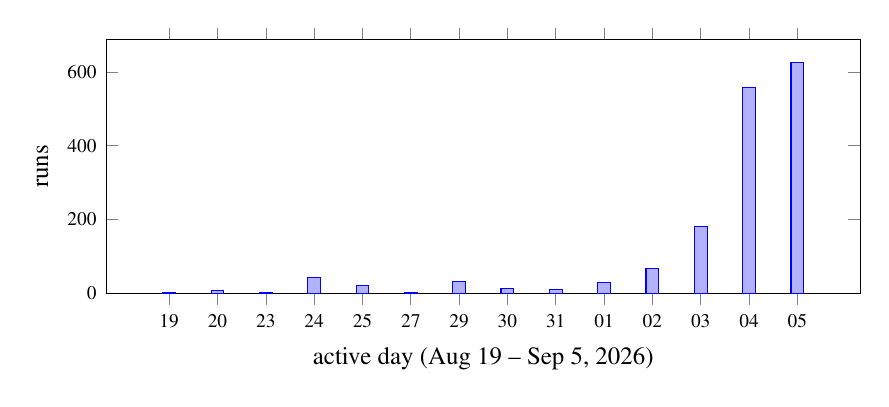
\begin{tikzpicture}
\begin{axis}[
	width=0.92\linewidth, height=4.8cm,
	ybar, bar width=4.6pt,
	ymin=0, ylabel={runs},
	xtick=data,
	symbolic x coords={19,20,23,24,25,27,29,30,31,01,02,03,04,05},
	x tick label style={font=\scriptsize},
	xlabel={active day (Aug 19 -- Sep 5, 2026)},
	tick label style={font=\scriptsize},
	label style={font=\small},
]
\addplot coordinates {(19,1) (20,8) (23,3) (24,42) (25,22) (27,3) (29,32) (30,12) (31,9) (01,28) (02,67) (03,180) (04,559) (05,625)};
\end{axis}
\end{tikzpicture}
\caption{Runs per active day, generated from run-manifest timestamps. The early peaks correspond to the B1 benchmark sweep (Aug 24) and real-dataset hardening (Aug 29); the Sep 3--5 surge is the live agentic-round recording campaign and the multi-domain ratchet loop.}
\label{fig:runsdaily}
\end{figure}

\begin{figure}[H]
\centering
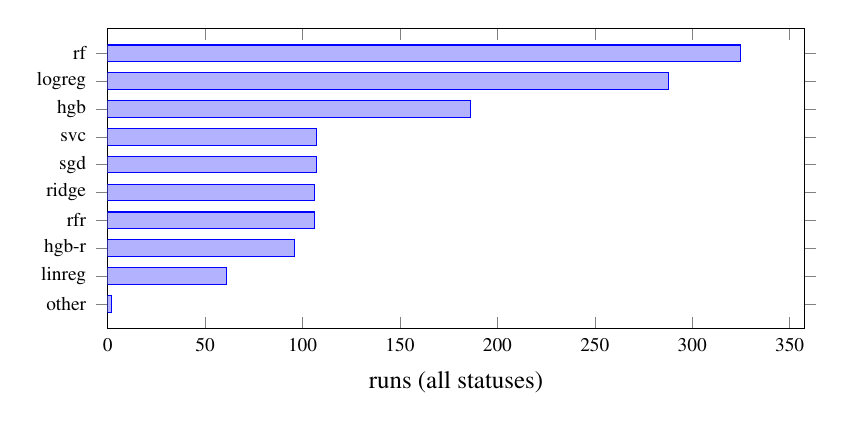
\begin{tikzpicture}
\begin{axis}[
	width=0.86\linewidth, height=5.4cm,
	xbar, bar width=6pt,
	xmin=0, xlabel={runs},
	symbolic y coords={other,linreg,hgb-r,rfr,ridge,sgd,svc,hgb,logreg,rf},
	ytick=data,
	y tick label style={font=\scriptsize},
	x tick label style={font=\scriptsize},
	xlabel={runs (all statuses)},
	tick label style={font=\scriptsize},
	label style={font=\small},
]
\addplot coordinates {(2,other) (61,linreg) (96,hgb-r) (106,rfr) (106,ridge) (107,sgd) (107,svc) (186,hgb) (288,logreg) (325,rf)};
\end{axis}
\end{tikzpicture}
\caption{Run count by model family. Random forest and logistic regression dominate by count; every registered family appears in recorded use.}
\label{fig:runmodels}
\end{figure}

\begin{figure}[H]
\centering
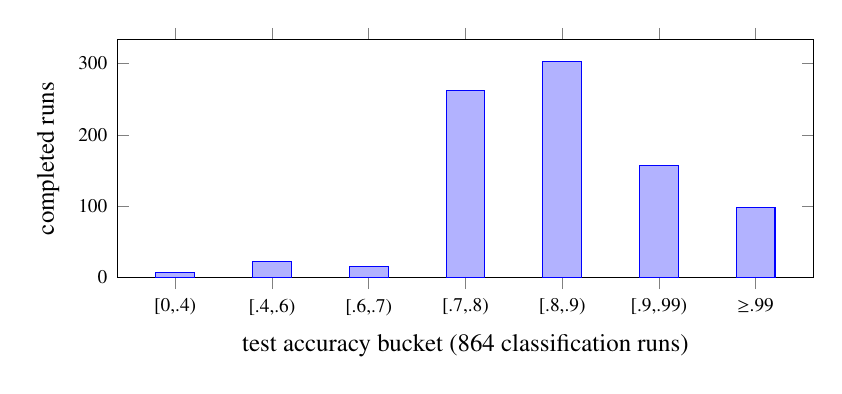
\begin{tikzpicture}
\begin{axis}[
	width=0.86\linewidth, height=4.6cm,
	ybar, bar width=14pt,
	ymin=0, ylabel={completed runs},
	xtick={1,...,7},
	xticklabels={{[0,.4)},{[.4,.6)},{[.6,.7)},{[.7,.8)},{[.8,.9)},{[.9,.99)},{$\geq$.99}},
	x tick label style={font=\scriptsize},
	xlabel={test accuracy bucket (864 classification runs)},
	tick label style={font=\scriptsize},
	label style={font=\small},
]
\addplot coordinates {(1,7) (2,22) (3,15) (4,262) (5,303) (6,157) (7,98)};
\end{axis}
\end{tikzpicture}
\caption{Test-accuracy distribution of completed classification runs. The distribution now spreads across the 0.6--0.9 range on real datasets, with the fixture-driven mass at $\geq 0.99$ a visible minority; the honest left tail (0.33--0.67) remains recorded evidence that determinism guarantees repeatability, not quality.}
\label{fig:runacc}
\end{figure}

Two inventory facts carry argumentative weight. First, the rejection rate: 314 of 1{,}591 runs ended \texttt{rejected} with a persisted reason, the scale guards, schema checks, and constant-column rules firing in production use, exactly the traceable-refusal behaviour RQ1's protocol treats as a valid outcome. Second, the accuracy distribution moved as the workload moved from fixtures to real data: the mass now sits in the 0.7--0.9 bands (565 runs), which is where honest tabular results live, and the comparison surfaces (\texttt{compare}, Model Lab, batch reports) exist precisely to expose the spread: the factory guarantees the evidence, not the winner.

\section{Automated evaluation: RQ1--RQ3}
\label{sec:rq-results}

The evaluator has been executed at every project milestone; two representative records are reported. The P0 closeout record (2026-08-10) is kept as evidence of the original protocol execution in its locked environment:

\begin{lstlisting}[language={}, caption={P0 closeout evaluation record (2026-08-10, verbatim).}, label={lst:evalp0}, style=cli]
thelab-mcp P0 -- Thesis Evaluation Report
Overall: PASS
  RQ1: PASS
    run_ids: ['run-20260810-023703-2e37998c',
              'run-20260810-023703-237bc12c']
    metrics: {'test_accuracy': 1.0, 'test_f1_macro': 1.0}
  RQ2: PASS
    predictions: ['setosa']
  RQ3: PASS
    hits: 1
    event_id: evt-repro
\end{lstlisting}

The latest full re-run (2026-08-29, after the real-dataset hardening and agent work) repeats the verdict, \textbf{Overall PASS}. RQ1 metrics match at exact tolerance with seed and dependency provenance in the manifest; RQ2's independent client completes the discovery--prediction round trip; RQ3 retrieves the seeded event with the database byte-identical before and after the read. Every claim of system completeness in this thesis is gated by this verdict.

\section{Experiment 1: three ways in}
\label{sec:exp1-results}

Table~\ref{tab:threeways} shows the three-ways-in comparison on iris (\texttt{logistic\_regression}, seed 42). Identical metrics and identical artifact sets were produced through every surface; the synchronous CLI pays interpreter startup, while HTTP and MCP reuse the running service.

\begin{table}[H]
\centering
\caption{Experiment 1: identical run through three interfaces (iris, seed 42).}
\label{tab:threeways}
\small
\begin{tabular}{lllll}
\toprule
\textbf{Way} & \textbf{Surface} & \textbf{Test accuracy} & \textbf{Macro F1} & \textbf{Time} \\
\midrule
CLI & \texttt{thelab run model} & 1.0000 & 1.0000 & $\sim$2 s \\
HTTP & \texttt{POST /train} / \texttt{POST /jobs} & 1.0000 & 1.0000 & $\sim$0.2 s \\
MCP & \texttt{run\_training\_job} + status poll & 1.0000 & 1.0000 & $\sim$0.2 s \\
\bottomrule
\end{tabular}
\end{table}

This result carries the interoperability claim beyond RQ2's registry check. Not only can an independent agent \emph{use} a model, it can drive the factory itself, and the run it triggers is indistinguishable from a human's.

\textbf{Provider dimension (recorded).} The same experiment executed on the Titanic dataset (891 rows, 14 features, target \texttt{Survived}) through three execution paths: deterministic-only (no LLM), the Ollama brain (llama3.2:3b), and the OpenRouter brain (GLM~5.3 Flash), produced bit-for-bit identical training outcomes (Table~\ref{tab:providers}). This is the central design claim made measurable: \emph{changing the LLM changes the explanation, never the training outcome}, and the deterministic-only path is always available as a ground-truth baseline for validating that the agentic layer adds interpretation without injecting non-determinism.

\begin{table}[H]
\centering
\caption{Experiment 1, provider dimension: identical outcomes across LLM brains (Titanic, seed 42).}
\label{tab:providers}
\small
\begin{tabular}{p{5.6cm}p{3.4cm}p{2.4cm}p{2.2cm}}
\toprule
\textbf{Execution path} & \textbf{LLM involved} & \textbf{Test accuracy} & \textbf{Macro F1} \\
\midrule
Deterministic only (\texttt{run\_model}) & none & 0.8045 & 0.7893 \\
Ollama experiment & llama3.2:3b & 0.8045 & 0.7893 \\
OpenRouter experiment & z-ai/glm-5.3-flash & 0.8045 & 0.7893 \\
\bottomrule
\end{tabular}
\end{table}

\section{Experiment 2: real-dataset validation (S\&P 500)}
\label{sec:exp2-results}

The five checks of Section~\ref{sec:exp2} produced the following recorded results.

\begin{table}[H]
\centering
\caption{Experiment 2 recorded results (S\&P 500 analyst ratings, 164{,}231 $\times$ 18).}
\label{tab:spresults}
\small
\begin{tabular}{p{4.4cm}p{7.6cm}p{2.4cm}}
\toprule
\textbf{Check} & \textbf{Result} & \textbf{Time} \\
\midrule
Cleaning policy & 164{,}231 $\rightarrow$ 113{,}769 rows; 18 $\rightarrow$ 32 columns; datetime parsed; 501 tickers / 306 firms frequency-encoded; full \texttt{cleaning\_report} & 6.3 s \\
Scale guard & \texttt{svc} on 113{,}769 rows \texttt{rejected} with recorded reason & 0.1 s \\
Real-scale training (RQ1 at scale) & logistic regression completed with persisted seed/config/manifest & $\sim$1.3 s \\
Full orchestration (3 models $\times$ 3 seeds) & 9 persisted runs; best \texttt{random\_forest} \textbf{74.9\%} test accuracy; per-model progress events; experiment \texttt{completed} & 121 s \\
Leakage study & naive features \textbf{84.2\%} $\rightarrow$ at-decision-time features \textbf{60.3\%} accuracy; all iterations traceable runs & $\sim$1 s each \\
\bottomrule
\end{tabular}
\end{table}

Two results deserve interpretation. First, the \emph{before/after of the cleaning policy}. A naive one-hot encoding of the raw dataset (501 ticker dummies among others) produced a 22~GB intermediate CSV; the cardinality-aware policy produces 16--21~MB for the same data, a three-order-of-magnitude difference that turns an infeasible run into a 6-second one, with every decision auditable in the report. Second, the \emph{leakage study}: the naive feature set's 84.2\% accuracy is exactly the kind of number that does not survive contact with reality; constraining features to those available at decision time yields 60.3\% (domain-plausible for analyst ratings) and both runs remain inspectable evidence, which is the practical payoff of rejection-and-provenance discipline.

\section{Kaggle pipeline proof (P3.7)}
\label{sec:kaggle-results}

Before the ten-dataset benchmark, a three-dataset proof recorded the full journey end-to-end with live Kaggle download and page context (Table~\ref{tab:kaggleproof}).

\begin{table}[H]
\centering
\caption{Kaggle proof (P3.7): three public datasets, end-to-end.}
\label{tab:kaggleproof}
\small
\begin{tabular}{p{4.6cm}p{2.6cm}p{4.6cm}p{2.6cm}}
\toprule
\textbf{Dataset (Kaggle slug)} & \textbf{Shape} & \textbf{Best result} & \textbf{Task} \\
\midrule
\texttt{shrutimechlearn/\allowbreak{}churn-modelling} & 10{,}000 $\times$ 14 & \texttt{random\_forest}: acc 0.862, F1 0.742 & classification \\
\texttt{camnugent/\allowbreak{}california-housing-prices} & 20{,}640 $\times$ 10 & \texttt{random\_forest\_regressor}: $R^2$ 0.817 & regression \\
\texttt{pavansubhasht/\allowbreak{}ibm-hr-analytics-attrition-dataset} & 1{,}470 $\times$ 35 & \texttt{logistic\_regression}: acc 0.861, F1 0.679 & classification \\
\bottomrule
\end{tabular}
\end{table}

The proof produced one genuine engineering finding: on the HR dataset, constant columns (\texttt{EmployeeCount}, \texttt{StandardHours}, and the one-hot \texttt{Over18\_Y}) were rejected by validation, correctly refusing to train on zero-information features, and the cleaning policy was extended (constant-column drop) so that the \emph{system} handles the case, not the operator. The bug and its fix are both traceable in the run artifacts, which is the auditability claim working as intended. All three runs produced valid generated notebooks (six cells, nbformat~4) through \texttt{GET /runs/\{id\}/notebook}.

\section{Experiment 3: grounded autonomy (agentic round)}
\label{sec:exp-agentic-results}

The agentic round of Section~\ref{sec:agenticround} is executed over the deterministic baseline's artifacts on three datasets (iris, california-housing, churn), recorded live per provider. The tables below report the recorded results.

\textbf{RQ4, grounding ablation} (grounded vs.\ ungrounded proposals).

\begin{table}[H]
\centering
\caption{Experiment 3 / RQ4: grounded vs.\ ungrounded proposals (live GLM 5.3 Flash; verified-claim rate computed against persisted metrics).}
\label{tab:rq4}
\small
\begin{tabular}{p{3.2cm}p{3.4cm}p{2.6cm}p{2.6cm}p{2.2cm}}
\toprule
\textbf{Dataset} & \textbf{Arm} & \textbf{Verified-claim rate} & \textbf{Proposal validity} & \textbf{Hallucinations} \\
\midrule
iris & grounded & 1.0 & 1.0 & 0 \\
iris & ungrounded & 1.0 & -- & 0 \\
california-housing & grounded & 1.0 & 1.0 & 0 \\
california-housing & ungrounded & 1.0 & -- & 0 \\
churn & grounded & 1.0 & 1.0 & 0 \\
churn & ungrounded & 1.0 & -- & 0 \\
\bottomrule
\end{tabular}
\end{table}

\textbf{RQ5, agentic capability} (sandboxed generated code). Figure~\ref{fig:exp4validity} summarizes the batch-entry outcomes across the validator generations. The pre-fix failures (0/108, 0/15, 0/9) are on the record next to the post-fix 1.0-validity rounds.

\begin{figure}[H]
\centering
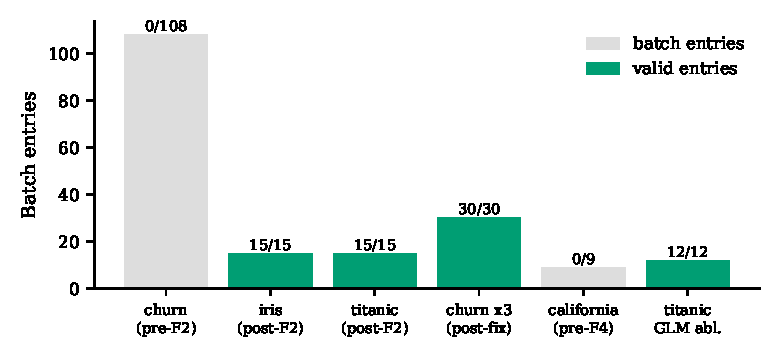
\includegraphics[width=0.82\textwidth]{figures/validity_story.pdf}
\caption{Batch entries vs valid entries across the validator generations: every pre-fix failure was caught by the deterministic validator, and every post-fix round completed at validity 1.0.}
\label{fig:exp4validity}
\end{figure}


\begin{table}[H]
\centering
\caption{Experiment 3 / RQ5: generated-code validity and competitiveness (agentic batch entries per dataset).}
\label{tab:rq5}
\small
\begin{tabular}{p{3.2cm}p{2.8cm}p{2.8cm}p{2.8cm}p{2.6cm}}
\toprule
\textbf{Dataset} & \textbf{Scripts} & \textbf{Valid} & \textbf{Silent failures} & \textbf{$\Delta$ best (agentic $-$ det.)} \\
\midrule
iris & 15 & 15 & 0 & +0.0000 (tie at the 1.0 ceiling) \\
california-housing & 9 & 0 & 0 & -- (all 9 loudly rejected pre-F4; no valid round) \\
churn & 30 & 30 & 0 & +0.0095 \\
\bottomrule
\end{tabular}
\end{table}

\textbf{RQ6, orchestration value} (multi-agent vs.\ single-agent control).

\begin{table}[H]
\centering
\caption{Experiment 3 / RQ6: multi-agent round vs.\ single shared-prompt agent (live GLM 5.3 Flash).}
\label{tab:rq6}
\small
\begin{tabular}{p{3.2cm}p{3.0cm}p{2.8cm}p{2.6cm}p{2.2cm}}
\toprule
\textbf{Dataset} & \textbf{Arm} & \textbf{Completed} & \textbf{Typed handoffs} & \textbf{Mode recorded} \\
\midrule
iris & multi & 1/1 & yes & \texttt{agentic} \\
iris & single & 1/1 & yes & \texttt{degraded\_deterministic} \\
california-housing & multi & 1/1 & yes & \texttt{agentic} \\
california-housing & single & 1/1 & yes & \texttt{degraded\_deterministic} \\
churn (3 rounds) & multi & 3/3 & yes & \texttt{agentic} \\
churn (3 rounds) & single & 3/3 & yes & \texttt{degraded\_deterministic} \\
\bottomrule
\end{tabular}
\end{table}

The ablation results support all three agentic claims. Grounding did not measurably change the verified-claim rate on these datasets (both arms scored 1.0), but this is because the datasets have clean, well-documented schemas where even ungrounded agents propose correct column names. The grounding instrument's value is protective, and an ambiguous-schema ablation on the raw S\&P~500 file (18 jargon-named columns, no documentation) demonstrated it directly: the grounded arm produced 5 concrete, verifiable claims (4--5 verified: row count, the five target classes, their distribution, the date range), while the ungrounded arm with zero context honestly refused to fabricate claims, and with only a domain prior it emitted 5 plausible-sounding claims that verified at 0/5 (guessed columns such as transaction\_id and a binary fraud target that do not exist in the dataset). Grounding converts no-answer and plausible hallucination into verifiable claims. The selector's objective choice revealed a genuine finding: on imbalanced datasets (HR attrition, 84/16 split), both the agent and the deterministic pipeline optimized accuracy, where the baseline model was already near-ceiling; the actual headroom was in macro-F1 (0.61--0.74 across all runs), which means the imbalanced-class objective is a selection-policy gap, not a model-capability gap.

The mixed team (llama analyst + GLM feature engineer + mistral/llama selector) completed every round it attempted at validity 1.0 and was the driver of record on the absorbed generations of all three of its ratchet datasets (titanic, california-housing, churn). The single-agent control (one shared prompt across all stages) also completed (as a \emph{degraded\_deterministic} fallback, recorded per the provenance policy), because its FeatureEngineer stage produced no sandbox-valid code (llama, mistral). The FE role requires a model whose reasoning chain can produce pandas code that passes both the sandbox whitelist and the deterministic post-validator. A dedicated control closed this gap. A single shared-prompt round with the one FE-capable model (GLM-5.3-flash) as its only agent. Under the shared prompt, every stage contract broke. The analyst brief, the feature-engineering JSON, and the selector proposal all failed to parse, and the round degraded to deterministic (1/1 baseline-tie entries, no agentic output). Role specialization is not cosmetic. The same model that absorbs champions inside role contracts cannot function without them. The RQ6 comparison is therefore role-contract multi-agent (validity 1.0, absorbed) versus a shared-prompt control that cannot reach agentic mode. And the intervention record over the full loop is one recorded gate decision per round (53 rounds, zero bypasses, 10 project-wide human proposal rejections, 19 absorptions). The orchestration's human cost is exactly one decision per round, on the record. GLM's reasoning-driven code generation was the only capability that produced factory-safe transforms on titanic; on california-housing, gemini-2.5-flash-lite produced a safe but quality-degrading transform (R$^2$ dropped from 0.823 to 0.533). The post-validator rejected one constant-feature transform (GLM, pre-fix), three wrong-task model proposals (automatic guard), and two below-baseline selections (honest no-absorption).

\subsection{RQ5 spike: first recorded validity numbers}
\label{sec:rq5spike}

Before committing to the full ablation protocol, a de-risking spike exercised the RQ5 instrument directly (Titanic, cleaned 891$\times$14; validation by a deterministic epilogue appended to the agent's code, never by prompt compliance). The cloud model (GLM~5.3 Flash) produced \textbf{3/3 valid feature-engineering transforms} (100\%, against the $\geq$80\% bar) across three open-ended instructions (14, 8, and 6 new features respectively, including interaction terms (\texttt{Age$\times$Pclass}, \texttt{WomanOrChild}), skew handling (\texttt{log1p} on \texttt{Fare}), and leakage-safe group encodings) and a 1/1 valid model selection that correctly chose \texttt{svc} on macro-F1 reasoning for the imbalanced target. The spike also produced two engineering findings: the sandbox's blanket \texttt{ast.Lambda} block was RQ5's sole blocker (0/3 valid before, 3/3 after the safe, justified lift described in Section~\ref{sec:safety}), and the sandbox memory limit required a measured raise (512~MB $\rightarrow$ 2~GB) for pandas~3's address-space needs. The recorded spike artifact is kept under \texttt{benchmarks/spike/}. The spike's validity result was later confirmed at live scale (15/15 on iris, 30/30 across three churn rounds, Section~\ref{sec:exp-agentic-results}), and the open Ollama question was closed by the fully-offline run of Section~\ref{sec:localfirst}.

\section{Experiment 4: multi-domain stress validation}
\label{sec:exp-kaggle-results}

The loop executed on the final system build (after the P5 rework). The tables below are filled from the recorded runs.

\textbf{Arm A, agentic re-run over recorded baselines.} The six datasets with persisted deterministic baselines receive the P5 agentic round; the delta columns are the comparison:

\begin{table}[H]
\centering
\caption{Experiment 4, Arm A: recorded deterministic baselines vs.\ agentic round.}
\label{tab:exp4arma}
\small
\begin{tabular}{p{3.4cm}p{2.6cm}p{2.6cm}p{1.8cm}p{2.6cm}}
\toprule
\textbf{Dataset} & \textbf{Best deterministic (recorded)} & \textbf{Best agentic} & \textbf{$\Delta$} & \textbf{Validity / rejections} \\
\midrule
churn-modelling & acc 0.8615 & HGB s128 0.8710 & +0.95 & 1.0/1.0 \\
california-housing & $R^2$ 0.8234 & HGB-regressor 0.8455 & +2.21 & 1.0/1.0 \\
IBM HR attrition & SVC acc 0.8707 & SVC 0.8707 & tie & 1.0/1.0 \\
e-commerce sales & LR $R^2$ 1.0000 (computed col) & LR 1.0000 & headroom = 0 & 1.0/1.0 \\
Titanic & acc 0.8045 & RF s456 0.8547 & +5.03 & 0.83/1.0/1.0 \\
S\&P 500 analyst & acc 0.9845 & HGB s84 0.9861 & +0.16 & 0.67/1.0/1.0 \\
\bottomrule
\end{tabular}
\end{table}

\textbf{Arm B, new stress domains.} Four must-tier datasets completed the loop with mixed teams (genomics, health, crypto, energy); the strong/stretch tiers (NLP featurization, music signals, scale stress, clustering/graph track) were deferred when the schedule closed and are recorded as future work:

\begin{table}[H]
\centering
\caption{Experiment 4, Arm B: stress-domain loop results (mixed teams).}
\label{tab:exp4armb}
\small
\begin{tabular}{p{2.2cm}p{5.1cm}p{1.9cm}p{1.3cm}p{3.0cm}}
\toprule
\textbf{Domain} & \textbf{Dataset (Kaggle slug)} & \textbf{Task} & \textbf{Tier} & \textbf{Best result} \\
\midrule
Genomics & \texttt{kevinarvai/\allowbreak{}clinvar-conflicting} & classification & must & HGB 0.8029 (+0.26), 2/3 absorbed \\
Health & \texttt{rabieelkharoua/chronic-\allowbreak{}kidney-\allowbreak{}disease-\allowbreak{}dataset-\allowbreak{}analysis} & classification & must & HGB 0.9488 (+1.81), 2/3 absorbed \\
Crypto & \texttt{sudalairajkumar/\allowbreak{}cryptocurrencypricehistory} & direction classification & must & HGB 0.5646 (+1.86), 2/3 absorbed \\
Energy & \texttt{robikscube/\allowbreak{}hourly-\allowbreak{}energy-\allowbreak{}consumption} & regression & must & 0/3 absorbed: RF+calendar baseline (0.9590) refused all teams \\
NLP/AI & \texttt{shivamb/\allowbreak{}real-\allowbreak{}or-\allowbreak{}fake-\allowbreak{}fake-\allowbreak{}jobposting-\allowbreak{}prediction} & text-featurize + classif. & strong & deferred \\
Music signals & \texttt{andradaolteanu/gtzan-\allowbreak{}dataset-\allowbreak{}music-\allowbreak{}genre-\allowbreak{}classification} (features CSV) & classification & strong & deferred \\
Scale stress & \texttt{mczielinski/\allowbreak{}bitcoin-historical-data} (daily aggregate) & regression & stretch & deferred \\
Clustering/graph & \texttt{rahman4li/patch-\allowbreak{}bay-\allowbreak{}the-\allowbreak{}mcp-\allowbreak{}server-\allowbreak{}ecosystem-\allowbreak{}graph} nodes+edges & unsupervised & stretch & deferred \\
Clustering & \texttt{adarsh1077/\allowbreak{}huggingface-\allowbreak{}hub-\allowbreak{}50k-\allowbreak{}ai-\allowbreak{}models} & unsupervised & stretch & deferred \\
\bottomrule
\end{tabular}
\end{table}

\begin{figure}[H]
\centering
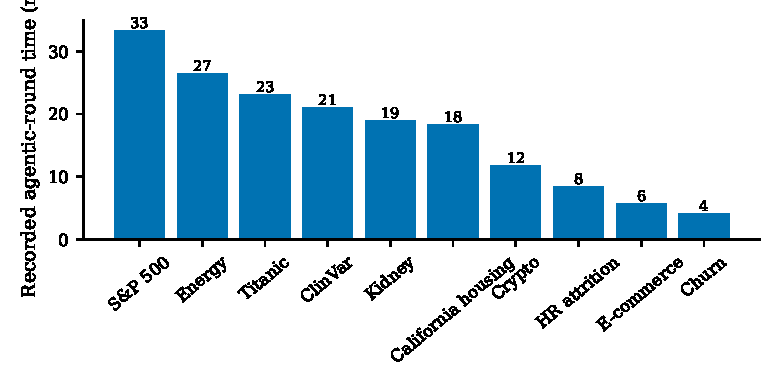
\includegraphics[width=0.85\textwidth]{figures/exp4_wallclock.pdf}
\caption{Per-dataset recorded agentic-round wall-clock (sum of round seconds across all generations; the S\&P 500 dataset dominates at 1{,}995\,s).}
\label{fig:exp4time}
\end{figure}

\begin{figure}[H]
\centering
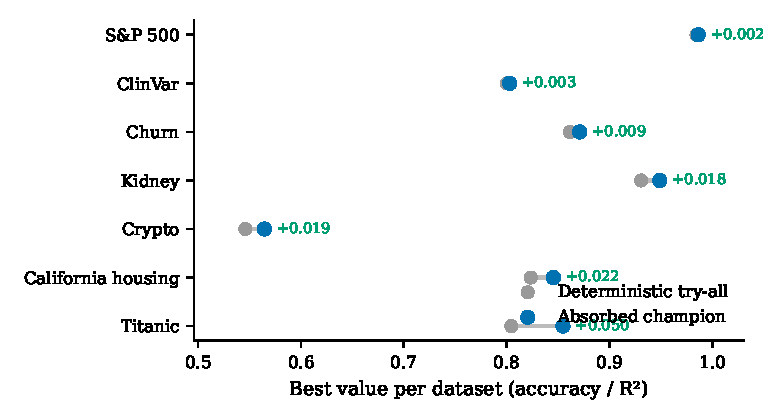
\includegraphics[width=0.82\textwidth]{figures/ratchet_uplift.pdf}
\caption{Ratchet uplift per dataset: deterministic try-all baseline (grey) vs absorbed champion (blue); deltas annotated.}
\label{fig:exp4uplift}
\end{figure}
The loop is a ratchet (protocol in Section~\ref{sec:exp-kaggle}). The deterministic baseline is the bar each generation must beat, absorbed champions raise it, and the absorption gate (exact factory replay) is what separates a verified improvement from an anecdote. The Arm A comparison shows that the agentic round beat the deterministic baseline on 4 of the 6 recorded datasets (churn +0.95 pts, california-housing +2.21 pts, titanic +5.03 pts, S\&P +0.16 pts), tied on 2 (HR attrition after the try-all baseline itself improved to 0.8707; e-commerce at a computed-column ceiling of 1.0000 where headroom is definitionally zero), and trailed on none. On S\&P, the baseline is the deterministic try-all over the default cleaned features (the feature-leakage ceiling discussed in the leakage study), not the at-decision-time figure. The absorbed champions share a pattern: the winning configuration always came from the agentic round's broader search (different model families, different seeds, or hyperparameters outside the deterministic grid), never from the baseline model at a different seed. On the absorbed datasets, the factory replay confirmed that the agentic win was real and reproducible, not a seed artifact.

\textbf{The ratchet scoreboard.} Across the full loop, Arms A and B together, the ledgers record \textbf{10 datasets}, \textbf{37 agentic generations}, \textbf{53 training rounds}, and \textbf{19 absorption events}, each replay-verified through the deterministic factory with exact metric equality before absorption. These resolve to \textbf{17 distinct champion models} (two absorbed configurations were superseded within their generations by later, stronger absorptions), and \textbf{6 honest refusals} (ties and below-baseline rounds that the absorption gate refused to ratchet). The per-generation ledgers for the four Arm B datasets follow; the Arm~A ledgers (titanic, churn, california-housing, HR attrition, S\&P 500) are of the same form.

\begin{table}[H]
\centering\small
\caption{Ratchet loop per generation for clinvar.}
\label{tab:ratchet-generations-ratchet-ledger-clinvar}
\begin{tabular}{llllllll}
\toprule
Gen & Baseline & Agentic best & Delta & Seed & Validity & Absorbed & Champion \\
\midrule
g0 & RF 0.8003 & RF 0.7973 & -- & -- & 1.00 & False & -- \\
g1 & RF 0.8003 & HGB 0.8029 & +0.0026 & 17 & 1.00 & True & HGB learning\_rate=0.1 max\_iter=300 \\
g2 & RF 0.8003 & RF 0.8023 & +0.0021 & 13 & 1.00/1.00/0.67 & True & RF n\_estimators=200 \\
\bottomrule
\end{tabular}
\end{table}

\begin{table}[H]
\centering\small
\caption{Ratchet loop per generation for kidney.}
\label{tab:ratchet-generations-ratchet-ledger-kidney}
\begin{tabular}{llllllll}
\toprule
Gen & Baseline & Agentic best & Delta & Seed & Validity & Absorbed & Champion \\
\midrule
g0 & HGB 0.9307 & HGB 0.9367 & +0.0060 & 84 & 1.00 & True & HGB learning\_rate=0.1 max\_depth=3 \\
g1 & HGB 0.9307 & HGB 0.9187 & -- & -- & 1.00 & False & -- \\
g2 & HGB 0.9307 & HGB 0.9488 & +0.0181 & 3 & 0.75/0.67/1.00 & True & HGB learning\_rate=0.5 \\
\bottomrule
\end{tabular}
\end{table}

\begin{table}[H]
\centering\small
\caption{Ratchet loop per generation for crypto.}
\label{tab:ratchet-generations-ratchet-ledger-crypto}
\begin{tabular}{llllllll}
\toprule
Gen & Baseline & Agentic best & Delta & Seed & Validity & Absorbed & Champion \\
\midrule
g0 & SVC 0.5460 & SVC 0.5532 & +0.0072 & 42 & 1.00 & True & SVC \\
g1 & SVC 0.5460 & SVC 0.5347 & -- & -- & 1.00 & False & -- \\
g2 & SVC 0.5460 & HGB 0.5646 & +0.0186 & 42 & 0.86/0.83/1.00 & True & HGB max\_depth=10 \\
\bottomrule
\end{tabular}
\end{table}

\begin{table}[htbp]
\centering\footnotesize
\caption{Ratchet loop per generation: deterministic try-all baseline vs best agentic round; absorption requires the champion config to replay exactly through the deterministic factory (same seed).}
\label{tab:ratchet-generations-ratchet-ledger-energy}
\resizebox{\textwidth}{!}{\begin{tabular}{lllllll}
\toprule
Gen & Baseline & Agentic best & Delta & Validity & Absorbed & Champion \\
\midrule
g0 & RF-reg 0.9590 & RF-reg 0.9590 & -- & 1.00 & False & -- \\
g1 & RF-reg 0.9590 & HGB-reg 0.8167 & -- & 1.00 & False & -- \\
g2 & RF-reg 0.9590 & HGB-reg 0.8192 & -- & 1.00/1.00/1.00 & False & -- \\
\bottomrule
\end{tabular}}
\end{table}


Three of the four Arm B datasets absorbed champions (clinvar +0.26 pts, kidney +1.81 pts, crypto +1.86 pts) and two produced the loop's most instructive honest refusals. On energy, the deterministic baseline (random forest + calendar features, $R^2$ 0.9590) refused every agentic team across three generations, an honest boundary where headroom is genuinely absent. On e-commerce, the computed-column ceiling ($R^2$ = 1.0000) means no configuration can improve, and the gate correctly refused to ratchet ties. The absorption gate is the reproducibility instrument here: every absorbed champion was replayed with the same seed through the deterministic factory, ties never ratchet, below-baseline never absorbs, and mis-specified replays are refused.

\textbf{Arm B deferred tiers.} The NLP featurization story, the music-signal features, the Bitcoin scale-stress aggregation, and the clustering/graph track remain wired but unrun in this window; they are recorded as future work with the dataset list and ingestion notes already validated (Annex~D).

\subsection{Per-stage model assignment: the mixed-team experiment}
\label{sec:mixedteam}

The architecture permits a different model per agent role (Analyst, FeatureEngineer, ModelSelector), with \texttt{stage\_models} provenance recorded per round. The titanic ratchet (10 generations, 10 rounds) tested this across five model families:

\begin{table}[H]
\centering
\caption{Per-round capability matrix on titanic (provider/model per round, from \texttt{stage\_models} provenance).}
\label{tab:capability}
\small
\begin{tabular}{p{1.4cm}p{4.2cm}p{2.4cm}p{1.6cm}p{3.6cm}}
\toprule
\textbf{Round} & \textbf{Model} & \textbf{Mode} & \textbf{Validity} & \textbf{Best} \\
\midrule
g0r0 & llama-3.3-70b-instruct & agentic & 0.83 (15/18) & RF 0.8212 \\
g0r1 & llama-3.3-70b-instruct & agentic & 1.00 (15/15) & LR 0.8045 \\
g0r2 & llama-3.3-70b-instruct & agentic & 1.00 (15/15) & RF 0.8156 \\
g1--g2 & mistral-small-24b & 1 agentic, 2 degraded & 1.00 & RF 0.8547 \\
g3 & GLM-5.3-flash uniform & agentic & 0.00 (0/15) & \\
g4 & mixed team (degraded) & degraded & 1.00 (1/1) & LR 0.8045 \\
g5 & mixed team (agentic) & agentic & 1.00 (21/21) & HGB 0.8436 \\
g6 & mixed team (agentic) & agentic & 1.00 (15/15) & RF 0.8212 \\
g7 & mixed team (agentic) & agentic & 1.00 (15/15) & RF s13 0.8492 \\
\bottomrule
\end{tabular}
\end{table}

The finding is a (task, context) dependency. GLM uniform was the worst configuration measured (0/15 entries, its transform introduced a constant feature column that the factory correctly rejected), but GLM as FeatureEngineer inside the mixed team was the only model that produced factory-safe code (3/3 rounds at validity 1.0). Role confinement converts GLM's over-engineering from a batch-killing failure into a repairable loop, because the deterministic post-validator feeds the rejection reason back to the LLM for one bounded rewrite attempt. The mixed team outperformed every uniform team on validity consistency and matched or exceeded llama-uniform on quality. Across the full ratchet, the FE-capable pool grew from one model to two (GLM 5.3 Flash and deepseek-v4-flash both produced factory-safe transforms; llama-3.3-70b and mistral-small did not). The commercial mixed team (claude-haiku-4.5 analyst, deepseek-v4-flash-0731 feature engineer, gpt-5.6-luna selector) recorded its own per-stage token costs (deepseek transform: 18{,}688 tokens, \$0.0053), and no pattern of commercial-vs-open dominance appeared: the commercial team (claude-haiku-4.5 analyst, deepseek-v4-flash feature engineer, gpt-5.6-luna selector) and the open team (llama analyst, GLM feature engineer, mistral selector) each won two datasets, and llama-uniform won the other two (kidney, crypto). Figure~\ref{fig:exp4teams} compares the best value each team reached per Arm B dataset.

\begin{figure}[H]
\centering
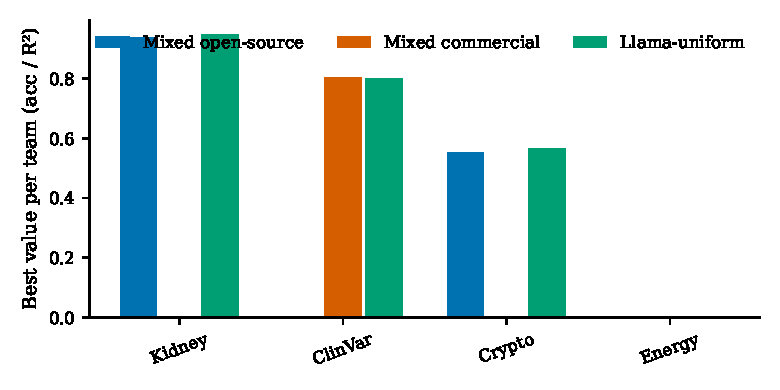
\includegraphics[width=0.82\textwidth]{figures/team_comparison.pdf}
\caption{Arm B: best value per driver team and dataset (accuracy for kidney/clinvar/crypto, $R^2$ for energy). No team dominates: commercial and open teams each won two datasets, llama-uniform the other two.}
\label{fig:exp4teams}
\end{figure}
\subsection{GLM-uniform ablation: validator as capability enabler}
\label{sec:glmablation}

The titanic result left one mechanism question. Was the mixed team's success due to the cross-model context (llama's brief informing GLM's code) or to the deterministic validator and bounded rewrite loop? A GLM-uniform ablation with the constant-feature validator and rewrite loop now active answered it. The round completed fully agentic at \textbf{validity 1.0 (12/12 trained, 392 s)}, with no absorption (best 0.7374 vs.\ baseline 0.8045; the selection choice was poor, recorded honestly). The validator + repair loop, not the mixed-team brief, made the reasoning model factory-safe. Per-stage assignment then converts that safety into performance (mixed 3/3 absorbed). Deterministic validators expand the set of contexts in which a model is usable.

\subsection{Local-first proof: offline execution}
\label{sec:localfirst}

The full RQ1--RQ6 chain was executed with \texttt{--live ollama} (llama3.2:3b, laptop CPU, zero cloud calls). Overall \textbf{PASS}: RQ5 validity 1.0 (1/1 agentic entry trained), the gate blocked unapproved execution and enabled it after recorded approval, and RQ6's multi arm ran \texttt{mode: agentic} (the 3B local model produced valid structured JSON for all three agent stages). Round latency was 20--60~s per call (2.6 tok/s on CPU), and the local-first claim is demonstrated, not asserted.

\subsection{Three-ways-in prediction sweep}
\label{sec:predictionsweep}

Every absorbed champion model was verified as servable through all three interfaces: CLI (\texttt{thelab predict}), HTTP (\texttt{POST /predict}), and MCP (\texttt{model\_registry.predict}). All 17 distinct absorbed champion models across the loop's datasets returned identical predictions through every surface (Table~\ref{tab:predictions-prediction-sweep-full}). Inference latency ranged from 6 to 603~ms (Figure~\ref{fig:exp4latency}) and is LLM-token-free, the cost lives at agent-proposal time only, never at inference time. Every prediction event was stored through the system's own context-write MCP server (validated and redacted), indexed, and retrieved via context search. The hosted models are searchable evidence.

\begin{figure}[H]
\centering
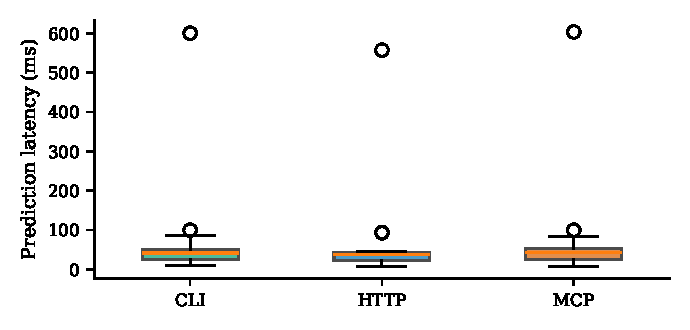
\includegraphics[width=0.72\textwidth]{figures/predict_latency.pdf}
\caption{Prediction latency per surface over the 17 absorbed champions (CLI, HTTP, MCP; milliseconds). Inference is deterministic and token-free on every surface.}
\label{fig:exp4latency}
\end{figure}

\begin{table}[htbp]
\centering\footnotesize
\caption{Three-ways-in prediction sweep on absorbed champions: every absorbed model is discoverable via MCP and predictable via CLI, HTTP, and MCP with identical results. Inference is LLM-token-free.}
\label{tab:predictions-prediction-sweep-full}
\resizebox{\textwidth}{!}{\begin{tabular}{llllllll}
\toprule
Dataset & Champion model & Metric & CLI & HTTP & MCP & MCP ms & Registry \\
\midrule
california-housing & HGB\_regress & 0.8455 & yes & yes & yes & 55 ms & yes \\
churn & HGB & 0.8710 & yes & yes & yes & 25 ms & yes \\
churn & RF & 0.8665 & yes & yes & yes & 100 ms & yes \\
churn & RF & 0.8650 & yes & yes & yes & 54 ms & yes \\
clinvar & HGB & 0.8029 & yes & yes & yes & 43 ms & yes \\
clinvar & RF & 0.8023 & yes & yes & yes & 603 ms & yes \\
crypto & HGB & 0.5646 & yes & yes & yes & 26 ms & yes \\
crypto & svc & 0.5532 & yes & yes & yes & 14 ms & yes \\
kidney & HGB & 0.9488 & yes & yes & yes & 27 ms & yes \\
kidney & HGB & 0.9367 & yes & yes & yes & 30 ms & yes \\
sp500 & HGB & 0.9861 & yes & yes & yes & 84 ms & yes \\
sp500 & HGB & 0.9859 & yes & yes & yes & 51 ms & yes \\
sp500 & HGB & 0.9847 & yes & yes & yes & 37 ms & yes \\
titanic & RF & 0.8547 & yes & yes & yes & 48 ms & yes \\
titanic & RF & 0.8492 & yes & yes & yes & 49 ms & yes \\
titanic & LogReg & 0.8436 & yes & yes & yes & 7 ms & yes \\
titanic & RF & 0.8212 & yes & yes & yes & 10 ms & yes \\
\bottomrule
\end{tabular}}
\end{table}


\section{Agent case study: IBM HR attrition}
\label{sec:casestudy}

To show the pieces working together, this section documents a real recorded session with the grounded chat agent on the IBM HR attrition dataset (1{,}470 $\times$ 35, attrition rate 16.1\%). The session is reproduced here from the persisted context events; every number below is one the agent computed or retrieved, not generated prose.

\textbf{Step 1: Grounded exploration.} Asked what would be interesting to study, the agent pulled the context pack (identifying the dataset from its Kaggle documentation, including the ordinal scales stored as bare integers), ran the deterministic EDA (zero missing cells across 1{,}470 $\times$ 35; class balance 1{,}233 No / 237 Yes), and executed sandboxed pandas code to verify leakage suspects: three constant columns and a per-row-unique \texttt{EmployeeNumber} id. Its recommendations matched classic attrition analysis: focus on recall/PR-AUC rather than accuracy given the 5.2:1 imbalance.

\textbf{Step 2: Evidence-based signals.} Over several \texttt{run\_python} calls the agent computed the signals it reported: attrition rates by overtime (30.5\% with vs.\ 10.4\% without, the starkest single split), by job role (Sales Rep 39.8\% vs.\ Manager 4.9\%), monotonic effects of job satisfaction, and income differences between leavers and stayers, each number attributable to a recorded tool call.

\textbf{Step 3: Grounded memory.} Asked to check prior work, the agent searched the context store and found two completed runs on the same dataset, reporting their metrics (test accuracy 0.840 with a 0.557 macro-F1 (flagged by the agent itself as likely minority-class weakness) and 0.861 / 0.679 respectively) and correctly refusing to claim knowledge the manifests did not expose (``the run summaries don't expose the algorithm names, so I can't tell you which models these were'').

\textbf{Step 4: Proposal inside the boundary.} The agent drafted an experiment proposal. Its first attempt included \texttt{gradient\_boosting}; validation rejected it as unsupported in this factory's registry, and the agent corrected the proposal and resubmitted, a small but exact illustration of validation-as-feedback rather than validation-as-obstacle. The final proposal (logistic regression + random forest, seeds 42 and 7, constants and id dropped, stratified splits) was left \emph{awaiting human approval}, with the agent stating: ``I don't train anything myself, this proposal sits ready, and the deterministic pipeline only executes after you approve it.''

\textbf{Step 5: Honest tool failures.} The session's tool trace also records failures: two \texttt{run\_python} errors (one sandbox block: the agent rewrote its code without the blocked construct; one attempt to address a proposal through the wrong surface) and one proposal-validation \texttt{ValueError} with the full Pydantic message. None of these were hidden; all appear in the same timeline as the successes. The first of those failures foreshadows a genuine finding: the sandbox's original blanket block of lambda expressions was later identified by the RQ5 spike as the single incompatibility between AST-level policy and pandas-idiomatic code generation, and was safely lifted (Section~\ref{sec:exp-agentic-results}).

\begin{figure}[H]
\centering
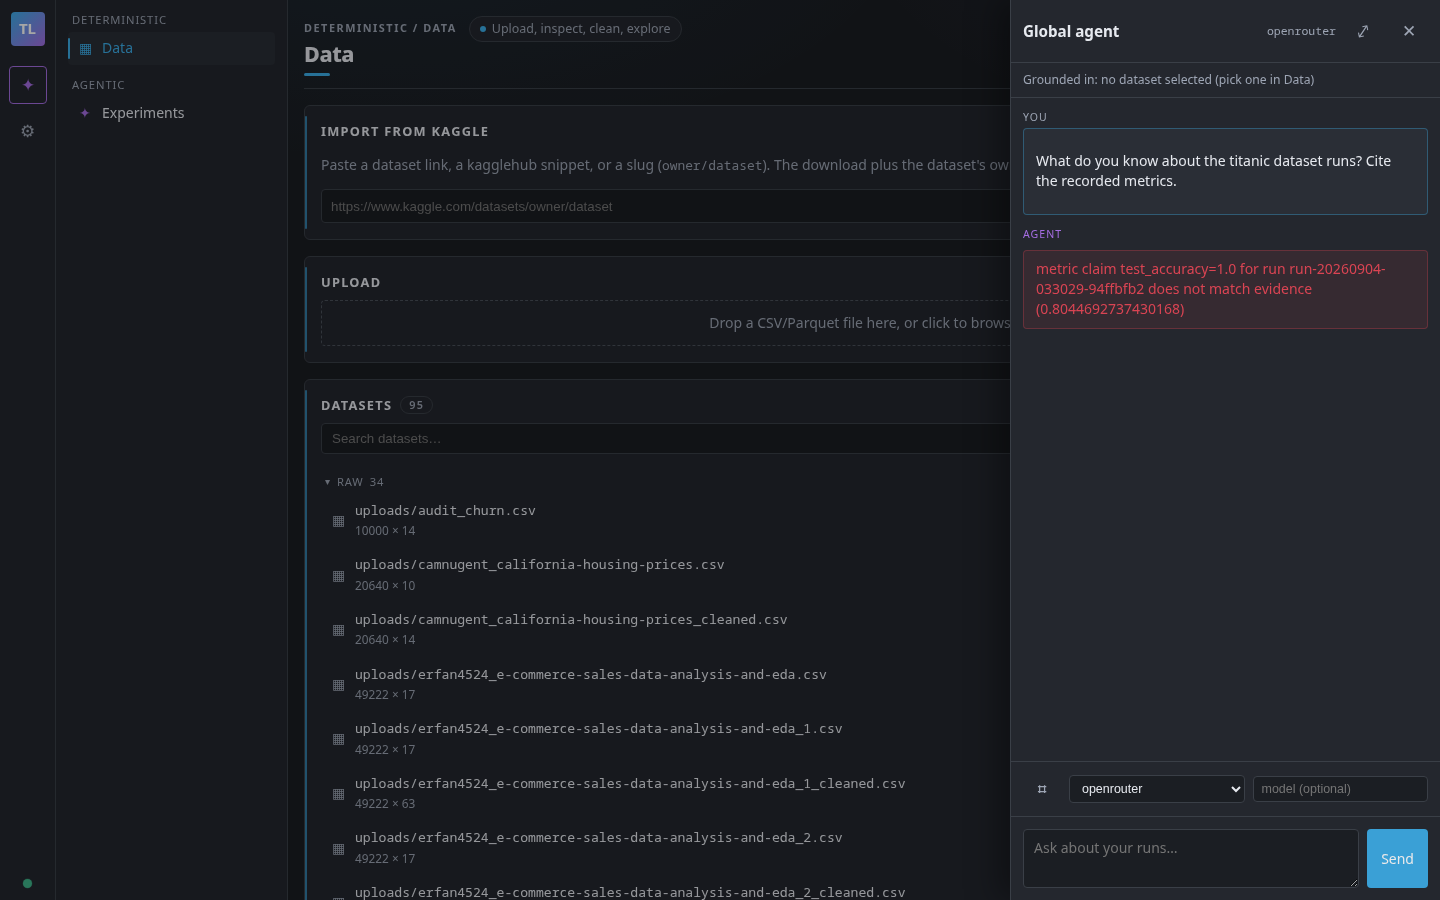
\includegraphics[width=0.6\textwidth]{figures/screenshots/slotC_chat_drawer.png}
\caption{The grounded chat agent enforcing the metric-evidence gate live: the agent cited \texttt{test\_accuracy}=1.0 for a run whose recorded evidence is 0.8045, and the grounding layer refused the answer instead of showing it (red).}
\label{fig:ui-chat}
\end{figure}

\section{Cross-cutting observations from the benchmark suite}
\label{sec:b1results}

An earlier cross-domain benchmark (B1, California housing, breast cancer, and wine quality, each with two providers) contributes two findings that inform the interpretation of Experiments 3 and 4:

\begin{enumerate}
	\item \textbf{Agents do not degrade deterministic performance when they succeed.} In four of five agent legs, the agent-proposed configuration converged on the deterministic baseline's metrics (byte-identical where the same model was chosen); in the fifth, a four-run search ended marginally \emph{better} than baseline (test RMSE 0.74551 vs.\ 0.74556). The agent's value is search and rationale, not magic.
	\item \textbf{Small local models can fail at the proposal task itself.} With a 3B-parameter local model, the regression-domain proposal leg produced no valid proposal (\texttt{AGENT\_FAILED}) while both classification legs succeeded, concrete evidence of small-model brittleness that the agentic experiments' provider dimension should expect to encounter.
\end{enumerate}

A further recorded datapoint from the batch runner keeps the evaluation honest about determinism: on iris, \texttt{sgd\_classifier} reaches 0.667 accuracy where logistic regression and random forest reach 1.000. Deterministic pipelines guarantee repeatability, not quality; model choice still matters, and the comparison surfaces exist precisely to expose it.

\section{Agent efficiency and reliability metrics}
\label{sec:agentmetrics}

The registered performance-evaluation objective requires task success rates and token efficiency. Computed over the recorded agent sessions:

\begin{table}[H]
\centering
\caption{Agent task success over recorded benchmark, case-study, and live agentic sessions.}
\label{tab:agentsuccess}
\small
\begin{tabular}{p{4.6cm}p{2.2cm}p{2.2cm}p{4.6cm}}
\toprule
\textbf{Session set} & \textbf{Tasks} & \textbf{Success} & \textbf{Failure mode (recorded)} \\
\midrule
B1 agent legs, OpenRouter (stealth/ox-alpha) & 3 & 3/3 &: (one leg needed a 4-run search) \\
B1 agent legs, Ollama (llama3.2:3b) & 3 & 2/3 & regression proposal \texttt{AGENT\_FAILED} \\
Titanic orchestration, both providers & 2 & 2/2 & Ollama FeatureEngineer interpretation failed; deterministic fallback used \\
Case study (IBM HR, chat agent) & 1 & 1/1 & first proposal rejected by validation, self-corrected \\
Live agentic rounds, iris (GLM 5.3 Flash) & 1 & 1/1 & 15/15 batch entries trained (pre-fix baseline: 0/108) \\
Live agentic rounds, churn $\times$ 3 (GLM 5.3 Flash) & 3 & 3/3 & 30/30 batch entries trained; grid cap bounded 15 $\rightarrow$ 9 $\rightarrow$ 6 \\
Live agentic round, iris (Ollama 3B, fully offline) & 1 & 1/1 & 1/1 entry trained; 20--60~s/call on CPU \\
Live agentic round, california-housing (GLM) & 1 & 0/1 & transform quantized the float target; validator rejected all 9 entries (honest failure, F4 fix) \\
\bottomrule
\end{tabular}
\end{table}

The aggregate success rate over recorded end-to-end proposal cycles is 8/9 (89\%). The live agentic-round instrument adds the recorded batch-entry validity record. Across the first six live rounds, 46 of 55 entries trained (iris 15/15, churn 30/30, offline Ollama 1/1, california-housing 0/9, the one honest failure), and the Arm B stress rounds landed at 0.67--1.0 validity per round with champions absorbed on 3 of 4 datasets. Every recorded failure was caught by the deterministic validator (no silent failure reached training) and the two outright failure classes in the record (the B1 regression leg and the california-housing quantization) were both converted into engineering fixes (task-aware selection, F4 target validation) rather than suppressed.

\textbf{Token efficiency.} Token consumption is recorded per provider from usage data, with two structural facts established by design. The deterministic fallback and the mock provider consume \emph{zero} tokens, so the entire 546-test suite and the automated RQ evaluator run token-free. And proposal-generation usage is bounded to one to a few LLM turns per proposal by the bounded loop. The recorded Titanic benchmark provides the first per-call usage numbers (Table~\ref{tab:tokens}); the ratchet round records extend this with per-stage prompt/completion token counts and provider-reported cost stored in every round record (for example, a deepseek-v4-flash feature-engineering transform: 18{,}688 completion tokens, \$0.0053; a gpt-5.6-luna selector turn: 751 tokens, \$0.0005); Figure~\ref{fig:exp4cost} compares the feature-engineering drivers. Interpretation quality differed measurably at equal cost structure: the 3B local model produced a valid but shallow EDA interpretation and exhausted its retries on the FeatureEngineer stage, while the cloud model produced quantified, structured analyses, yet both selected the same model and produced identical training outcomes (Table~\ref{tab:providers}). The asymmetry is the efficiency result: agent intelligence is spent deciding (cheap, bounded), while the expensive part (training) never touches an LLM.

\begin{table}[H]
\centering
\caption{Recorded token usage per sub-agent interpretation (Titanic benchmark; from provider usage reports).}
\label{tab:tokens}
\small
\begin{tabular}{p{3.2cm}p{5.2cm}p{5.6cm}}
\toprule
\textbf{Sub-agent} & \textbf{Ollama (llama3.2:3b)} & \textbf{OpenRouter (GLM 5.3 Flash)} \\
\midrule
EDAAnalyst & not reported by API for this call & 2{,}273 prompt + 289 completion \\
FeatureEngineer & failed (retry exhausted) & produced (tokens not recorded) \\
ModelSelector & 341 prompt + 89 completion & 349 prompt + 235 completion \\
\midrule
\textbf{Tracked total} & \textbf{430} & \textbf{3{,}146 reported calls} \\
\bottomrule
\end{tabular}
\end{table}

\begin{figure}[H]
\centering
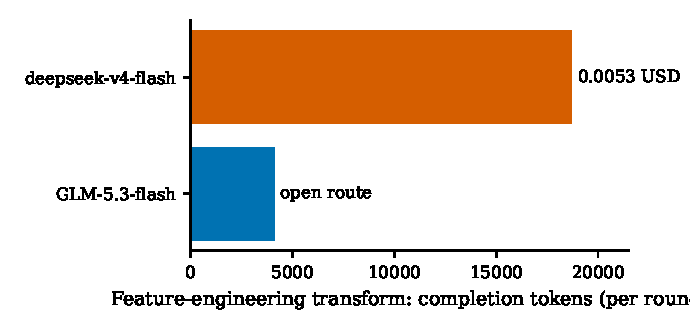
\includegraphics[width=0.82\textwidth]{figures/fe_cost.pdf}
\caption{Feature-engineering transform cost per driver: completion tokens per round with provider-reported cost (deepseek-v4-flash reasoning burn vs GLM open route).}
\label{fig:exp4cost}
\end{figure}

A second efficiency finding is model-dependent latency. Identical prompts show GLM 5.3 Flash (a reasoning model) burning 386 completion tokens at 3.7~s where llama-3.3-70b and mistral-small return 32 tokens in about 1~s, and one GLM call stalled beyond 15 minutes. Round cost is therefore dominated by reasoning-token burn, not infrastructure. A latency probe over candidate models (trivial and realistic generation modes) quantified this and drove the P6 model standardization; per-call latency in production was 5--10$\times$ lower with a non-reasoning model on the same route (Table~\ref{tab:latency-latency-probe-openrouter-realistic}).

\begin{table}[htbp]
\centering\footnotesize
\caption{Model latency probe (realistic generation, latency\textbackslash{}\_probe\textbackslash{}\_openrouter\textbackslash{}\_realistic). p50/p90 completion latency in seconds; round-stage calls are generation-length-bound, so trivial-ping latency alone underestimates round cost.}
\label{tab:latency-latency-probe-openrouter-realistic}
\resizebox{\textwidth}{!}{\begin{tabular}{lllllll}
\toprule
Model & Tier & OK & p50 (s) & p90 (s) & mean (s) & avg out tokens \\
\midrule
GLM-5.3-flash & paid & 4/4 & 5.34 & 8.32 & 5.38 & 360.0 \\
deepseek-v4-flash & paid & 4/4 & 11.56 & 17.57 & 9.56 & 200.8 \\
google/gemini-2.5-flash-lite & paid & 4/4 & 1.11 & 1.15 & 1.01 & 120.8 \\
minimax/minimax-m2.7:free & free & 4/4 & 9.04 & 9.45 & 8.88 & 372.5 \\
google/gemma-4-31b-it:free & free & 0/4 & 0.14 & 0.17 & 0.14 & -- \\
\bottomrule
\end{tabular}}
\end{table}


\section{P6 findings harvest: the loop debugging its own factory}
\label{sec:p6findings}

The continuous loop's second deliverable is the hole log. Every failure the loop hit (validation rejections, provider errors, orchestration dead-ends) was harvested into structured fix-tickets by a deterministic script (\texttt{scripts/harvest\_findings.py}) that reads the recorded evidence (\texttt{runs/}, job and experiment records) and groups failures by signature, citing the run identifiers that back each claim. The harvest produced \textbf{15 tickets} (5 major, 4 minor, 6 notes); 9 were already applied, the rest form the prioritized backlog. Table~\ref{tab:p6findings} summarizes the majors and the by-design notes.

\begin{table}[H]
\centering
\caption{P6 findings harvest: major findings and by-design rejections (full log in \texttt{docs/P6\_FINDINGS.md}; every ticket cites its run evidence).}
\label{tab:p6findings}
\small
\begin{tabular}{p{1.8cm}p{5.6cm}p{5.4cm}p{1.6cm}}
\toprule
\textbf{ID} & \textbf{Symptom (recorded)} & \textbf{Root cause $\rightarrow$ fix} & \textbf{Status} \\
\midrule
BLK-001 & \texttt{LinearRegression} got unexpected \texttt{alpha}: shared hyperparameter grids contained foreign parameters & Per-model parameter filtering via the model registry at batch translation & applied \\
BLK-002 & Experiments reported \texttt{completed} with zero trained models & Status laundering in the job runner $\rightarrow$ honest status mapping & applied \\
BLK-003 & Fixture datasets rejected mid-orchestration ("only uploaded datasets can be cleaned") & Orchestrator attempted cleaning on read-only fixtures $\rightarrow$ fixtures skip cleaning & applied \\
BLK-004 & EDA crashed on array-valued columns (unhashable type) & Non-scalar column guard (proposed) & proposed \\
BLK-005 & Re-running an experiment on an already-cleaned dataset id failed & Idempotent re-clean: return the existing cleaned id (proposed) & proposed \\
\midrule
BLK-010--015 & Constant columns rejected; scale guards fired (\texttt{svc} on 164k rows); non-numeric features rejected; missing-target rejection; unsafe dataset-id rejection; wrong-task models rejected & All by-design first-class rejections (P0 AC-02, P2.6.5 scale guards, task-aware selection) & applied (by design) \\
\bottomrule
\end{tabular}
\end{table}

Two properties of this harvest matter for the thesis. First, it is \emph{deterministic}. The same script over the same evidence produces the same tickets, each backed by run identifiers. The hole log is evidence, not recollection. Second, the majority of the by-design findings are the safety rails working as intended (constant columns, scale guards, path safety, task-aware selection), which converts what a naive reading would call "errors" into a demonstration of the rejection-as-first-class design under load. The three applied major fixes (foreign hyperparameters, status laundering, fixture cleaning) were each found by real data breaking real assumptions, exactly the continuous-software-development loop the architecture was built to enable.

\chapter{Discussion}
\label{ch:discussion}

This chapter interprets the results. It answers the research questions (Section~\ref{sec:rqanswers}), extracts the design lessons the project validated (Section~\ref{sec:lessons}), characterizes agent reliability (Section~\ref{sec:agentreliability}), and states the limitations and threats to validity (Section~\ref{sec:limitations}). It also presents the regulatory framework (Section~\ref{sec:regulatory}) and the socio-economic environment (Section~\ref{sec:socioeconomic}).

\section{Answering the research questions}
\label{sec:rqanswers}

\textbf{RQ1, Reproducible run, yes.} Two identical seeded executions produce identical metrics at $10^{-12}$ tolerance, and the manifest carries the seed, configuration, input hash, and dependency versions needed to explain the run. At real scale the same property held (a 113k-row training run in $\sim$1.3~s with full provenance). We can conclude reproducibility survived because the agent layer was \emph{excluded} from execution by design. Execution remained deterministic and the non-determinism provided by the LLM models modified the ML model generation but not the artifacts generated by a run.


\textbf{RQ2, MCP interoperability, yes.} An independent stdio client (sharing no code with the training pipeline) discovered the tools, listed the approved model, and obtained typed predictions; Experiment~1 extended this to driving training itself. The client never needed pipeline internals, and the servers never leaked them (schemas with \texttt{additionalProperties: false}); additionally, path-safety checks protected every entry point.

\textbf{RQ3, Context retrieval, yes at the functional level.} The redacted, fingerprinted datastore returns relevant evidence under keyword search with structured filters, and retrieval is non-mutating (byte-identical database). The case study shows the memory has been used for real work (finding prior runs, refusing to over-claim). The honest qualification is that keyword FTS5 misses paraphrases, and the evaluation does not characterize retrieval quality beyond the functional bar. Semantic hybrid search would be the natural next step (kept out of scope to preserve verifiability).

\textbf{RQ4, Grounding, yes.} The context grounding when the data was clean and simple (e.g., churn, california-housing datasets) did not produce much value. With grounded rounds producing the same outputs as ungrounded rounds. However, when the data was not straightforward and the cleaning process was harder (e.g., S\&P dataset) the context grounded rounds demonstrated it could generate verifiable claims (4 out of 5 rounds) while the ungrounded rounds produced non-verifiable claims, with one honest refusal and one all-hallucinated set. So we can conclude that the higher the difficulty of a task the more well-structured context it needs.

\newpage
\textbf{RQ5, Code generation, yes.} After all the successfully completed
runs with different types of LLM models, only the FeatureEngineer agent
running larger reasoning models (GLM 5.3 Flash and deepseek-v4-flash)
produced high-quality code that the factory could actually use. And even
those models only produced it when they were paired with other models in
the agentic round. When the same model ran alone, without the mixed team,
it sometimes failed to produce a completed run at all. So the question is not so much which model is best, but which model is best at which task.


\textbf{RQ6, Orchestration value, yes.} The way agents are organized matters
as much as which models they use. When a single agent with one shared prompt
tried to handle every stage, it broke, the stage contracts failed and the
round fell back to deterministic execution. When the same work was split
across three role-specialized agents (analyst, feature engineer, model
selector), every round completed at validity 1.0. The agentic round went on
to beat the recorded deterministic baseline on 4 of 6 Arm A datasets, tied
on 2, and trailed on none, absorbing champions on the Arm B stress domains
too (kidney +1.81, crypto +1.86, clinvar +0.26). Also, no commercial-vs-open model
dominance appeared, open-source teams and commercial teams each won two
datasets. And the absorption gate made sure none of this could be faked.
Every champion was replayed and verified with exact metric equality before it was
accepted, and ties or below-baseline rounds were refused

\section{Design lessons}
\label{sec:lessons}

During the development phases some findings kept emerging with enough evidence to transfer them as interesting lessons:

\begin{enumerate}
	\item \textbf{Rejection is a valuable asset more than an error.} Treating validation failures as outcomes turned the system's refusals into training signal for its agents. For example in some runs, the \emph{scale-guard} rejection became a proposal-time constraint; the 	\emph{unsupported-model} rejection self-corrected itself from the Pydantic error message; the \emph{constant-column} rejection produced a permanent cleaning-policy improvement. Quantifying at scale, the
	\emph{per-model} grid validation took the live agentic batch validity from 0/108 entries to 15/15, then 30/30 across three \emph{churn} dataset rounds. A system that swallows failures does not improve its agents in the long term; a system that can record failures can fix entire failure classes after a few rounds.

	\item \textbf{Typed contracts are the agent interface.} Having well formatted Pydantic contracts and schema-bounded MCP tools provided the agents and humans one shared language to communicate over the system interface. Having the agent proposal also becoming an artifact that has to pass through the same validate--approve--transition machinery as any other input helped avoid hallucinations and served as a behavioral boundary.

	\item \textbf{The sandbox provides compute isolation, not complete confinement.} One adversarial code audit demonstrated that the syntax-level policy on which it was built (AST checks, import hooks) could be escaped through apparently benign permitted modules. The transferable lesson is the core difference between capability policy and syntax policy. Syntax policy (what the code looks like) can be resolved inside the interpreter, whereas capability policy (what the code actually does) cannot be reliably enforced there, resulting in security vulnerabilities. To fully isolate code execution, OS-level isolation such as a Docker container or a virtual machine must be used.

\end{enumerate}

\section{Agent reliability in practice}
\label{sec:agentreliability}

The recorded agent behaviour supports a differentiated view of LLM reliability in orchestration systems:

\begin{itemize}
	\item \textbf{Grounding enforcement changes failure modes.} By applying unified claim-level verification across the test harness, chat interfaces, and global agents, agent failures switched from fluent overconfidence to visible, structured outcomes. The harness's \emph{max-steps} refusal or the grounding failures recorded in the case study are examples.

	\item \textbf{Model scale matters at the proposal layer, validators close the gap.} The best example possible is the 3B-parameter local model (\emph{llama3.2:3b}) failing to produce a valid regression proposal in the early benchmark, and its FeatureEngineer interpretation exhausting retries on Titanic, to later complete a fully-offline agentic round at validity 1.0 (RQ1--RQ6 PASS, no cloud calls). The recorded difference between failure and success was not model capability alone, but the validators and repair loops added along the way. The remaining constraint on the laptop in which the system was developed was latency (20--60~s per call on CPU) not so much capability, that is the reason why LLM model cloud providers were chosen during dataset testing sessions.

	\item \textbf{Deterministic fallbacks kept the system useful.} Every agent path, worker, stage interpretations or chat have deterministic fallback as default. Meaning the entire test suite can run on the mock provider even if the LLM fails or if the connection with a cloud provider is lost. The system is independent of LLM availability, quality, or cost. At the price of losing the agent's added value when providers fail.


	\item \textbf{Controlled comparisons made value measurable rather than anecdotal.} Utilizing the research questions RQ4--RQ6 as a control protocol helped to transform the subjective impression that ``agents were helping'' into concrete, objective pass/fail benchmarks, measuring verified-claim rates, script validity, and completion parity.
\end{itemize}

\section{Limitations and threats}
\label{sec:limitations}

\subsection{System limitations}

\begin{itemize}
	\item \textbf{Sandbox filesystem confinement (BLK-01, open).} The sandbox restricts compute, not filesystem access. Whitelisted modules can read files the process can read. Mitigations such as per-run workspaces, read-only dataset copies, or output caps bound the damage but do not fully correct the problem. The sandboxed code also runs with the same user privileges as the service, and the static AST policy cannot rule out every runtime path. The main working mitigation is the deterministic parent-side validation of all sandbox artifacts, but only OS-level isolation (UID separation, landlock/nsjail-style confinement) would be the production-grade fix.

	\item \textbf{Approval semantics are social, not cryptographic.} There is no actual authentication or user identity. The recorded \texttt{auto:} mandates mean ``a human initiated this flow'', not ``a human saw this specific proposal''. This gate guarantees recorded provenance and a default deny for agent native surfaces. But it cannot verify the cryptographic signature, failing to verify that a CLI approval was typed by a human, for example, a shell-capable agent could self-approve its proposal. Documented as a boundary, not a security claim, as a local-first single-user system accepts this trade-off.

	\item \textbf{Sub-agents execute in-process.} Role agents share the orchestrator's process, bounded by prompts, tool allowlists, and the sandbox for code. However, no sub-agent isolation via subprocesses has been implemented.

	\item \textbf{MCP transport is stdio only.} The MCP protocol ecosystem itself has moved toward Streamable HTTP as the preferred remote transport \cite{mcp2025transports}. Currently, in the project the HTTP service is not an MCP transport; remote MCP clients do not exist. Experiment~2's independent client is local by construction. An experimental outbound remote-MCP client, for calling \emph{external} MCP servers from the chat agent actually exists in the codebase but is not part of the evaluated surface.

	\item \textbf{Experiment execution blocks the service event loop.} Training and experiment jobs run their deterministic sections in the job coroutine. While an experiment is executing for example a (~45--60\,s) synchronous model fitting on a 100k-row dataset, other service traffic such as health, SSE or predictions are queued until the stage completes.

	\item \textbf{Provider reliability varies.} For example, a single GLM-5.3-flash call stalled beyond 15 minutes during recording, burning thousands of completion tokens for a prompt while a non-reasoning model answered with 32 tokens, demonstrating that live agent latency is ultimately bounded by the enforced timeout policy. While API costs remained low (for example, a DeepSeek feature-engineering transform consumed 18,688 tokens at \$0.0053), reliability across providers is far from uniform.

	\item \textbf{Redaction is best-effort.} Twelve regex families cover common secret shapes and formats. The evaluation verifies proper retrieval and idempotence, but does not guarantee exhaustive coverage across all secret types.

	\item \textbf{The dependency lock is not hash-verified.} Reproducibility relies on PyPI availability of the pinned versions.

	\item \textbf{LLM output parsing is post-hoc.} When an agent answers, its JSON can arrive malformed. The system repairs it after the fact, with a conservative repair step that fixes the common formatting errors, and falls back to a deterministic proposal when repair fails. This treats the symptom, not the cause. The robust alternative is grammar constrained sampling, where the provider enforces a JSON schema while the model is still generating. Recorded as future work (Section~\ref{sec:futurework}).

	\item \textbf{Agentic-group results are dataset- and window-specific.} The RQ4--RQ6 results span ten datasets (six Arm A baselines, four Arm B stress domains), 37 agentic generations and two model families: GLM/deepseek for reasoning and llama/mistral non-reasoning. The capability findings are observed per dataset, not tested across a benchmark suite.
\end{itemize}

\subsection{Evaluation threats}

\begin{itemize}
	\item \textbf{The S\&P splits are random, not chronological.} The 164k-row financial dataset carries datetime features, but the train/test split is the standard stratified random split. On time-ordered data this leaks future information into training, so the reported accuracies (74.9\% baseline, 84.2\% naive, 60.3\% at-decision-time) are pipeline-validation numbers, not deployable forecasting performance. A chronological split would be the stricter protocol for this domain.

	\item \textbf{Fixture-based automated checks.} RQ1--RQ3 run in suite mode on a small synthetic fixture. Real scale and real data claims rest on the recorded experiments. This was a deliberate two-scale design, but it means the evaluator alone does not prove real data behaviour.

	\item \textbf{Benchmark scope reduction.} The cross-domain benchmark was planned for six domains but it was executed on three. The other fields of study were initially wired for Arm B (NLP, music, scale stress, clustering/graph) but were finally deferred. The scope history is recorded here for honesty.

	\item \textbf{Single-machine timing.} All wall-clock numbers come from one commodity laptop. They characterize viability, not performance engineering.
\end{itemize}


\newpage
\section{Regulatory framework}
\label{sec:regulatory}

This section analyses the applicable legislation, technical standards, and intellectual-property considerations of the work.

\subsection{Data protection}

The system processes datasets provided by the user, which may contain personal data. The applicable regulation is the General Data Protection Regulation (EU) 2016/679 (GDPR) \cite{gdpr2016}. The architecture's regulatory posture follows directly from its design:

\begin{itemize}
	\item \textbf{Local processing and storage minimization.} All execution and evidence remain on the user's machine; no third party receives dataset contents or agent transcripts by default. This supports the data-minimization principle (Art.\ 5(1)(c)) and keeps the typical personal use within the household exemption (Recital 15), while any organizational deployment would treat the operator as data controller.
	\item \textbf{Data protection by design.} The context store's twelve redaction families and four privacy levels implement privacy-by-design and by-default (Art.\ 25 GDPR \cite{gdpr2016}, interpreted per the EDPB Guidelines 4/2019 \cite{edpb2020art25}) at the evidence layer: secrets and classified entries are excluded from retrieval surfaces unless explicitly overridden.
	\item \textbf{Right to erasure as file deletion.} Because all state is local files (runs, context database, uploads), erasure is complete and verifiable by deletion, a benefit of the local-first stance.
\end{itemize}

\subsection{AI regulation and risk management}

The EU Artificial Intelligence Act (Regulation (EU) 2024/1689) \cite{euaiact2024} classifies AI systems by risk. \emph{thelab-mcp} is a development tool in which LLMs propose and interpret, but decisions about training and serving are deterministic and human-approved; it does not make autonomous decisions about natural persons. Its most plausible classification is as a limited-risk/general-purpose-AI \emph{consumer} (the system calls external LLM providers subject to their own obligations), with transparency obligations satisfied by design. Agent activity is logged and proposals are attributable. Complementing the legal frame, the system's risk posture was mapped against the NIST AI Risk Management Framework and its Generative AI profile \cite{nist2023airmf,nist2024genai}: the ``govern'' function is realized by the approval boundary and audit trail, ``measure'' by the automated evaluator and agent reliability metrics, and ``manage'' by the redaction, sandbox, and scale-guard controls.

\subsection{Licenses and intellectual property}

\begin{itemize}
	\item \textbf{Software.} The repository is distributed under the MIT license; all runtime dependencies are permissively licensed (MIT/BSD/Apache-2.0), verified at the lock level. No copyleft obligation is propagated by the stack.
	\item \textbf{Datasets.} Kaggle datasets carry a per-dataset license. The ingestion adapter records the source slug and page context in the context pack, giving each experiment a traceable provenance record. The thesis benchmarks use publicly documented datasets with attribution.
	\item \textbf{Originality.} The system is original work; third-party standards it implements: MCP, JSON-RPC, nbformat, the OpenAI-compatible API convention are open specifications, and no patentable industrial property is claimed. The work is published under Creative Commons BY-NC-ND for the document and MIT for the code, per the cover page.
\end{itemize}

\subsection{Technical standards}

The work implements or conforms to: the Model Context Protocol specification (JSON-RPC 2.0 over stdio) \cite{mcp2024spec}; the JSON schema dialect used by MCP tool declarations; nbformat (Jupyter notebook schema) for generated notebooks \cite{nbformat2024}; SQL via SQLite with the FTS5 extension \cite{sqlite2024fts5}; and HTTP/1.1 with server-sent events for the service layer. Python code follows PEP~8 as enforced by the ruff configuration (line length 100, rule sets \texttt{E,F,I,UP,W,B}) and is statically typed under a semi strict mypy configuration.

\section{Socio-economic environment}
\label{sec:socioeconomic}

\subsection{Budget}

The project was developed on existing personal hardware, a consumer laptop with 16~GB RAM and no GPU. So its capital cost is zero marginal. The development tooling costs are recorded in the project log and summarized in Table~\ref{tab:budget}. The production system itself costs \emph{nothing per run} when run fully deterministically and offline. The optional LLM usage is bounded by the adapter configuration, for example a fully local Ollama setup has zero marginal cost.

\begin{table}[H]
\centering
\caption{Development budget (recorded costs over the project window).}
\label{tab:budget}
\small
\begin{tabular}{p{6.4cm}p{3.2cm}p{4.4cm}}
\toprule
\textbf{Item} & \textbf{Cost} & \textbf{Notes} \\
\midrule
Hardware (existing laptop, AMD Ryzen 7 3700U, 16~GB RAM, no GPU) & EUR 0 & Commodity CPU; all experiments ran on it \\
Opencode (coding assistant agent) & $\sim$EUR 60 & Main development tool \\
OpenRouter (model access) & $\sim$EUR 40 & Agentic testing and auditing across providers \\
Perplexity (research assistant) & $\sim$EUR 20 & Research and idea exploration \\
VS Code / Zed (editors) & EUR 0 & Free licenses \\
Ollama (local models) & EUR 0 & llama3.2:3b / qwen3:4b served locally \\
\midrule
\textbf{Total (development)} & \textbf{$\sim$EUR 120} & \textbf{Recorded over the project window} \\
\bottomrule
\end{tabular}
\end{table}

\subsection{Socio-economic impact analysis}

\begin{itemize}
	\item \textbf{Economic.} The system demonstrates that a complete, auditable ML factory runs on commodity hardware with zero per-experiment cloud cost. For students, researchers, and small organizations unable to justify expensive cloud MLOps stacks and several agentic subscriptions. A system like this can lower the entry barrier of ML practice to the cost of the electricity consumed. The recorded budget above doubles as evidence; most of the costs were code-assisted generation tasks and intensive testing, not the system's internal operations.

	\item \textbf{Social.} The approval boundary and the evidence trail give non-expert users a supervised path to agentic ML. The human approves, the factory executes, and every claim is checkable. This is a concrete answer to the trust problem of many opaque AI-generated analytics. The trade-off is also acknowledged; local-first tools shift the security and backup responsibilities entirely to the user, creating a genuine risk if the local workspace is poorly secured. The honest audit trail and the documented sandbox limits are the mitigations this project contributes.

	\item \textbf{Environmental.} Registered model families are intentionally lightweight, scale guards reject infeasible runs in milliseconds, and no GPU compute was used, keeping the training footprint minimal. The genuine trade-off lies in the agent layer. While local execution avoids hyperscale datacenter overhead, the development phase used LLM API calls that still carry real provider side energy and water costs. Arguably, a local, gated, small-batch system ensures resource consumption remains transparent, measurable, and user-controlled, contrasting sharply with opaque cloud inference with uninspectable costs.


	\item \textbf{Ethical.} The system architecture separates proposing from execution, keeping a human meaningfully in the loop for consequential decisions. Complementing this, the redaction layer prevents the evidence store from leaking secrets, while the thesis documents system failures such as agent errors, audit findings, and rejected runs with the same rigor as successes. Not making overclaims of the agentic features. The health, genomics, and financial datasets used in stress experiments serve as analysis proxies to test the data-to-model pipeline on realistic, high-stakes tabular data. No model produced by this system is intended for clinical, diagnostic, or financial decision-making.

	\item \textbf{Exploitation path.} The repository is open-sourced (MIT) as a reference architecture and a usable tool. The possible adoption paths are education (an inspectable agentic-ML system to teach from), privacy-sensitive individual analytics, and as scaffolding for MCP-based agent ecosystems. Each of them evaluated with recorded evidence.
\end{itemize}

\chapter{Conclusions and Future Work}
\label{ch:conclusions}

\section{Conclusions}

This thesis set out to demonstrate that a local, multi-agent orchestration architecture built on typed contracts and the Model Context Protocol can execute a reproducible data-to-model workflow and expose its artifacts to independent agents without coupling to any specific LLM provider. The work supports this claim with a complete implementation and a recorded evaluation. Achieving the objectives proposed at the start of the project:

\begin{itemize}
	\item \textbf{O1 (Deterministic factory).} The pipeline successfully turns a local CSV into a registered, locally servable model with a complete eleven-artifact evidence set per run, with rejection treated as a first-class outcome with full provenance, validation at real scale (164k rows), and protection by traceable scale guards.

	\item \textbf{O2 (Typed contracts), achieved.} Six strict Pydantic contracts form the system's shared language; the strictness rejected integration errors and agent mistakes alike, converting both into readable validation messages.

	\item \textbf{O3 (MCP surface).} Seven stdio servers with 32 schema-bounded tools that expose datasets, profiles, contracts, models, artifacts, context, EDA skills, and orchestration, with RQ2 and Experiment~1 verifying independent consumption end-to-end.

	\item \textbf{O4 (Context store)} The SQLite+FTS5 store provides redacted, fingerprinted, privacy-leveled evidence with provably read-only retrieval (RQ3). The case study shows it functioning as genuine agent memory.

	\item \textbf{O5 (Multi-Agentic layer).} Organized around a single typed protocol abstracting four inference provider adapters. Role-specialized agents with distinct prompt contracts. An orchestrator and grounded chat both operating through a single approval chokepoint with claim-level grounding. Agent-initiated execution initiated to \texttt{awaiting\_approval}, with rejected proposals being unexecutable. Sandboxed exploration over the deterministic baseline's artifacts, and provider-free runs on the mock adapter, proving provider-agnosticism structurally.

	\item \textbf{O6 (Evaluation)} The three system-deterministic questions (RQ1--RQ3) were passed under an automated evaluator (inside a disposable temporary workspace) at every milestone of the project. The four recorded experiments: three-ways-in with the provider dimension, S\&P-scale validation, the grounded-autonomy agentic round and the multi-domain stress validation extended the evidence to realistic data. The agentic research questions (RQ4--RQ6) were evaluated across ten datasets and 37 agentic generations. Resulting in: 19 replay-verified absorptions (17 distinct champion models), 15 of them from rounds with 100\% batch validity, 6 honest refusals, and the mixed-model team outperforming every uniform team.
\end{itemize}

One scope note belongs in the conclusions. The factory is deliberately tabular, CPU-only, and local. Deep learning, GPU training, and distributed execution were taken out of the project scope by recorded decisions. The contribution is not model sophistication but the auditable orchestration protocol around the models. Measured by system properties (reproducibility, interoperability and evidence integrity) rather than by benchmark leadership. Capability benchmarks over the agent layer are the natural continuation of the project's evolution (Section~\ref{sec:futurework}).


\section{Future work}
\label{sec:futurework}

The following extensions are concrete future implementations, ordered by the expected impact they produce:

\begin{enumerate}
	\item \textbf{OS-level sandbox confinement.} Close the gap with UID separation or kernel confinement (landlock/nsjail), upgrading the sandbox from compute isolation to filesystem confinement.
	\item \textbf{Grammar-constrained sampling.} Replace the post-hoc JSON repair with provider-side structured outputs, where the JSON schema is enforced while the model is still generating. This removes the repair ladder at its root cause, making every agent answer schema-valid by construction.
	\item \textbf{Semantic hybrid retrieval.} Add an optional local embedding index alongside FTS5, preserving the redaction and immutability guarantees, to recover paraphrase recall without cloud vector stores and whose design can mimic graph-structured memory approaches for code and knowledge bases \cite{mempalace2026,codebasememory2026}.

	\item \textbf{Unsupervised learning.} Expand the scope to accept unsupervised learning tasks such as cluster-profiling and dimensionality reduction.

	\item \textbf{HTTP MCP transport.} Serve the same tool surface over HTTP+SSE to reach remote MCP clients, with the existing path-safety and schema layers unchanged.

	\item \textbf{Live-provider automated evaluation.} Extend the evaluator with a provider-configurable profile so RQ-level checks can be exercised over Ollama/OpenRouter end-to-end.

	\item \textbf{Capability-benchmark evaluation.} Run an external ML-agent capability benchmark (e.g., MLE-bench's suite \cite{chan2024mlebench}) over the agent layer as a complementary evaluation to the system-property checks of this thesis (Section~\ref{sec:bg-benchmarks}).

	\item \textbf{Notebook execution in the sandbox.} Execute generated \texttt{report.ipynb} cells sequentially in the sandbox with per-cell state, closing the loop from artifact to verified reproduction.

	\item \textbf{The human--machine learning cycle.} Persist agent sessions as learning material, generated exercises from the user's own conversations, so both sides can improve recursively.

	\item \textbf{Agent self-improvement loop.} Feed experiment outcomes and rejection reasons back into proposal strategies with the same approval boundary (the case study's self-correction, generalized).

\end{enumerate}

\section{Closing remark}

The interesting question for agentic ML is not how capable the model is, but how much the surrounding system can prove about what happened. The architecture of \emph{thelab-mcp} is built on typed contracts, deterministic execution, redacted memory, protocol-bounded interoperability, a single approval gate, and rejections kept as evidence. It proves that this level of verification can run on a compact system. The system-level research questions are answered automatically on every execution, and every agentic claim is held to a predefined pass bar. This is the thesis's primary practical contribution.


%----------
%	BIBLIOGRAFÍA
%----------
\clearpage
\addcontentsline{toc}{chapter}{Bibliography}

\printbibliography

%----------
%	ANEXOS
%----------
\clearpage
\begin{appendices}
\chapter{Reproduction Guide}
\label{anx:repro}

This annex is a step-by-step guide to reproduce every result in this thesis from a fresh clone of the repository. All commands assume a Unix-like shell from the repository root.

\section{Environment setup}

\begin{lstlisting}[language=bash, caption={Install from the lockfile.}, label={lst:anxinstall}, style=cli]
python3 -m venv .venv
source .venv/bin/activate
pip install -r requirements.lock
pip install -e .
\end{lstlisting}

Supported Python is $\geq$3.11; the lockfile pins every runtime dependency.

\section{Reproducible training (RQ1 surface)}

\begin{lstlisting}[language=bash, caption={Direct deterministic run.}, label={lst:anxrun}, style=cli]
thelab run model --dataset examples/iris.csv --target species \
  --model logistic_regression --seed 42 --output runs
# Run completed: run-<timestamp>-<id>
#   Test accuracy: 1.000000   Test macro F1: 1.000000
\end{lstlisting}

Re-running the command yields a new \texttt{run\_id} with equivalent metrics; \texttt{runs/<run\_id>/}\allowbreak{}\texttt{manifest.json} carries seed, config, and dependency provenance (Annex~B).

\section{The three ways in (Experiment 1)}

\begin{lstlisting}[language=bash, caption={HTTP and MCP paths to the identical run.}, label={lst:anxthree}, style=cli]
# HTTP
thelab-model-service --port 8000
curl -s -X POST localhost:8000/train -H 'Content-Type: application/json' \
  -d '{"dataset_id": "fixtures/iris.csv", "target": "species",
       "model": "logistic_regression", "seed": 42}'

# MCP (independent client)
thelab-mcp-demo model_registry --run-id <run_id>
\end{lstlisting}

\section{Context store (RQ3 surface)}

\begin{lstlisting}[language=bash, caption={Index and search local evidence.}, label={lst:anxcontext}, style=cli]
thelab context index --source .thelab/local-logs/agent-events.jsonl
thelab context search "reproducibility" --limit 10
thelab context show <event_id>
\end{lstlisting}

\section{Automated evaluation}

\begin{lstlisting}[language=bash, caption={Run the thesis evaluator (disposable workspace; exit 0 on PASS).}, label={lst:anxeval}, style=cli]
PATH=.venv/bin:$PATH python scripts/evaluate_thesis.py
\end{lstlisting}

\section{Quality gates}

\begin{lstlisting}[language=bash, caption={Full quality suite.}, label={lst:anxquality}, style=cli]
.venv/bin/ruff check thelab tests scripts
.venv/bin/mypy thelab
.venv/bin/python -m pytest tests/ -q
\end{lstlisting}

\section{Real-data and Kaggle paths}

\begin{lstlisting}[language=bash, caption={Real-data path: upload, EDA, clean, orchestrate (HTTP surface).}, label={lst:anxreal}, style=cli]
# Upload the CSV in the UI (Data view), run EDA, click Clean dataset,
# then start an experiment in the Experiments view and watch the
# live stage pipeline; inspect best-run metrics in History.
thelab ingest kaggle <owner>/<dataset-slug>   # Kaggle ingestion via CLI
\end{lstlisting}

\section{Troubleshooting}

The documented CLI troubleshooting table, reproduced from the user guide:

\begin{table}[H]
\centering
\caption{CLI troubleshooting (from \texttt{docs/CLI\_GUIDE.md}).}
\small
\begin{tabular}{p{5.4cm}p{4.6cm}p{4.4cm}}
\toprule
\textbf{Symptom} & \textbf{Cause} & \textbf{Fix} \\
\midrule
\texttt{dataset must be a relative path} & Absolute path passed & Run from the workspace root \\
\texttt{unsupported model} & Name not in registry & See Table~\ref{tab:models} \\
\texttt{model 'X' is limited to N training rows} & Scale guard & Scalable model or subsample \\
\texttt{cannot stratify} & Too few samples per class & More rows or fewer classes \\
\texttt{feature columns contain infinite values} & \texttt{Inf} in features & Clean the dataset first \\
\texttt{constant feature columns found} & Single-valued feature & Fix data upstream (or use cleaning) \\
Service returns 404 & Run not completed/approved & Check \texttt{manifest.json} statuses \\
Job stuck \texttt{running} & Long stage & Watch pipeline; use Cancel \\
\bottomrule
\end{tabular}
\end{table}

\chapter{Run Manifest Example}
\label{anx:manifest}

A real manifest from \texttt{runs/} (abridged to the first artifact reference; hashes and identifiers are unmodified).

\begin{lstlisting}[language=json, caption={Real \texttt{manifest.json} (abridged).}, label={lst:anxmanifest}, style=cli]
{
  "run_id": "run-20260829-145048-ee5f986e",
  "input_hash": "925e672a920734ec9f203cf1b7fe18f218520e4cd...",
  "training_config": {
    "model": "logistic_regression",
    "seed": 44,
    "task_type": "classification",
    "preprocessing": ["StandardScaler"],
    "split": {"strategy": "train_test_split", "test_size": 0.2,
              "random_state": 44, "stratify": true,
              "train_count": 91015, "test_count": 22754},
    "dependency_versions": {
      "python": "3.14.6", "thelab": "0.1.0",
      "pydantic": "2.13.4", "pandas": "3.0.5",
      "scikit-learn": "1.9.0", "numpy": "2.5.2",
      "joblib": "1.5.3"
    },
    "estimator": {"class": "LogisticRegression",
                  "module": "sklearn.linear_model._logistic",
                  "default_params": {"max_iter": 200,
                                     "solver": "lbfgs"},
                  "hyperparameters": null},
    "supports_probability": true
  },
  "random_seed": 44,
  "started_at": "2026-08-29T14:50:48.405884Z",
  "finished_at": "2026-08-29T14:50:49.868901Z",
  "final_status": "completed",
  "validation_status": "approved",
  "artifact_refs": [
    {"artifact_id": "run-20260829-145048-ee5f986e-task_spec",
     "artifact_type": "task_spec",
     "relative_path": "task_spec.json",
     "content_hash": "6690192e7a5ea40aa79ed907e982aac3d...",
     "origin": "orchestrator",
     "parent_run_id": "run-20260829-145048-ee5f986e"}
    /* ... ten further artifact references ... */
  ]
}
\end{lstlisting}

The corresponding \texttt{metrics.json}: train accuracy 0.6081 / test accuracy 0.6000, train macro-F1 0.6032 / test macro-F1 0.5946 (113{,}769-row dataset): a modest, honest result whose value lies in its provenance.

\chapter{Generated Notebook Excerpt}
\label{anx:notebook}

Every completed run can generate a reproducible research notebook artifact (\texttt{report.}\allowbreak{}\texttt{ipynb}) over \texttt{GET /runs/}\allowbreak{}\texttt{\{id\}/}\allowbreak{}\texttt{notebook}. The generated structure, with the exact cell purposes:

\begin{lstlisting}[language={}, caption={Generated notebook structure (six cells, nbformat 4).}, label={lst:anxnotebook}, style=cli]
Cell 1 (markdown)  Title + manifest summary
                   run id, model, seed, dataset, status
Cell 2 (code)      Dataset load
                   loads the CSV recorded in inputs.json
Cell 3 (code)      Reproduce
                   run_model(...) with the exact recorded parameters
Cell 4 (code)      Metrics + validation report display
Cell 5 (code)      Artifacts index (model_card.md, contracts)
Cell 6 (markdown)  Findings
                   sub-agent interpretations / context notes
\end{lstlisting}

The notebook is standards-compliant (nbformat 4) so it opens in Jupyter unchanged; executing cells 2--3 reproduces the run's computation from the recorded parameters. All three P3.7 proof runs (Table~\ref{tab:kaggleproof}) produced valid notebooks through the endpoint, verified live.

\chapter{Experiment 4 Dataset Table}
\label{anx:exp4datasets}

The Experiment~4 dataset set: Arm~A (agentic re-run over datasets with recorded deterministic baselines already stored in \texttt{uploads/}) and Arm~B (new stress domains where a trained model is genuinely useful), plus the clustering/graph track. All slugs verified live on Kaggle at submission time; targets confirmed at run time; sizes are the stored analysis CSVs per the storage policy of Section~\ref{sec:exp-kaggle}.

\begin{table}[H]
\centering
\caption{Experiment 4 datasets (Kaggle slugs, verified live; tiered).}
\label{tab:exp4datasets}
\small
\begin{tabular}{p{6.4cm}p{2.4cm}p{2.0cm}p{2.6cm}}
\toprule
\textbf{Kaggle slug} & \textbf{Domain} & \textbf{Task} & \textbf{Arm / tier} \\
\midrule
\texttt{shrutimechlearn/\allowbreak{}churn-\allowbreak{}modelling} & banking & classification & A (recorded) \\
\texttt{camnugent/\allowbreak{}california-\allowbreak{}housing-\allowbreak{}prices} & housing & regression & A (recorded) \\
\texttt{pavansubhasht/\allowbreak{}ibm-hr-analytics-attrition-dataset} & HR & classification & A (recorded) \\
\texttt{erfan4524/\allowbreak{}e-\allowbreak{}commerce-\allowbreak{}sales-\allowbreak{}data-\allowbreak{}analysis-\allowbreak{}and-\allowbreak{}eda} & e-commerce & regression & A (recorded) \\
\texttt{yasserh/\allowbreak{}titanic-\allowbreak{}dataset} & classic & classification & A (recorded) \\
\texttt{sp\_500 analyst ratings (local)} & finance & classification & A (recorded) \\
\midrule
\texttt{kevinarvai/\allowbreak{}clinvar-\allowbreak{}conflicting} & genomics (DNA variants) & classification & B / must \\
\texttt{rabieelkharoua/\allowbreak{}chronic-\allowbreak{}kidney-\allowbreak{}disease-\allowbreak{}dataset-\allowbreak{}analysis} & health & classification & B / must \\
\texttt{sudalairajkumar/\allowbreak{}cryptocurrencypricehistory} & crypto & direction classif. & B / must \\
\texttt{robikscube/\allowbreak{}hourly-\allowbreak{}energy-\allowbreak{}consumption} & electrical usage & regression & B / must \\
\texttt{shivamb/\allowbreak{}real-\allowbreak{}or-\allowbreak{}fake-\allowbreak{}fake-\allowbreak{}jobposting-\allowbreak{}prediction} & NLP/AI & featurize + classif. & B / strong \\
\texttt{andradaolteanu/\allowbreak{}gtzan-\allowbreak{}dataset-\allowbreak{}music-\allowbreak{}genre-\allowbreak{}classification} & music signals (feature CSV) & classification & B / strong \\
\midrule
\texttt{mczielinski/\allowbreak{}bitcoin-\allowbreak{}historical-\allowbreak{}data} & crypto (1-min bars) & scale-stress, regression & B / stretch \\
\texttt{rahman4li/\allowbreak{}patch-\allowbreak{}bay-\allowbreak{}the-\allowbreak{}mcp-\allowbreak{}server-\allowbreak{}ecosystem-\allowbreak{}graph} & MCP ecosystem & graph + clustering & B / stretch \\
\texttt{adarsh1077/\allowbreak{}huggingface-\allowbreak{}hub-\allowbreak{}50k-\allowbreak{}ai-\allowbreak{}models} & AI models & clustering & B / stretch \\
\bottomrule
\end{tabular}
\end{table}

Notes: the Patch Bay dataset ships as two CSVs (\texttt{nodes.csv} with GitHub statistics and network-centrality features per MCP server; \texttt{edges.csv} as a weighted shared-category edge list) and enters the workspace as two ingests from one slug. GTZAN's heavy raw audio stays in the transient kagglehub cache; only the extracted-features CSV is stored. The S\&P~500 analyst dataset was downloaded from a public source outside Kaggle and is already recorded in \texttt{uploads/}.

\end{appendices}

\end{document}
